 %volby: 
% male × female
% czech × english (zatím funguje jen czech)
% a studijní program / obor 
% is_bc (nejvíc odladěno)
% api_bc
% api_ing
% edu_bc
% edu_ing

\documentclass[male,czech,api_bc]{kitheses}
\usepackage{ifthen}
%\usepackage{graphics}
\usepackage{amsmath,amssymb}
\usepackage{color}
\usepackage{array}
\usepackage{longtable}
\usepackage{afterpage}
\usepackage{microtype}  % přesnější typografie

% workaround for imcompatibility of czech babel and biblatex

\usepackage{xcolor}

\iftutex
\else
\usepackage{etoolbox}
\makeatletter
\newcommand\my@hsyphen{-}
\newcommand\my@apostroph{'}
\newcommand{\fail}{\PackageWarning{mypackage}{Failed to patch \string\select@language}}
\patchcmd\select@language{-}{\my@hyphen }{}{\fail}
\patchcmd\select@language{'}{\my@apostroph }{}{\fail}
\makeatother
\fi

% fonty lze měnit (detaily viz sekce fonty)
\iftutex
	\usepackage{fontspec}  % nastavení fontů pro LuaLaTeX a XeLaTeX
	\setmainfont{Libertinus Serif}
	\setsansfont{Libertinus Sans}
	\setmonofont[Scale=MatchLowercase]{Source Code Pro}
	\usepackage{unicode-math}
	\setmathfont{Libertinus Math}
\else
	\usepackage[utf8]{inputenc} % nastavení pro PDF LaTeX
	\usepackage[T1]{fontenc}
	\usepackage{libertinus}
	\renewcommand{\ttdefault}{pxtt}
\fi

\usepackage{csquotes} % uvozovky

% TODO: fix cit a url %
\usepackage[
backend   = biber,
style     = numeric,
citestyle = numeric,
sorting   = none,
url       = true
]{biblatex}
\addbibresource{thesis.bib}

% sazba ukázek kódu 

\usepackage{listings}

% ukázka pro nastavení balíku listings pro sazbu ukázek zdrojových kódů
\definecolor{codegray}{rgb}{0.5,0.5,0.5}
\definecolor{codegreen}{rgb}{0,0.6,0}
\definecolor{codepurple}{rgb}{0.58,0,0.82}
\definecolor{backcolor}{rgb}{0.95,0.95,0.95}

\lstdefinestyle{pythoncolor}{
	backgroundcolor=\color{backcolor},
	commentstyle=\color{codegreen}\itshape,
	keywordstyle=\color{blue}\bfseries,
	numberstyle=\tiny\color{codegray},
	stringstyle=\color{codepurple},
	basicstyle=\ttfamily\small,
	breaklines=true,
	frame=single,
	showstringspaces=false,
	tabsize=2,
	captionpos=b,
	numbers=left,
	numbersep=5pt,
	language=Python,
	morekeywords={fields,validate,Schema}
}

\lstset{
	extendedchars=true,
	inputencoding=utf8,
	style=pythoncolor,
	literate={á}{{\'a}}1 {č}{{\v{c}}}1 {ď}{{\v{d}}}1 {é}{{\'e}}1 {ě}{{\v{e}}}1
	{í}{{\'i}}1 {ň}{{\v{n}}}1 {ó}{{\'o}}1 {ř}{{\v{r}}}1 {š}{{\v{s}}}1
	{ť}{{\v{t}}}1 {ú}{{\'u}}1 {ů}{{\r{u}}}1 {ý}{{\'y}}1 {ž}{{\v{z}}}1
	{Á}{{\'A}}1 {Č}{{\v{C}}}1 {Ď}{{\v{D}}}1 {É}{{\'E}}1 {Ě}{{\v{E}}}1
	{Í}{{\'I}}1 {Ň}{{\v{N}}}1 {Ó}{{\'O}}1 {Ř}{{\v{R}}}1 {Š}{{\v{S}}}1
	{Ť}{{\v{T}}}1 {Ú}{{\'U}}1 {Ů}{{\r{U}}}1 {Ý}{{\'Y}}1 {Ž}{{\v{Z}}}1,
}

% barevné zvýraznění textů, které je nutno nahradit
\newcommand{\ZT}[1]{\colorbox{yellow}{\color{red}{#1}}}


% TOTO JE POTŘEBA ZMĚNIT !!!!!!
\newcommand{\nazevcz}{Vývoj softwarové platformy pro plánování výuky}        % zde VYPLŇTE český název práce (přesně podle zadání!)
\newcommand{\nazeven}{Development of a software platform for lesson planning}       % zde VYPLŇTE anglický název práce (přesně podle zadání!)
\newcommand{\autor}{Matěj Kaška}          % zde VYPLŇTE své jméno a příjmení
\newcommand{\rok}{\the\year}                
\newcommand{\vedouci}{Ing. Mgr. Pavel Beránek}     
% zde VYPLŇTE jméno a příjmení vedoucího práce, včetně titulů
\newcommand{\vedouciDAT}{Ing. Mgr. Pavlu Beránkovi}
% zde VYPLŇTE jméno a příjmení vedoucího práce, včetně titulů ve třetím pádě
                                                           

% zvětšuje o 23% vertikální okraje v tabulkách
\renewcommand{\arraystretch}{1.23}

% nastavení pro záhlaví (co nelze udělat v cls souboru)

\renewcommand{\chaptermark}[1]{\markboth{\arabic{chapter}. #1}{}}
\pagestyle{fancy}

% nastavení odkazů
\usepackage{url} % formátování URL, příkaz \url
\usepackage{varioref} % lepší interní odkazy na obrázky, apod. příkaz \vref
\usepackage[unicode=true,pdfusetitle,
 bookmarks=true,
 breaklinks=false,pdfborder={0 0 1},backref=false,colorlinks=false, hypertexnames=false]{hyperref} % hypertextové odkazy v PDF
 
\newcommand{\UV}[1]{\quotedblbase#1\textquotedblleft}
 
% odstraňte pokud vám vadí absence zarovnání dole 
\raggedbottom

%%%%%%%%%%%%%%%%%%%%%%%%%%%%%%%%%%%%%%%%%%%%%%
% vlastní začátek dokumentu
%%%%%%%%%%%%%%%%%%%%%%%%%%%%%%%%%%%%%%%%%%%%%%

% TODO: Tohle smaž na konci %
\hbadness=10001

\usepackage{float}
\usepackage{needspace}
\usepackage[draft]{graphicx} % TODO: SMAŽ DRAFT %

\graphicspath{{images/}}

\begin{document}
\thispagestyle{empty}
\begin{center}
{
\LARGE
\univerzita\\[16pt]
\fakulta
}

\vspace{2cm}
\resizebox{8.42cm}{!}{%
\ifthenelse{\boolean{czech}}
{
\includegraphics{LOGO_PRF_CZ_RGB_standard.jpg}}
{
\includegraphics{LOGO_PRF_EN_RGB_standard.jpg}}}

\vspace{2cm}
{
\Huge\sffamily
\nazevcz\par
\vspace{0.6cm}
\Large\scshape \ifthenelse{\boolean{bc}}{bakalářská}{diplomová} práce
}
\end{center} 
 
\vfill
{
\large
\begin{tabular}{>{\bfseries}rl}
    Vypracoval: 	& \autor\\
    Vedoucí práce: 	& \vedouci\\
&\\
Studijní program:       & \program\\
\ifthenelse{\boolean{api}}{Studijní obor:          & \obor\\}{}
\end{tabular} 
}
\vspace{1.5cm}
\begin{center}
  \Large\scshape   Ústí nad Labem \rok
\end{center}

\cleardoublepage
\thispagestyle{empty}
\pagecolor{yellow}
{\Large Namísto žlutých stránek vložte digitálně podepsané zadání kvalifikační práce poskytnuté vedoucím katedry.\\\
Zadání musí zaujímat právě dvě strany.
}

Zadání je nutno vložit jako PDF pomocí některého nástroje, který umožňuje editaci dokumentů (se zachováním
elektronického podpisu).

V Linuxe lze například použít příkaz \texttt{pdftk}.

\clearpage
\thispagestyle{empty}
\afterpage{\nopagecolor}
~
\clearpage

\thispagestyle{empty} 
{\bfseries Prohlášení}

\vspace{0.5cm}
Prohlašuji, že jsem tuto \ifthenelse{\boolean{bc}}{bakalářskou}{diplomovou} práci vypracoval\ifthenelse{\boolean{feminum}}{a}{}
samostatně a použil\ifthenelse{\boolean{feminum}}{a}{}
jen pramenů, které cituji a uvádím v přiloženém seznamu literatury.

\vspace{0.5em}

Byl\ifthenelse{\boolean{feminum}}{a}{} jsem seznámen\ifthenelse{\boolean{feminum}}{a}{} 
s tím, že se na moji práci vztahují práva a povinnosti vyplývající ze
zákona č. 121/2000 Sb., ve znění zákona č. 81/2005 Sb., autorský zákon, zejména se
skutečností, že Univerzita Jana Evangelisty Purkyně v Ústí nad Labem má právo na uzavření
licenční smlouvy o užití této práce jako školního díla podle § 60 odst. 1 autorského zákona, a
s tím, že pokud dojde k užití této práce mnou nebo bude poskytnuta licence o užití jinému
subjektu, je Univerzita Jana Evangelisty Purkyně v Ústí nad Labem oprávněna ode mne
požadovat přiměřený příspěvek na úhradu nákladu, které na vytvoření díla vynaložila, a to
podle okolností až do jejich skutečné výše.

\vspace{2em}

V Ústí nad Labem dne \today   \hfill Podpis: \makebox[4cm][s]{\dotfill}

\cleardoublepage
\thispagestyle{empty}
~
\vfill

\begin{flushright}
    Děkuji vedoucímu práce {\vedouciDAT}\\ 
    za neocenitelné rady a pomoc při tvorbě bakalářské práce.
\end{flushright}

\cleardoublepage

\textsc{\nazevcz}

\textbf{Abstrakt:}

Tato bakalářská práce se zabývá vývojem dvou navzájem propojených webových aplikací\,--\,EDUBO a~Eduklub~--~plány výuky. Cílem projektu bylo vytvořit softwarový nástroj pro~plánování výuky, který umožní pedagogům, zejména začínajícím, snadno sestavovat a~upravovat výukové hodiny pomocí editoru s~připravenými výukovými aktivitami. Aplikace~EDUBO zároveň nabízí pohled pro~studenty, kteří v~ní mohou nahlížet do~aktuálních, budoucích i~minulých výukových plánů, včetně materiálů a~zpětné vazby. Druhá aplikace, Eduklub~--~plány výuky, slouží jako veřejně dostupný webový agregátor výukových plánů, které mohou být sdíleny a~znovu využity dalšími pedagogy. Vývoj probíhal ve~spolupráci s~Pedagogickou fakultou Univerzity Karlovy, která poskytla odborný obsah a~podílela se na~testování. Výstupem práce je funkční softwarové řešení, ověřené v~praxi více než~250 studenty pedagogických fakult a~připravené k~dalšímu rozšiřování.

\textbf{Klíčová slova:} plánování výuky, výukové plány, EDUBO, Eduklub~--~plány~výuky, didaktický nástroj

\bigskip


\textsc{\nazeven}

\textbf{Abstract:}

The abstract states the main topic of the thesis and mainly its outcomes. The length of the abstract should be at least eighty words (however, abstracts and keywords must fit on a page)

\textbf{Keywords:} three to five key words or terms to facilitate a possible search of the thesis, in order from more general to more specific

\tableofcontents

\chapter{Úvod a cíle závěrečné práce}

Tato závěrečná práce vznikla jako součást rozsáhlejšího výzkumného a vývojového projektu zaměřeného na vytvoření moderního softwarového nástroje pro plánování výuky. K~myšlence vývoje samotné aplikace \textit{EDUBO} (software pro plánování výuky) a~\textit{Eduklub~--~plány~výuky} (webový agregátor sdílených výukových plánů) jsem se dostal díky nabídce pedagoga Pavla~Beránka, který mě přizval do projektu na pozici backend vývojáře. Ačkoliv jsem nikdy nepůsobil v~pedagogickém prostředí a~neřešil osobně problémy s~přípravou výuky, zaujala mě absence robustního digitálního nástroje, který by tuto oblast kvalitně pokrýval.

Na~trhu v~době zahájení vývoje chyběl software, který by v~sobě spojoval vlastní vizuální editor výukového plánu, možnost přímé práce s~edukačním obsahem a~zároveň podporoval sdílení výukových plánů mezi pedagogy. Hlavní inovací \textit{EDUBO} je především vlastní editor s~\textit{drag~and~drop~(táhni~a~pusť)} interakcí, v~němž lze sestavovat výukové plány pomocí výukových aktivit vytvořených pedagogy z~Pedagogické~fakulty~Univerzity~Karlovy. Tyto aktivity lze dále upravovat podle potřeby a~přizpůsobit konkrétní výuce. Dalším důležitým prvkem je tzv. \textit{studentský pohled}, který žákům umožňuje nahlédnout na~proběhlé, aktuální nebo budoucí hodiny a~tím podpořit jejich přípravu, orientaci i~reflexi.

Primární cílovou skupinou aplikace jsou začínající učitelé, kteří se často potýkají s~nedostatkem metodické opory při plánování výuky. \textit{EDUBO} jim nabízí přístup ke~sdíleným plánům, které lze jednoduše převzít a~upravit, čímž výrazně šetří čas a~zvyšují kvalitu výuky. Zároveň se však jedná o~nástroj využitelný i~zkušenými pedagogy, pro které může být \textit{EDUBO} efektivní pomůckou při tvorbě i~revizi výukových materiálů.

Aplikace byla vyvíjena ve~spolupráci s~Pedagogickou~fakultou~Univerzity~Karlovy, jejíž zástupci se podíleli na~návrhu výukových aktivit, přípravě metodických návodů a~průběžném testování nástroje. Díky jejich zpětné vazbě bylo možné aplikaci přizpůsobovat skutečným potřebám pedagogů.

Vývoj byl součástí několika výzkumných záměrů, mimo jiné v~rámci projektů \textit{Vývoj specifického SW nástroje pro plánování výuky} (DataPLEX~Consulting,~s.r.o.), \textit{Inovativní software pro rozvoj moderní výuky na~základních a~středních školách} (Databig~s.r.o.) a~\textit{Inovativní SW nástroj pro podporu moderní výuky} (Mr.~Cloud~s.r.o.).

Cílem závěrečné práce je především popsat metodiku vývoje tohoto nástroje, včetně technického návrhu, spolupráce s~pedagogy a~ověření funkčnosti aplikace v~praxi. Hlavním výstupem je funkční aplikace \textit{EDUBO}, která byla testována uživateli a~jejímž prostřednictvím vzniklo přes~200~výukových~plánů vytvořených pedagogy z~Pedagogické~fakulty~Univerzity~Karlovy a~přes~250~výukových~plánů vytvořených studenty z~Pedagogické~fakulty~Univerzity~Jana~Evangelisty~Purkyně.

\chapter{Přehled současného stavu problematiky a~existujících aplikací}

Plánování výuky je klíčovou činností učitelů, která ovlivňuje efektivitu vzdělávacího procesu. V~digitální éře se pro tento účel stále více využívají specializované softwarové nástroje, které zjednodušují tvorbu a~sdílení výukových plánů, správu tříd nebo interakci se~studenty, údaj je převzat z~\cite{UnescoIIEP}. Tyto aplikace učitelům umožňují šetřit čas, lépe organizovat výuku a~poskytovat studentům kvalitnější vzdělávací materiály. Různé nástroje nabízejí širokou škálu funkcí, od~jednoduchých textových editorů až po~školské informační systémy s~integrovaným systémem pro plánování výuky a~interaktivními síťovými možnostmi.

Tato kapitola se zaměřuje na~přehled čtyř významných aplikací pro plánování výuky a~jejich srovnání s~projektem \textit{EDUBO}. Nejvíce se \textit{EDUBO} přibližují aplikace \textit{Planbook} a~\textit{Common~Curriculum}, které nabízejí rozšířené možnosti správy výukových plánů. Dále budou zmíněny jednodušší aplikace \textit{Lesson~Planner~PH} a~\textit{Slides~Go~AI~Lesson~Plan~Generator}, které mají limitovanou funkčnost a~odlišnou cílovou skupinu. Pro každou aplikaci bude popsána její funkcionalita, výhody, nevýhody a~rozdíly oproti \textit{EDUBO}.

\section{Planbook}

\textit{Planbook} je nástroj zaměřený na~digitální plánování výuky, který umožňuje učitelům vytvářet a~spravovat plány výukových hodin, domácích úkolů a~událostí v~rámci jednotlivých předmětů. Aplikace podporuje široké spektrum funkcí, jako je správa docházky, evidence známek a~vytváření událostí. \textit{Planbook} je dostupný jako webová i~mobilní aplikace, což usnadňuje její používání na~různých zařízeních. Učitelé mohou plány sdílet přímo se~studenty prostřednictvím účtů, což zajišťuje jejich snadnou dostupnost. Aplikace je však lokalizovaná pouze do~angličtiny, což může být překážkou pro uživatele z~jiných jazykových oblastí.

\begin{figure}[H]
	\centering
	\resizebox{12cm}{!}{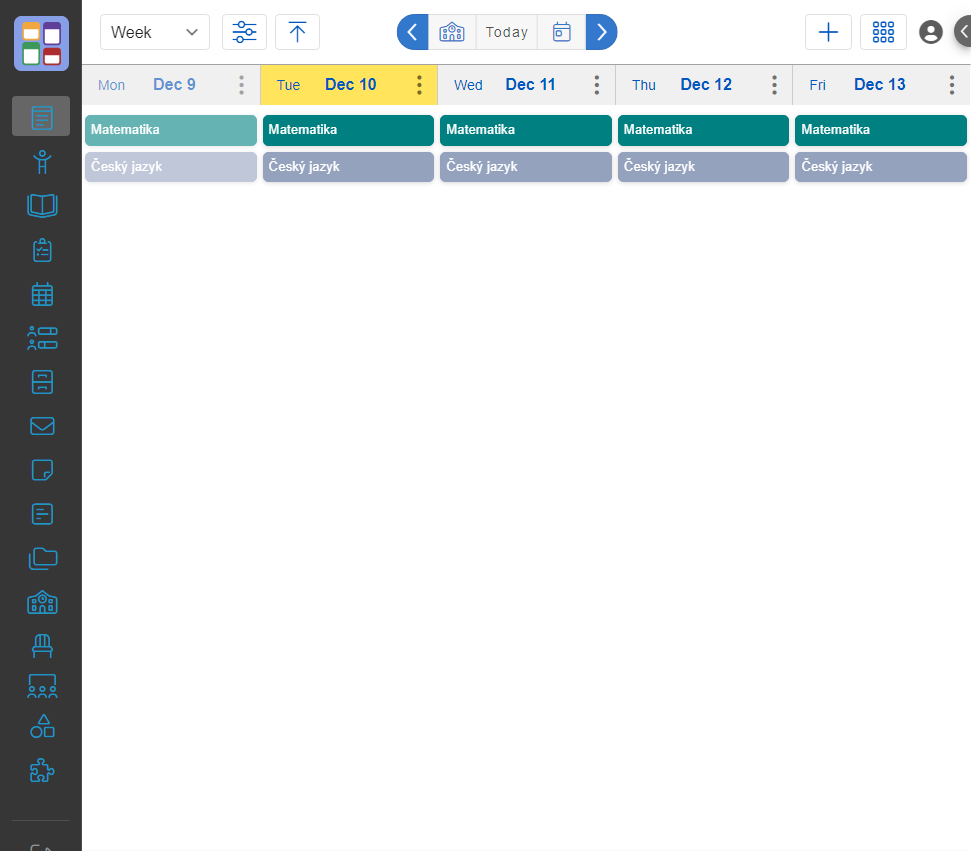
\includegraphics{planbook-1.png}}
	\caption{Okno aplikace Planbook s~náhledem na~kalendář.}
	\label{fig:planbook-1}
\end{figure}

\begin{figure}[H]
	\centering
	\resizebox{12cm}{!}{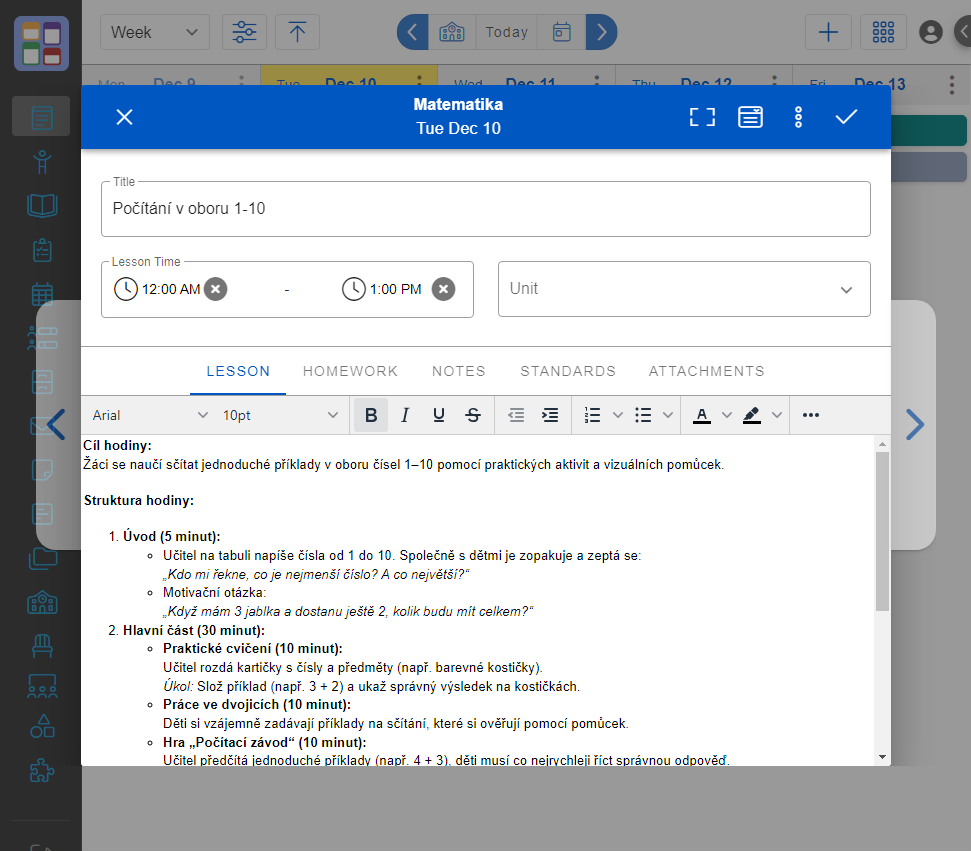
\includegraphics{planbook-2.png}}
	\caption{Okno aplikace Planbook s~náhledem na~editor výukového plánu.}
	\label{fig:planbook-2}
\end{figure}

\needspace{5\baselineskip}
\textbf{Hlavní funkce Planbook:}
\begin{itemize}
	\item více předmětů~--~učitelé mohou spravovat plány výuky pro~různorodé předměty,
	\item sdílení hodin~--~plány mohou být sdíleny se~studenty prostřednictvím jejich účtů,
	\item docházka a~známky~--~aplikace umožňuje evidenci docházky a~známek, což přidává další vrstvu organizace,
	\item WYSIWYG (What~You~See~Is~What~You~Get, intuitivní způsob editace textu) editor~--~pro tvorbu výukových hodin nabízí jednoduchý editor s~možností přidávání souborů a~poznámek.
\end{itemize}

\textit{Planbook} nabízí 90denní zkušební dobu. Následně stojí roční předplatné pro jednotlivce 20~dolarů, zatímco školní licence se pohybují mezi 14~až~18~dolary za~uživatele.

\subsection{Porovnání s~EDUBO}  
\textit{Planbook} i~\textit{EDUBO} se zaměřují na~digitální plánování výuky, ale jejich přístupy a~funkce se liší. Na~rozdíl od~\textit{Planbooku} nabízí \textit{EDUBO} lokalizaci do~češtiny a~robustnější editor plánů hodin, který umožňuje detailní strukturování výuky. Zatímco \textit{Planbook} obsahuje pokročilé funkce, jako je docházka a~známky, \textit{EDUBO} tyto funkce neřeší, protože se soustředí na~samotné plánování a~organizaci výuky. Významný rozdíl je také v~přístupu k~ceně~--~\textit{EDUBO} je zcela zdarma, zatímco \textit{Planbook} vyžaduje předplatné. Pokud jde o~spolupráci mezi učiteli, \textit{Planbook} ji nabízí v~placené verzi, kde učitelé mohou sdílet své plány. \textit{EDUBO} však tuto možnost rozšiřuje přes webový agregátor \textit{Eduklub~--~plány~výuky}, který je plně zdarma a~podporuje otevřenou spolupráci napříč uživateli.

\section{Common Curriculum}

\textit{Common~Curriculum} je další aplikace zaměřená na~plánování výuky, která je populární zejména mezi učiteli ve~Spojených~státech~amerických. Její hlavní předností je integrace amerických vzdělávacích standardů, což umožňuje snadné plánování výuky v~souladu s~těmito osnovami. Uživatelé mohou vytvářet plány pro různé předměty a~sdílet je buď prostřednictvím odkazu nebo v~PDF~formátu. Aplikace také umožňuje vytvořit třídní stránku, kde jsou zobrazeny rozvrhy spolu s~přehledy výukových plánů.

\begin{figure}[H]
	\centering
	\resizebox{12cm}{!}{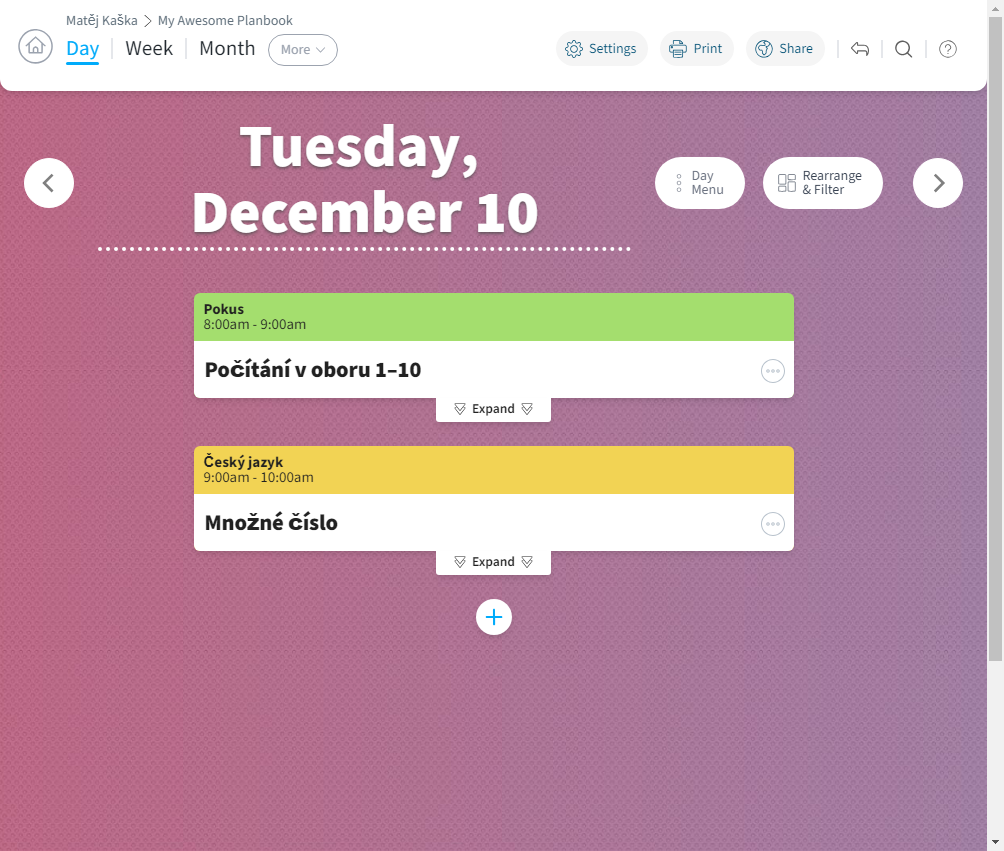
\includegraphics{common-curriculum-1.png}}
	\caption{Okno aplikace Common Curriculum s~náhledem na~kalendář.}
	\label{fig:common-curriculum-1}
\end{figure}
\begin{figure}[H]
	\centering
	\resizebox{12cm}{!}{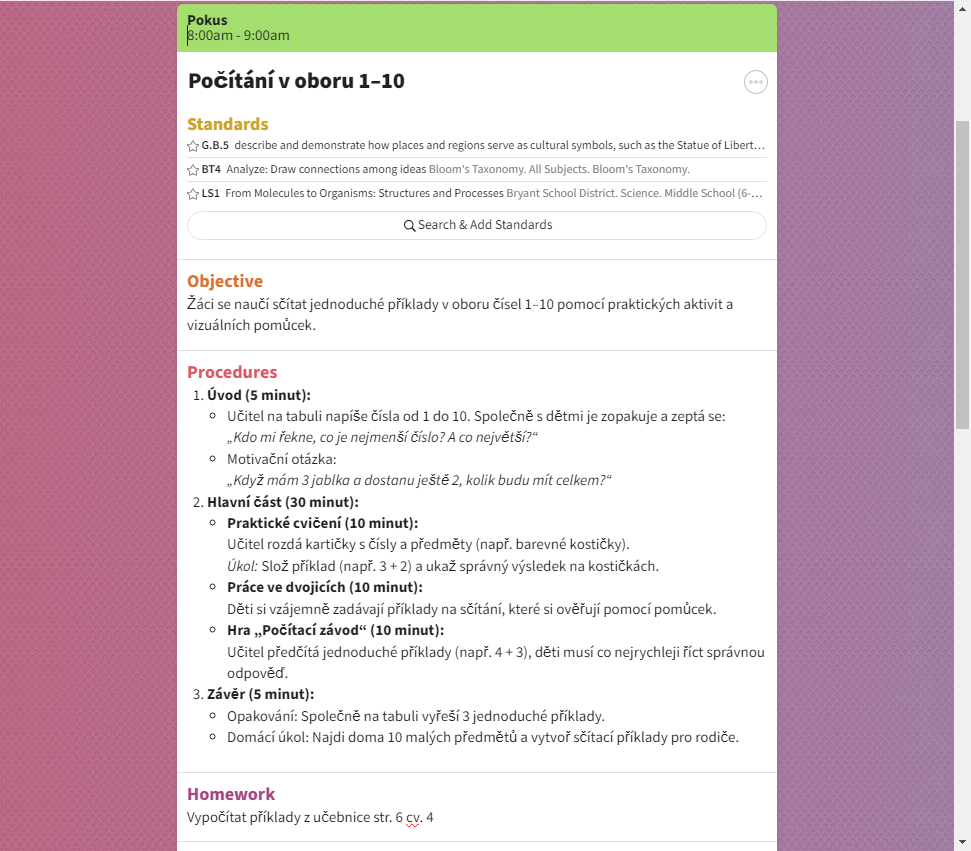
\includegraphics{common-curriculum-2.png}}
	\caption{Okno aplikace Common Curriculum s~náhledem na~editor výukového plánu.}
	\label{fig:common-curriculum-2}
\end{figure}

\needspace{6\baselineskip}
\textbf{Hlavní funkce Common Curriculum:}
\begin{itemize}
	\item více předmětů~--~učitelé mohou spravovat plány pro~předměty a~organizovat je podle tříd,
	\item integrace amerických vzdělávacích standardů~--~uživatelé mohou využívat předpřipravené kurikulární plány,
	\item možnosti sdílení~--~plány lze sdílet pomocí odkazu nebo exportovat do~PDF formátu,
	\item třídní stránka~--~učitelé mohou vytvořit přehled rozvrhů pro žáky a~rodiče,
	\item WYSIWYG editor~--~jednoduchý editor s~možností přidávat přílohy.
\end{itemize}

Aplikace nabízí bezplatnou verzi s~omezenými funkcemi, zatímco plná verze je dostupná za~8~dolarů měsíčně. Školní licence se odvíjejí od~počtu učitelů.

\subsection{Porovnání s~EDUBO}  
\textit{Common~Curriculum} a~\textit{EDUBO} sdílejí podobnou vizi v~oblasti plánování výuky, ale jejich funkcionalita a~přístup k~uživatelům se značně liší. \textit{Common~Curriculum} klade důraz na~americký vzdělávací systém, což je pro české prostředí nerelevantní. \textit{EDUBO} se naopak zaměřuje na~flexibilní tvorbu plánů přizpůsobených českému školství. Také editor je výrazně odlišný~--~zatímco \textit{Common~Curriculum} nabízí pouze textový editor, \textit{EDUBO} umožňuje rozdělit hodinu do~aktivit, přidávat cíle a~poznámky. V~oblasti spolupráce je \textit{EDUBO} výhodnější díky bezplatnému agregátoru plánů. Výhodu má \textit{EDUBO} rovněž v~ceně, jelikož je zcela zdarma.

\section{Lesson Planner PH}

\textit{Lesson~Planner~PH} je jednoduchá aplikace, která využívá umělou inteligenci k~automatickému generování plánů výuky a~testů. Podporuje pouze angličtinu a~filipínštinu a~nenabízí žádné další funkcionality kromě základního generování obsahu. Uživatelé mají měsíčně k~dispozici 30~bezplatných generování, přičemž další lze dokoupit prostřednictvím kreditového systému (1~generace za~přibližně~2~Kč).

Tato aplikace reflektuje současný trend využití umělé inteligence, který přináší jednoduchá řešení pro~tvorbu výukových materiálů. Nicméně, vzhledem k~absenci dalších funkcí, jako je strukturované plánování nebo správa tříd, není \textit{Lesson~Planner~PH} příliš vhodný pro~učitele, kteří potřebují propracovanější nástroj. \textit{EDUBO} naopak poskytuje širší škálu možností včetně propracovaného editoru a~lokalizace, což \textit{Lesson~Planner~PH} zcela postrádá. Na~druhou stranu však \textit{EDUBO} zatím postrádá integraci generativní umělé inteligence, která je jedním z~hlavních trendů současných vzdělávacích aplikací. Ačkoliv bylo v~plánu obohatit \textit{EDUBO} o~tyto funkce pro~automatické generování výukových plánů a~materiálů, tento rozvojový krok nebyl realizován kvůli nedostatečné podpoře projektu \textit{EDUZA}, jenž měl být zaměřen právě na tento typ funkcionality.

\section{Slides Go AI Lesson Plan Generator}

\textit{Slides~Go~AI~Lesson~Plan~Generator} je nástroj zaměřený na~rychlé generování plánů výuky pomocí umělé inteligence. Generované plány lze stáhnout v~PDF~formátu, ale aplikace nepodporuje český jazyk. \textit{Slides~Go} je zdarma a~svou jednoduchostí cílí na~učitele hledající rychlá a~snadná řešení.

Podobně jako \textit{Lesson~Planner~PH} odráží tento nástroj rostoucí trend využívání~AI v~oblasti vzdělávání, ale kvůli omezené funkčnosti nenabízí žádnou skutečnou přidanou hodnotu pro~komplexní plánování výuky. \textit{EDUBO} vyniká v~této oblasti tím, že umožňuje učitelům nejen detailní plánování, ale také jejich přizpůsobení a~sdílení s~kolegy a~studenty, což \textit{Slides~Go} zcela postrádá.

Tyto dvě aplikace ukazují, že současný trend umělé inteligence přináší řadu jednoduchých nástrojů pro~tvorbu výukových materiálů. Nicméně jejich omezená funkčnost a~absence pokročilých funkcí je činí spíše doplňkem než plnohodnotným řešením pro~plánování výuky, jakým je \textit{EDUBO}.

\chapter{Teoretická východiska}
\section{Výukový proces}

Porozumění výukovému procesu je pro~každého vyučujícího klíčové, protože právě skrze něj se uskutečňuje efektivní přenos znalostí a~dovedností. Výukový proces není pouze o~předávání informací, ale o~vědomém a~promyšleném řízení výuky tak, aby došlo k~porozumění, zapamatování a~aplikaci učiva. Pro~vyučujícího to znamená nejen znalost látky, ale i~schopnost zvolit vhodné metody, nástroje a~strategie, které podpoří proces učení u~každého jednotlivého žáka.

Jedním z~často citovaných modelů, který pomáhá pochopit strukturu efektivního vyučování,\break je Gagného devíti krokový model (\textit{Nine~Events~of~Instruction}). Americký psycholog\break\mbox{Robert~Mills~Gagné,~A.B.,~Sc.M.,~Ph.D.}, vytvořil tuto strukturu jako vodítko pro~učitele k~postupnému vedení výuky. Jeho devět kroků lze shrnout následovně:

\begin{enumerate}
	\item \textbf{Získání pozornosti} (\textit{Gaining attention})~--~Například pomocí otázky, překvapivého faktu nebo vizuálního stimulu.
	\item \textbf{Informování o~cílech výuky} (\textit{Informing learners of objectives})~--~Učící se by měl vědět, co~se má naučit.
	\item \textbf{Navázání na~předchozí znalosti} (\textit{Stimulating recall of prior learning})~--~Aktivace dřívějších znalostí a~zkušeností.
	\item \textbf{Prezentace obsahu} (\textit{Presenting the stimulus})~--~Podání nové látky vhodnou formou.
	\item \textbf{Poskytnutí vedení} (\textit{Providing "learning guidance"})~--~Poskytnutí vodítek, která pomáhají učícímu se propojit nové informace do~smysluplného celku.
	\item \textbf{Vybídnutí k~praxi} (\textit{Eliciting performance})~--~Možnost procvičení nebo vyzkoušení nového učiva.
	\item \textbf{Poskytnutí zpětné vazby} (\textit{Providing feedback})~--~Okamžitá zpětná vazba učícímu se.
	\item \textbf{Zhodnocení výstupu} (\textit{Assessing performance})~--~Ověření, zda se učící se učivo naučil, například formou testu, diskuse nebo praktického úkolu.
	\item \textbf{Podpora zapamatování a~přenosu nově osvojených znalostí} (\textit{Enhancing retention and transfer})~--~Pomoc učícím se, aby si nové poznatky zapamatovali a~uměli je aplikovat v~praxi.
\end{enumerate}
\noindent
\textit{Volně přeloženo z~\cite[s.~246]{gagne1985conditions}.}

Tento model je cenný zejména svou přehledností a~univerzálností~--~lze jej aplikovat jak při přípravě běžné vyučovací hodiny, tak při tvorbě digitálních výukových materiálů. 

Pohled na~výukový proces rozšířil také Pavel~Beránek, který jej ve~své přednášce popsal jako interakci dvou subjektů~--~vyučujícího a~učícího se. Výuková látka je vyučujícím nejprve didakticky transformována, tedy přetvořena do~podoby, která je vhodná pro~předání a~následně předávána učícímu se. Ten ji zpracovává (asimiluje) svým vlastním tempem a~způsobem. Cílem práce vyučujícího je optimalizovat celý tento proces tak, aby bylo učení co~nejefektivnější.

Výuka však vždy probíhá v~určité formě, která ji výrazně ovlivňuje. Tato forma zahrnuje například místo výuky, časové zařazení (dopoledne nebo odpoledne) a~také způsob výkladu, tedy zda vyučující látku pouze přednáší, vede diskusi nebo nechává učící se pracovat samostatně. Výběr těchto parametrů má zásadní vliv na~výkon učících se~--~například náročné učivo zařazené na~konec dne celodenní výuky může být méně efektivní než stejné učivo vyučované na~začátku dne.

Výukový proces je zároveň ovlivněn mnoha determinanty, které lze rozdělit na~interní a~externí. Interní determinanty zahrnují například mentální schopnosti učících se, úroveň porozumění, motivaci či případné specifické poruchy učení. Tyto faktory mohou být částečně ovlivnitelné, avšak mnohdy je nutné je zohlednit při výběru přístupů a~metod. Mezi externí determinanty spadá prostředí třídy, hladina hluku, světelné podmínky, čas výuky nebo dostupné pomůcky.

Podstatným prvkem efektivní výuky je také volba vhodných nástrojů a~pomůcek. Ty mohou být jak tradiční (tabule, učebnice, abakus), tak moderní (interaktivní tabule, výukové aplikace, experimentální sady). Správně zvolené pomůcky usnadňují pochopení látky a~mohou posílit motivaci učících se.

Didaktické strukturování hodiny do~výukových aktivit umožňuje lépe řídit průběh výuky a~přizpůsobit ji rytmu pozornosti učících se. Délka jednotlivých aktivit, jejich náplň a~návaznost mají vliv na~to, jak učící se vnímají a~zpracovávají učivo. Dobře připravený plán s~různorodými aktivitami zvyšuje efektivitu výuky a~umožňuje vyučujícímu pružně reagovat na~potřeby třídy.

Závěrem je nutné zmínit také testování asimilace, tedy ověření toho, zda se učící se skutečně naučili to, co~bylo cílem výuky. Rozlišujeme sumativní testování, které poskytuje celkový přehled o~dosažených výsledcích (např.~test na~konci kapitoly) a~formativní hodnocení, které probíhá průběžně a~slouží jako zpětná vazba pro~vyučujícího i~učícího se. Může mít podobu diskuse, otázek během výuky nebo jednoduchého dotazu při individuálním kontaktu.

\begin{figure}[H]
	\centering
	\resizebox{15.125cm}{!}{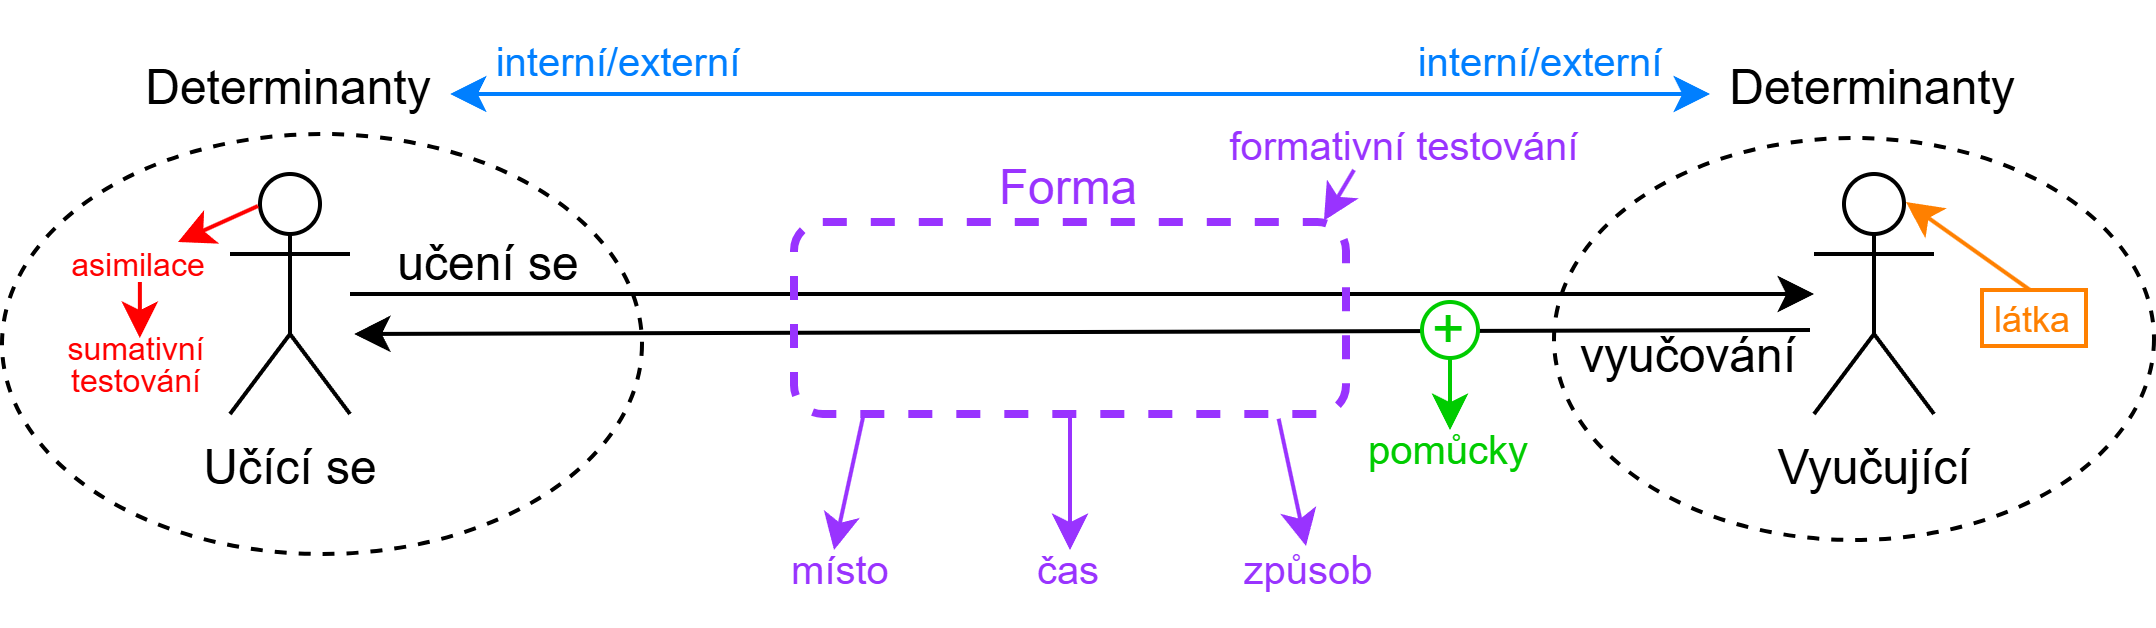
\includegraphics{vyukovy-proces.png}}
	\caption{Převzatý diagram z \cite{beranek2025} znázorňující výukový proces navržený Pavlem Beránkem.}
	\label{fig:vyukovy-proces}
\end{figure}

\section{Výukové aktivity}
Výukové aktivity tvoří základní nástroje, pomocí kterých učitel strukturuje a~řídí proces učení. Nejde pouze o~plnění úkolů, ale o~promyšlené činnosti, které naplňují konkrétní výukové cíle, zapojují žáky a~pomáhají budovat hlubší porozumění. Jejich správný výběr a~zařazení do~hodinové struktury přispívá k~efektivnějšímu učení. Mezi klíčové typy aktivit patří např.~evokace, objevování, procvičování, výklad, shrnutí, hodnocení, práce se~zdroji či zpětná vazba.

\subsection{Evokace}

Evokace představuje úvodní fázi výukové hodiny a~její hlavní funkcí je připravit žáky na~výuku. Správně zvládnutý začátek hodiny je předpokladem pro~úspěšné učení. Učitel v~této fázi pracuje s~pozorností, motivací, cíli a~navázáním na~předchozí znalosti žáků. Účelem je zajistit, aby žáci věděli, co~se budou učit, proč je to důležité, a~zároveň se cítili připraveni na~nové učivo.\cite{eduEvokace}

\subsubsection{Aktivace předchozích znalostí}
Jednou z~klíčových aktivit v~rámci evokace je aktivace vstupních znalostí, kdy učitel zjišťuje, co~žáci o~tématu už vědí. Může využít brainstorming (burza nápadů), otázky, digitální nástroje (např.~Mentimeter) nebo krátké úlohy. Výsledky se doporučuje vizualizovat, aby s~nimi bylo možné dále pracovat.\cite{eduAktivovaniVstupnichZnalosti}

\subsubsection{Stanovení cílů}
Další důležitou aktivitou v~úvodu hodiny je sdělení výukového cíle. Dobře formulovaný cíl by měl být konkrétní, ověřitelný a~formulovaný z~pohledu žáka~--~např.~\quotedblbase žák na~konci hodiny rozliší\ldots``. Formulace cílů může vycházet z~Bloomovy taxonomie nebo její revidované verze, která rozlišuje dimenzi znalostí a~kognitivních procesů. Stanovení cíle dává výuce směr a~umožňuje učiteli i~žákovi reflektovat pokrok.\cite{eduStanoveniCilu}

\subsection{Hodnocení}
Hodnocení je jednou ze~součástí vzdělávacího procesu. Jeho cílem je poskytnout žákům zpětnou vazbu a~podporu pro~jejich další učení a~rozvoj. Mělo by být konstruktivní, pozitivní a~objektivní. Hodnocení neslouží jen ke~klasifikaci, ale i~k~identifikaci oblastí, na~kterých je třeba dále pracovat. Důležité je vytvořit podpůrné a~bezpečné prostředí, kde stres z~výsledků není překážkou v~učení. Hodnocení tak může být nástrojem rozvoje, ne trestu.\cite{eduHodnoceni}

\newpage

\subsubsection{Kontrolní test}
Kontrolní test může mít písemnou nebo praktickou podobu. Slouží k~ověření znalostí a~dovedností v~rámci aktuálně probírané oblasti. V~praktické podobě může žák například něco vytvořit, opravit či navrhnout. Testy mohou zahrnovat různé typy otázek~--~otevřené, uzavřené, shody nebo doplňování vět.\cite{eduKontrolniTest}

\subsubsection{Souhrnný test}
Souhrnný test ověřuje zvládnutí učiva za~delší časové období, např.~na~konci tematického celku, čtvrtletí nebo pololetí. Mívá širší záběr než běžné testy a~může mít písemnou nebo praktickou formu. Záměrem není jen ověřit paměťové zvládnutí faktů, ale také schopnost propojit klíčové koncepty a~dovednosti.\cite{eduSouhrnnyTest}

\subsubsection{Ústní zkoušení}
Ústní zkoušení může být pro~některé žáky stresující. Je důležité žáky na~jeho průběh připravit, poskytnout jim jasné informace o~jeho cíli a~průběhu. Důraz by měl být kladen na~porozumění, nikoli na~formu. Alternativou může být projekt, prezentace nebo týmová práce.\cite{eduUstniZkouseni}

\subsubsection{On-line testování}
On-line testování poskytuje okamžitou zpětnou vazbu, umožňuje personalizaci testu a~efektivní sledování pokroku žáků. Díky automatickému hodnocení je časově efektivní a~umožňuje rychlé vyhodnocení odpovědí. Test může být proveden na~různých zařízeních~--~mobilních telefonech, tabletech i~počítačích.\cite{eduOnlineTestovani}

\subsubsection{Skupinové testování}
Skupinové testování je forma hodnocení, která rozvíjí nejen znalosti a~dovednosti, ale také schopnost komunikace a~spolupráce. Test není soutěž, ale příležitost pro~vzájemné učení. Žáci by měli být předem seznámeni s~hodnoticími kritérii. Správně vedené skupinové testování pomáhá posilovat sociální dovednosti i~kritické myšlení.\cite{eduSkupinoveTestovani}

\subsection{Objevování}

Objevování neboli \quotedblbase umění objevovat`` označuje metodologický přístup k~poznání založený na~uvědomění si existence určitých pravidelností, které dosud nebyly ověřeny. Žáci nejsou pasivními příjemci informací, ale sami přicházejí na~nové poznatky prostřednictvím vlastního bádání, srovnávání, kladení otázek a~vytváření hypotéz. Didaktickým cílem objevování je zapojit žáky do~procesu samostatného řešení problémů a~podpořit jejich tvůrčí myšlení.

Objevování může mít podobu heuristického rozhovoru nebo výkladu, přičemž žáci pracují s~otázkami, modely, schématy či analogiemi. Výuka založená na~heuristických funkcích stimuluje žáky k~aktivnímu učení, hlubšímu porozumění a~integraci znalostí. Učitel může zvolit \quotedblbase malou`` nebo \quotedblbase velkou`` heuristickou metodu~--~podle míry samostatnosti žáka při zpracování učiva.\cite{eduObjevovani}

\subsubsection{Práce se~zdroji, příklady a~situacemi}

Žáci se učí využívat dostupné informační zdroje, pracují s~texty, obrázky, animacemi nebo simulačními programy. Výuka může být zaměřena na~vyhledávání informací, jejich prezentaci, práci s~výukovým softwarem nebo tvorbu vlastních výstupů. Učitel by měl nabídnout vhodné okruhy nebo odkazy a~důsledně promyslet činnosti žáků po~stránce metodické i~obsahové.\cite{eduPraceSeZdrojiPrikladySituacemi}

\subsubsection{Pracovní listy}

Pracovní listy vedou žáky k~aktivnímu zkoumání a~kritickému myšlení. Mohou obsahovat otázky, úkoly nebo úlohy k~analýze konkrétního problému. Pracovní listy lze využít při individuální, párové i~skupinové práci.\cite{eduPracovniListy}

\subsubsection{Bádání}

Badatelsky orientované učení podporuje koncepční porozumění a~proces osvojování znalostí skrze vlastní aktivitu žáka. Žáci formulují problémy, navrhují způsoby řešení, analyzují a~ověřují data. Podle míry vedení učitelem lze rozlišit čtyři úrovně bádání~--~potvrzující, strukturované, nasměrované a~otevřené.\cite{eduBadani}

\subsubsection{Experiment}

Experiment slouží k~ověřování hypotéz a~poznání za~řízených podmínek. Může mít formu kvalitativní, kvantitativní nebo myšlenkovou. Během experimentu žáci pozorují, měří, analyzují data a~vyvozují závěry. Významnou roli hraje i~plánování a~zpracování výsledků.\cite{eduExperiment}

\subsubsection{On-line experiment}

On-line experimenty zpřístupňují vzdálená měření nebo přístroje, které by jinak byly žákům nedostupné. Žáci mohou získávat data z~reálných měření například prostřednictvím meteorologických stanic nebo vzdálených laboratoří.\cite{eduOnlineExperiment}

\newpage

\subsubsection{Simulace}

Simulace představují využití virtuálního prostředí k~modelování jevů, které jsou nebezpečné, obtížně přístupné nebo abstraktní. Ve~výuce se využívají například simulace měření, modelování molekul nebo virtuální laboratoře. Tyto nástroje pomáhají vizualizovat procesy a~zprostředkovat poznání jinou formou než tradiční experiment.\cite{eduSimulace}

\subsection{Zdroje}

Práce se~zdroji představuje důležitou výukovou aktivitu, která rozvíjí kritické myšlení, informační gramotnost a~schopnost samostatného učení. Žáci se neučí pouze pasivně přijímat předložené informace, ale také sami vyhledávat relevantní a~důvěryhodné zdroje, posuzovat jejich kvalitu a~ověřovat fakta. Učitelé je přitom vedou k~rozpoznání spolehlivosti informací, zohlednění různých pohledů na~téma a~etickému zacházení s~informacemi. Klíčem je podpora samostatnosti a~schopnosti žáků aktivně se~zapojit do~vzdělávacího procesu prostřednictvím informací z~různých typů zdrojů.\cite{eduPraceSeZdroji}

\subsubsection{Sběr dat}

Sběr dat je aktivitou, při které žáci sami získávají informace prostřednictvím vlastních měření, dotazníků nebo pozorování. Tento způsob práce vede k~praktické zkušenosti, rozvoji kritického myšlení i~zapojení do~místně zakotveného učení. Žáci se učí třídit a~interpretovat data, která mají pro~ně osobní význam, a~zároveň mohou rozvíjet i~komunikační dovednosti.\cite{eduSberDat}

\subsubsection{On-line zdroje}

On-line prostředí nabízí široké spektrum informačních materiálů~--~od~odborných databází po~běžně navštěvované portály. Práce s~těmito zdroji rozvíjí nejen digitální kompetence, ale především schopnost hodnotit důvěryhodnost, relevanci a~účel obsahu. Učitelé vedou žáky k~tomu, aby při vyhledávání informací zvažovali nejen co, ale i~proč a~od~koho čerpají.\cite{eduOnlineZdroje}

\subsubsection{Práce s~literaturou}

Tištěné materiály, jako slovníky, tabulky, grafy nebo mapy, umožňují žákům porozumět obsahu do~hloubky a~trénovat dovednosti spojené s~vyhledáváním a~interpretací dat. Práce s~knihou podporuje i~dovednosti potřebné pro~akademickou přípravu.\cite{eduPraceSLiteraturou}

\newpage

\subsubsection{Počítačové simulace ve~výuce}

Simulace umožňují žákům interaktivní a~bezpečné zkoumání složitých jevů~--~například vizualizací pohybu, chemických reakcí nebo sociálních interakcí. Zajišťují okamžitou zpětnou vazbu a~podporují aktivní učení, analýzu výsledků a~kreativitu. Jejich dostupnost a~rozmanitost umožňuje efektivní využití napříč obory a~stupni vzdělávání.\cite{eduPocitacoveSimulace}

\subsection{Procvičování}

Procvičování je základním stavebním kamenem efektivního vzdělávání. Umožňuje žákům upevnit znalosti, přenést je do~dlouhodobé paměti a~osvojit si automatizované dovednosti. Klíčem je pravidelnost, rozmanitost a~cílené opakování. Kombinace různých typů úloh, praktické aplikace a~poskytnutí zpětné vazby podporují hlubší porozumění a~motivují k~dalšímu učení. Významnou roli zde sehrává i~technologie, která umožňuje individualizaci výuky a~okamžitou odezvu na~výkon žáků.\cite{eduProcvicovani}

\subsubsection{Receptivní a~produktivní jazykové dovednosti}

Procvičování zahrnuje aktivity zaměřené na~všechny složky jazykového projevu. Čtení a~poslech rozvíjejí schopnost porozumět tištěným i~audiovizuálním materiálům. Mluvení a~psaní vedou k~aktivní produkci, kde žáci uplatňují získané poznatky ve~vlastním projevu. Všechny tyto dovednosti se uplatňují v~komunikaci, často i~formou interakce mezi spolužáky, která přirozeně propojuje jazyk s~reálnými situacemi.\cite{eduCteni}\cite{eduPsani}\cite{eduPoslech}\cite{eduMluveni}\cite{eduInterakce}

\subsubsection{Procvičování s~využitím ICT}

Digitální nástroje jako Google~Forms, Kahoot! nebo Quizlet umožňují rychlé a~variabilní procvičování s~okamžitou zpětnou vazbou. Podporují motivaci žáků, ulehčují sledování pokroku a~umožňují efektivní diferenciaci výuky.\cite{eduProcvICT}

\subsubsection{Mediace}

Mediace představuje schopnost zprostředkovat informaci dalším osobám~--~shrnout, přeložit, vysvětlit či přetvořit původní sdělení tak, aby bylo srozumitelné. Umožňuje žákům propojit porozumění a~produkci, rozvíjí samostatnost a~schopnost přizpůsobit jazyk různým situacím a~adresátům.\cite{eduMediace}

\subsubsection{Manipulativní činnosti}

Práce s~konkrétními objekty pomáhá rozvíjet jemnou motoriku, prostorové vnímání, ale i~schopnost spolupráce a~řešení problémů. Rýsování, stavění modelů nebo praktická měření přinášejí aktivní zapojení žáků a~podporují jejich učení prostřednictvím více smyslů.\cite{eduManipulativniCinnosti}

\subsubsection{Herní aktivity}

Hra vytváří přirozené a~motivující prostředí pro~učení. Využívá soutěživost, ale i~spolupráci. Jazyk a~poznatky jsou aplikovány nenásilně, což napomáhá jejich osvojení. Didaktické hry umožňují procvičování i~evaluaci bez~stresu z~formálního hodnocení.\cite{eduHra}

\subsection{Shrnutí}

Závěrečné shrnutí je důležitou součástí hodiny. Nejde jen o~zopakování, co~se v~hodině dělo, ale hlavně o~zdůraznění podstatného a~propojení na~další témata. Shrnutí pomáhá utvrdit učivo, dává žákům přehled, kontroluje porozumění a~podporuje aktivní učení. Má také pozitivní vliv na~motivaci a~přípravu na~domácí úkoly nebo zkoušení.\cite{eduShrnuti}

\subsubsection{Had}

Had je jednoduchá, ale efektivní metoda shrnutí učiva, při které každý žák stručně sdělí, co~si z~hodiny odnáší. Postupuje se po~třídě, jeden po~druhém~--~vzniká tak pomyslný \quotedblbase had``. Vyučující může žáky omezit na~jedno či dvě slova, případně zadání ztížit tím, že každý musí říct něco, co~ještě nezaznělo. Aktivita posiluje soustředění, sebereflexi a~dává učiteli rychlou zpětnou vazbu o~tom, co~žáci vnímají jako důležité.\cite{eduHad}

\subsubsection{Propustky}

Propustky jsou shrnovací technika, při které žáci na~konci hodiny vyplní malý lístek s~odpovědí na~zadanou otázku~--~např.~\quotedblbase Co~si z~hodiny odnášíš?“, případně \quotedblbase Čemu jsi nerozuměl?“. Mohou být anonymní, což podporuje upřímnost a~pocit bezpečí. Učitel získává rychlý přehled o~pochopení učiva i~tématech, ke~kterým je potřeba se vrátit. Propustky jsou nenáročné na~přípravu a~dají se snadno začlenit do~jakékoliv výuky.\cite{eduPropustky}

\subsubsection{Myšlenkové mapy}

Myšlenkové mapy slouží jako vizuální nástroj pro~shrnutí učiva, který pomáhá zapamatování, třídění informací a~rozvíjí kreativitu. Lze je využít při prezentacích, brainstormingu, plánování, řešení problémů i~alternativních zápiscích.\cite{eduMyslenkoveMapy}

\subsubsection{Otázky}

Otázky jsou klíčovým nástrojem zpětné vazby. Pomáhají učiteli zjistit míru porozumění a~žákům třídit myšlenky. Měly by být promyšlené, navázané na~výukové cíle a~přizpůsobené úrovni žáků. Kromě faktických dotazů je vhodné používat otázky vyšší kognitivní úrovně\break(např.~podle Bloomovy taxonomie), otevřené otázky nebo techniky jako \textit{Think~--~Pair~--~Share\break(Mysli~--~Diskutuj~ve~dvojici~--~Sdílej)}.\cite{eduOtazky}

\subsection{Výklad}

Výklad je metoda, při které učitel slovně předává nové informace a~vysvětluje význam učiva. Patří mezi nejběžnější formy výuky, umožňuje rychle a~efektivně seznámit žáky s~novým tématem. Aby byl výklad co~nejúčinnější, měl by být srozumitelný, strukturovaný, doplněný vizuální oporou a~proložený aktivizačními prvky.\cite{eduVyklad}

\subsubsection{Struktura učiva}

Seznámení žáků s~cíli a~strukturou učiva na~začátku tématu podporuje jejich motivaci, orientaci a~pochopení. Jasný rámec výuky pomáhá lépe plánovat další aktivity a~rozvíjí i~kritické myšlení žáků.\cite{eduStrukturaUciva}

\subsubsection{Vizualizace}

Teorie duálního kódování vysvětluje, proč si žáci lépe zapamatují informaci, pokud ji slyší a~zároveň vidí. Mozek totiž zpracovává informace pomocí dvou oddělených kanálů: verbálního (slova) a~vizuálního (obrazy). Když tyto kanály propojujeme, snižujeme zatížení pracovní paměti a~zvyšujeme šanci na~hlubší učení, zejména u~dětí starších sedmi let. Výzkumy ukazují, že např.~při učení slovíček pomáhá jejich propojení s~odpovídajícími obrázky. V~hodinách tak dává smysl kombinovat výklad s~vhodnými vizuálními prvky.\cite{eduVizualizace}

\subsubsection{Praktické příklady}

Použití konkrétních příkladů, modelů nebo běžných životních situací přibližuje učivo realitě a~podporuje hlubší porozumění. Žáci si lépe zapamatují to, co~si dokáží představit nebo si sami vyzkoušet.\cite{eduPraktickePriklady}

\subsubsection{Modely}

Modely chápeme jako názorné učební pomůcky, které pomáhají konkretizovat abstraktní pojmy a~objasnit vztahy nebo procesy. Měly by být názorné, věrné a~přiměřeně zjednodušené. Důležité je, aby žáci chápali rozdíl mezi modelem a~skutečností.\cite{eduModely}

\subsection{Zpětná vazba}

Zpětná vazba je klíčovou součástí formativního hodnocení. Než ji poskytneme, musíme mít jasné cíle a~kritéria hodnocení. Efektivní zpětná vazba popisuje, co~se žákovi podařilo, a~místo přímé kritiky klade otázky, které vedou k~zamyšlení. Správně podaná zpětná vazba by měla žáka motivovat a~vést ke~zlepšení výkonu, nikoliv ho demotivovat nebo hodnotit jako osobnost.\cite{eduZpetnaVazba}

\subsubsection{Signál}

Signál je jednoduchá technika pro~okamžité zjištění, zda žáci porozuměli učivu. Pomocí palců, symbolů nebo kartiček dávají žáci najevo, jestli učivo chápou, mají pochybnosti nebo nerozumí. Výhodou je rychlá vizuální zpětná vazba, kterou učitel získá od~celé třídy najednou. Tato metoda posiluje participaci a~učí žáky reflektovat své vlastní porozumění.\cite{eduSignal}

\subsubsection{Teploměr}

Teploměr slouží k~vizuálnímu vyjádření pocitu porozumění nebo nálady žáků na~škále. Umožňuje jim sledovat svůj pokrok nebo míru pochopení v~čase. Pomocí procent nebo symbolů si žáci sami označují, jak se cítí nebo jak rozumí probíranému tématu. Tato metoda podporuje sebereflexi a~umožňuje učiteli lépe přizpůsobit výuku.\cite{eduTeplomer}

\subsubsection{Škála}

Škála je nástroj, pomocí kterého mohou žáci vyjádřit, jak dobře se cítí ve~vztahu k~probírané látce nebo aktivitě. Často se využívá čtyř až desetistupňové hodnocení. Učitel získává subjektivní, ale užitečný pohled na~vnímání výuky ze~strany žáků. Škála se může týkat nejen porozumění, ale i~emocí a~spolupráce.\cite{eduSkala}

\subsubsection{Semafor}

Semafor je oblíbená technika, při níž žáci pomocí tří barev vyjadřují úroveň porozumění. Zelená značí úplné porozumění, oranžová nejistotu a~červená neporozumění. Učitel okamžitě získává přehled o~stavu třídy a~může reagovat. Žáci se zároveň učí hodnotit sami sebe a~nebát se přiznat problém.\cite{eduSemafor}

\subsubsection{Mazací tabulky}

Mazací tabulky žáci využívají k~zaznamenání krátkých odpovědí, výpočtů, náčrtků, grafů nebo jazykových jevů, které následně na~pokyn učitele ukazují. Tím poskytují rychlou zpětnou vazbu o~své úrovni porozumění, aniž by museli vystupovat veřejně. Tato technika rozvíjí schopnost přesné formulace myšlenek a~je snadno použitelná v~různých předmětech.\cite{eduMazaciTabulky}

\subsubsection{Losovátka a~špachtličky}

Losovátka přinášejí do~výuky prvek náhody a~spravedlnosti. Učitel si připraví např.~dřevěné špachtle, na~které napíše jména všech žáků, a~vloží je do~kelímku. Po~položení otázky učitel jednu ze~špachtlí náhodně vytáhne a~ta určí, kdo bude odpovídat. Tímto způsobem se udržuje pozornost celé třídy a~aktivizují se i~ti, kteří se běžně nehlásí. Tento způsob zajišťuje spravedlnost a~udržuje všechny ve~střehu.\cite{eduLosovatka}

\subsubsection{Think~--~Pair~--~Share}

\textit{Think~--~Pair~--~Share~(Mysli~--~Diskutuj~ve~dvojici~--~Sdílej)} dává žákům čas na~přemýšlení, diskuzi a~následné sdílení. Učitel nejprve položí otázku, pak žáci diskutují ve~dvojicích, a~nakonec jeden z~nich odpoví. Tato metoda podporuje hlubší zamyšlení a~spolupráci. Introverti mají šanci připravit si odpověď, extroverti se učí strukturovat své myšlenky.\cite{eduThinkPairShare}

\subsubsection{Barevné kelímky}

Barevné kelímky pomáhají žákům vizuálně vyjádřit, v~jaké fázi práce se právě nachází. Každý má na~lavici sadu kelímků různých barev~--~např.~bílý \quotedblbase pracuji``, zelený \quotedblbase mám hotovo a~mohu pomoci``, žlutý \quotedblbase potřebuji pomoc od~spolužáka`` a~červený \quotedblbase nerozumím a~potřebuji pomoc učitele``. Žák jednoduše postaví na~lavici kelímek dané barvy podle své situace. Učitel tak získává okamžitý přehled o~třídě a~může efektivně reagovat. Zároveň se tím podporuje vzájemná spolupráce a~vrstevnická výpomoc, která rozvíjí jak žáky, kteří pomoc poskytují, tak ty, kteří ji přijímají.\cite{eduBarevneKelimky}

\subsubsection{Nedokončené věty}

Nedokončené věty slouží žákům k~tomu, aby na~konci hodiny reflektovali svůj učební proces. Učitel jim nabídne začátek věty, jako např.~\quotedblbase Zlepšil jsem se v\ldots`` nebo \quotedblbase Nejvíce mě zaujalo\ldots``, a~žáci ji dokončí podle svých zkušeností z~hodiny. Tato technika rozvíjí schopnost sebereflexe, podporuje vědomé učení a~pomáhá žákům lépe formulovat, co~potřebují ke~zlepšení. Výhodou je, že se aktivně zapojují i~ti, kteří se v~hodině běžně tolik neprojevují.\cite{eduNedokonceneVety}

\subsubsection{Otevřené otázky}

Otevřené otázky rozvíjejí kritické myšlení a~samostatné vyjadřování žáků. Učitel se skrze ně dozvídá více než jen fakta~--~například i~o~emocích nebo způsobu práce žáka. Je třeba klást jasně formulované otázky bez~náznaku správné odpovědi. Tato technika je vhodná pro~hlubší porozumění a~plánování další výuky.\cite{eduOtevreneOtazky}

\subsubsection{Učební úloha}

Učební úloha slouží k~tomu, aby se žák něco naučil~--~na~rozdíl od~testové, která jen ověřuje. Žáci mohou pracovat samostatně, ve~dvojicích nebo se~zdroji, pokud se úloha zaměřuje na~vyšší kognitivní náročnost. Učební úlohy často fungují jako diagnostický nástroj na~konci hodiny.\cite{eduUcebniUloha}

\subsubsection{Komplexní způsob hodnocení}

Komplexní hodnocení propojuje formativní a~sumativní přístupy a~vedle známek zahrnuje i~slovní zpětnou vazbu, reflexi a~povzbuzení. Klade důraz na~proces učení, nikoliv jen na~jeho výsledek. Učitel spolu se~žákem sleduje, kde se žák nachází, a~společně hledají cesty ke~zlepšení. Žáci se učí hodnotit nejen práci druhých, ale i~sami sebe, což rozvíjí jejich metakognitivní dovednosti a~zvyšuje zodpovědnost za~vlastní učení. Smyslem tohoto přístupu je nejen zlepšit výsledky, ale vést žáky k~hlubšímu porozumění a~dlouhodobému růstu.\cite{eduKomplexniZpusobHodnoceni}


\section{Životní cyklus softwaru}

Životní cyklus softwaru představuje chronologicky propojenou soustavu stavů, kterými software postupně prochází od~počátečního návrhu až po~finální údržbu. Tento cyklus zahrnuje všechny kroky nutné k~vytvoření kvalitního produktu, který odpovídá potřebám uživatelů a~zadavatelů. Životní cyklus je přizpůsobitelný různým typům projektů a~metodikám, což z~něj činí univerzální rámec vhodný pro~malé i~rozsáhlé projekty. Jeho správné řízení zajišťuje efektivitu vývoje a~umožňuje reagovat na~změny v~průběhu celého projektu. Životní cyklus softwaru je řízen procesem vývoje softwaru.

Proces vývoje softwaru je systematický a~strukturovaný přístup, jehož cílem je vytvořit spolehlivý a~funkční produkt. Tento proces minimalizuje rizika a~chyby, optimalizuje využití zdrojů a~zajišťuje splnění jak funkčních, tak mimofunkčních požadavků. Každá fáze vývoje, od~analýzy a~návrhu přes implementaci až po~testování a~nasazení, má jasně stanovené cíle a~výstupy, které tvoří základ pro~další kroky. Strukturovaný proces navíc podporuje týmovou spolupráci a~usnadňuje komunikaci mezi členy týmu, vedením projektu a~uživateli, čímž přispívá k~hladkému průběhu vývoje.

\subsection{Fáze životního cyklu softwaru}

Životní cyklus softwaru se skládá z~několika základních fází, z~nichž každá plní specifickou funkci a~přispívá k~dosažení cílového produktu. Jednotlivé fáze na~sebe logicky navazují, přičemž jejich průběh může být lineární (např.~vodopádový model) nebo iterativní (např.~agilní přístupy).\cite{softwaroveInzenyrstviSem1}

\subsubsection{Analýza}

Fáze analýzy je klíčovým počátečním krokem životního cyklu. Během této fáze se sbírají a~analyzují požadavky uživatelů a~stakeholderů (zainteresovaných stran). Hlavním cílem analýzy je pochopit, jaké funkce a~vlastnosti má výsledný software mít, a~vytvořit tak pevný základ pro~následný návrh a~vývoj.

\needspace{4\baselineskip}
V~této fázi dochází k~definování:
\begin{itemize}
	\item funkčních požadavků (co má software dělat, např.~možnost registrace uživatele),
	\item mimofunkčních požadavků (např.~výkon, bezpečnost, škálovatelnost),
	\item základních cílů projektu (např.~časový harmonogram, rozpočet, klíčové milníky).
\end{itemize}

\needspace{5\baselineskip}
V~rámci analýzy požadavků se požadavky často rozdělují do~tří kategorií:
\begin{itemize}
	\item \textbf{normální požadavky (normal)}~--~standardní funkce, které uživatelé očekávají, např.~možnost přihlášení,
	\item \textbf{očekávané požadavky (expected)}~--~základní vlastnosti, které musí software splňovat, jako je stabilita nebo bezpečnost,
	\item \textbf{vzrušující požadavky (exciting)}~--~nadstandardní funkce, které uživatele příjemně překvapí a~odlišují software od~konkurence, například personalizované doporučování obsahu.\cite{analyzaPozadavku}
\end{itemize}

Výstupem analýzy je dokumentace požadavků, často ve~formě specifikace, uživatelských příběhů nebo případů užití, které slouží jako referenční bod pro~další fáze.

\subsubsection{Návrh}

Na~základě výsledků analýzy se v~této fázi vytváří technická architektura systému a~plán jeho implementace. Návrh specifikuje, jak budou jednotlivé části softwaru spolupracovat a~zohledňuje funkční i~mimofunkční požadavky definované v~předchozí fázi.

\needspace{5\baselineskip}
Mezi hlavní činnosti v~této fázi patří:
\begin{itemize}
	\item návrh softwarové architektury (např.~výběr mezi monolitickou architekturou nebo architekturou mikroslužeb),
	\item datové modelování (např.~návrh entitně-vztahového modelu pro~databázi),
	\item vytvoření prototypů uživatelského rozhraní (např.~drátěný model),
	\item definice API a~způsobu integrace s~dalšími systémy.
\end{itemize}

Výstupem této fáze jsou technické dokumenty, diagramy (např.~UML diagramy), specifikace rozhraní a~někdy i~první prototypy, které umožňují ověřit správnost návrhu před zahájením vývoje.\cite{softwaroveInzenyrstviSem3}

\subsubsection{Vývoj}

Fáze vývoje představuje proces implementace návrhu systému do~podoby funkčního softwaru. V~této fázi vývojáři píší kód podle specifikací vytvořených v~předchozích fázích. Kromě programování probíhá také integrace jednotlivých komponent a~jejich příprava pro~testování.

\needspace{5\baselineskip}
Hlavní činnosti zahrnují:
\begin{itemize}
	\item \textbf{Implementace funkcionalit.} Vývojáři vytvářejí kód pro~jednotlivé moduly aplikace (frontend i~backend).
	\item \textbf{Integrace komponent.} Jednotlivé části systému (např.~databáze, API, uživatelské rozhraní) se propojují tak, aby systém fungoval jako celek.
	\item \textbf{Kontrola kvality kódu.} Průběžná kontrola kódu, jeho struktury a~konzistence přispívá k~udržení vysoké kvality softwaru (např.~psaní dokumentace nebo optimalizace kódu).
\end{itemize}

Vývoj probíhá iterativně nebo v~předem definovaných krocích, v~závislosti na~použitém modelu procesu vývoje softwaru (např.~\textit{Scrum} sprinty v~agilním vývoji). Výstupem této fáze je plně funkční software připravený k~testování.

\subsubsection{Testing}

Fáze testování je zásadní částí životního cyklu softwaru, která zajišťuje, že vytvořený produkt splňuje požadavky uživatelů a~je bez~kritických chyb. Testování probíhá na~různých úrovních a~zahrnuje manuální i~automatizované procesy, které ověřují funkčnost, výkonnost a~bezpečnost systému.

\needspace{7\baselineskip}
\textbf{Typy testování:}
\begin{itemize}
	\item \textbf{Jednotkové testování:} Testování jednotlivých částí kódu, jako jsou funkce nebo metody, aby se ověřila jejich správnost.
	\item \textbf{Integrační testy:} Zajišťuje, že různé moduly systému spolu správně komunikují.
	\item \textbf{Systémové testování:} Komplexní test, který ověřuje funkčnost celého systému podle specifikací.
	\item \textbf{Akceptační testování:} Provádí uživatelé, aby zjistili, zda produkt splňuje jejich očekávání a~je připraven pro~nasazení.
	\item \textbf{Výkonnostní testování:} Ověřuje, zda software zvládá zátěž a~funguje efektivně i~při vysokém zatížení.
	\item \textbf{Regresní testování:} Kontrola, že nové změny v~kódu nezpůsobily problémy ve~stávající funkcionalitě.
\end{itemize}

Moderní vývoj softwaru často zahrnuje automatizované testování, které umožňuje rychlé a~opakované provádění testů, čímž se zvyšuje efektivita celého procesu. Automatizace je často součástí \textit{CI pipeline} (Continuous Integration), která umožňuje, aby každá změna v~kódu byla automaticky zkontrolována, otestována a~integrována do~hlavní větve projektu. Díky tomu mohou vývojáři rychle odhalit chyby, minimalizovat rizika při slučování kódu a~zefektivnit spolupráci v~týmu.\cite{testing}

Výstupem této fáze je produkt, který je připraven pro~uživatelské testování nebo nasazení do~produkčního prostředí.

\subsubsection{Údržba}

Fáze údržby softwaru hraje klíčovou roli v~jeho životním cyklu, neboť zajišťuje, že systém zůstává funkční, bezpečný a~přizpůsobený měnícím se~požadavkům. Tato fáze zahrnuje opravy chyb, přidávání nových funkcí a~přizpůsobení softwaru novým technologiím nebo legislativním změnám. Proces údržby lze dobře vysvětlit na~základě Lehmanových zákonů vývoje softwaru, které popisují přirozenou evoluci softwarových systémů.

\needspace{7\baselineskip}
\textbf{Lehmanovy zákony v~kontextu údržby:}
\begin{itemize}
	\item \textbf{Zákon trvalé proměny:} Software používaný v~reálném prostředí se musí neustále měnit, aby odpovídal novým požadavkům, dokud není ekonomičtější jej restrukturalizovat nebo nahradit.
	\item \textbf{Zákon rostoucí složitosti:} Každá změna zvyšuje složitost softwaru, kterou je nutné pravidelně redukovat refaktorizací a~optimalizací, jinak klesá jeho udržovatelnost.
	\item \textbf{Zákon vývoje programu:} Tempo změn se může krátkodobě jevit jako náhodné, ale dlouhodobě sleduje samoregulační proces, který lze statisticky předvídat.
	\item \textbf{Zákon invariantní spotřeby práce:} Celkový pokrok při vývoji softwaru je stabilní a~nezávisí přímo na~množství vynaložených zdrojů.
	\item \textbf{Zákon omezené velikosti přírůstku:} Překročení limitu množství změn v~jedné verzi může vést k~vážným problémům s~kvalitou a~stabilitou systému.
\end{itemize}
\noindent
\textit{Převzato z~\cite{legmanovyZakony}.}

Údržba je často nejdelší a~nákladově nejnáročnější částí životního cyklu, protože zahrnuje průběžnou práci na~již nasazeném softwaru.

\subsection{Práce v~týmu a~verzování}

Efektivní práce v~týmu a~správné řízení projektů jsou klíčovými faktory úspěchu při vývoji softwaru. Různé metodiky jako je \textit{Scrum}, \textit{Kanban} nebo \textit{Waterfall} určují, jakým způsobem týmy plánují, sledují a~realizují své úkoly. Správa verzí kódu, zajištěná například systémem \textit{Git}, zase umožňuje efektivní spolupráci při vývoji.

\subsubsection{Projektové metodiky}

\needspace{6\baselineskip}
\begin{itemize}
	\item \textbf{Scrum:} Agilní přístup zaměřený na~iterativní vývoj v~rámci krátkých časových úseků, tzv.~sprintů ~obvykle 1--4~týdny). Týmy se pravidelně setkávají na~stand-upech, kde sdílejí pokrok a~překážky. Scrum role zahrnují:
	\begin{itemize}
		\item \textbf{Product owner:} Zodpovídá za~správu produktového backlogu~(nedodělky), stanovuje priority úkolů a~zajišťuje soulad s~požadavky stakeholderů.
		\item \textbf{Scrum master:} Koordinuje tým, zajišťuje dodržování Scrum metodiky, pomáhá odstraňovat překážky a~spolupracuje s~product ownerem na výběru požadavků do sprint backlogu, které se budou vyvíjet v aktuálním sprintu (iteraci).
		\item \textbf{Tým vývojářů:} Realizuje zadané úkoly, vytváří funkční řešení a~dodává výsledky v~rámci sprintů.
	\end{itemize}
	\noindent
	\textit{Volně přeloženo z~\cite{scrum}.}
	
	\item \textbf{Waterfall (vodopád):} Tradiční lineární model, kde jednotlivé fáze (analýza, návrh, vývoj, testování, nasazení) probíhají sekvenčně. Každá fáze musí být dokončena, než se přejde k~další. Vhodné pro~projekty s~pevně definovanými požadavky.
	
	\item \textbf{Kanban:} Vizualizační metoda řízení úkolů, která umožňuje flexibilní plánování práce bez~striktních iterací. Práce je rozdělena na menší části (karty), které se přesouvají mezi stavy jako \textit{To Do}, \textit{In Progress} a~\textit{Done}.
	
	\item \textbf{Agilní přístupy obecně:} Metodiky jako \textit{Extrémní programování} nebo \textit{Lean development} kladou důraz na~adaptivní plánování, průběžné zlepšování a~rychlé dodání funkčního softwaru.
	
	\item \textbf{Nástroje pro~spolupráci:} Týmy často využívají nástroje jako \textit{Slack}, \textit{Discord} nebo \textit{Jira} pro~komunikaci a~sledování úkolů.
\end{itemize}

\subsubsection{Verzování kódu}

\textit{Git} je dnes nejpoužívanějším nástrojem pro~správu verzí. Umožňuje sledovat změny kódu, pracovat paralelně na~různých větvích a~řešit konflikty.\cite{git}

\needspace{4\baselineskip}
\textbf{Pracovní postup v~Gitu:}
\begin{itemize}
	\item \textbf{Hlavní větve:} Typicky se používají větve jako \texttt{main}, \texttt{development} a~další specifické větve s~prefixem \texttt{feature} pro~nové funkce.
	\item \textbf{Pull requests~(žádost o~sloučení kódu) a~code review~(vzájemné zhodnocení kvality kódové báze):} Každá změna prochází kontrolou kvality a~schválením před sloučením do~hlavní větve.
	\item \textbf{Řešení konfliktů~(issues):} Konflikty mezi různými změnami kódu jsou řešeny při~slučování větví~(merge) a~vyžadují komunikaci mezi~členy týmu.
\end{itemize}

Práce v~týmu a~správná správa verzí jsou základními stavebními kameny moderního vývoje softwaru. Díky těmto nástrojům a~postupům mohou týmy spolupracovat efektivně, rychle reagovat na~změny a~udržovat vysokou kvalitu produktu.

\subsection{DevOps a~CI/CD pipeline}

\textit{DevOps} je moderní přístup k~vývoji softwaru, který propojuje vývojové a~provozní týmy, aby zefektivnil a~automatizoval procesy od~psaní kódu až po~nasazení softwaru. Klíčovým prvkem DevOps je \textit{CI/CD pipeline} (Continuous Integration / Continuous Deployment), která umožňuje průběžnou integraci, testování a~nasazení softwaru.\cite{cicd}

\newpage

\subsubsection{Continuous Integration (CI)}

CI zajišťuje, že všechny změny v~kódu jsou průběžně integrovány do~hlavní větve projektu a~automaticky testovány.

\needspace{4\baselineskip}
\textbf{Proces zahrnuje:}
\begin{itemize}
	\item automatické spouštění testů (např.~jednotkové, integrační, regresní),
	\item kontrolu kvality kódu pomocí \textit{lintování} nebo statické analýzy,
	\item rychlé odhalování chyb a~minimalizaci konfliktů při slučování kódu.
\end{itemize}

\subsubsection{Continuous Deployment (CD)}

CD umožňuje automatizované nasazení softwaru do produkčního prostředí, což výrazně zkracuje dobu mezi~vývojem a~použitím softwaru uživateli.

\needspace{4\baselineskip}
\textbf{Proces zahrnuje:}
\begin{itemize}
	\item spuštění pipeline, která připraví kód k~nasazení~(build),
	\item automatické nasazení do~testovacího nebo produkčního prostředí,
	\item možnost rollbacku v~případě problémů.
\end{itemize}

\needspace{4\baselineskip}
\textbf{Výhody DevOps a~CI/CD:}
\begin{itemize}
	\item zrychlení vývoje a~nasazení díky automatizaci,
	\item vyšší kvalita kódu a~stabilnější verze softwaru,
	\item možnost kontinuálních aktualizací a~rychlá reakce na~změny.
\end{itemize}

Mezi nejpopulárnější nástroje pro CI/CD pipeline patří \textit{GitHub Actions}, který nabízí snadnou integraci s~\textit{GitHub} repozitáři a~umožňuje automatizaci procesů zdarma. Dalšími často používanými nástroji jsou \textit{GitLab CI/CD} anebo \textit{Jenkins}. Nasazení CI/CD pipeline je klíčovým krokem k~zajištění efektivity, kvality a~flexibility moderního vývoje.

\chapter{Praktická část}

\section{Návrh architektury, komponent a~schématu databáze platformy}

Tato kapitola se zaměřuje na~návrh architektury, komponent a~databázového schématu platformy pro~plánování výuky a~sdílení výukových plánů. Prostřednictvím diagramů nasazení je znázorněno nasazení dvou aplikací~--~\textit{EDUBO} (editor výukových plánů) a~\textit{Eduklub~--~plány výuky} (webový agregátor sdílených výukových plánů). Obě aplikace jsou nasazeny pomocí Docker Compose, což zajišťuje modularitu a~snadnou správu jednotlivých komponent.

Dále jsou v~kapitole rozebrány struktury složek a~databázové modely, které popisují organizaci backendu a~frontendu. Entitně-vztahové diagramy a~databázová schémata pak detailně znázorňují vztahy mezi hlavními entitami systému.

\subsection{Nasazení aplikace EDUBO}

\begin{figure}[H]
	\centering
	\resizebox{15.25cm}{!}{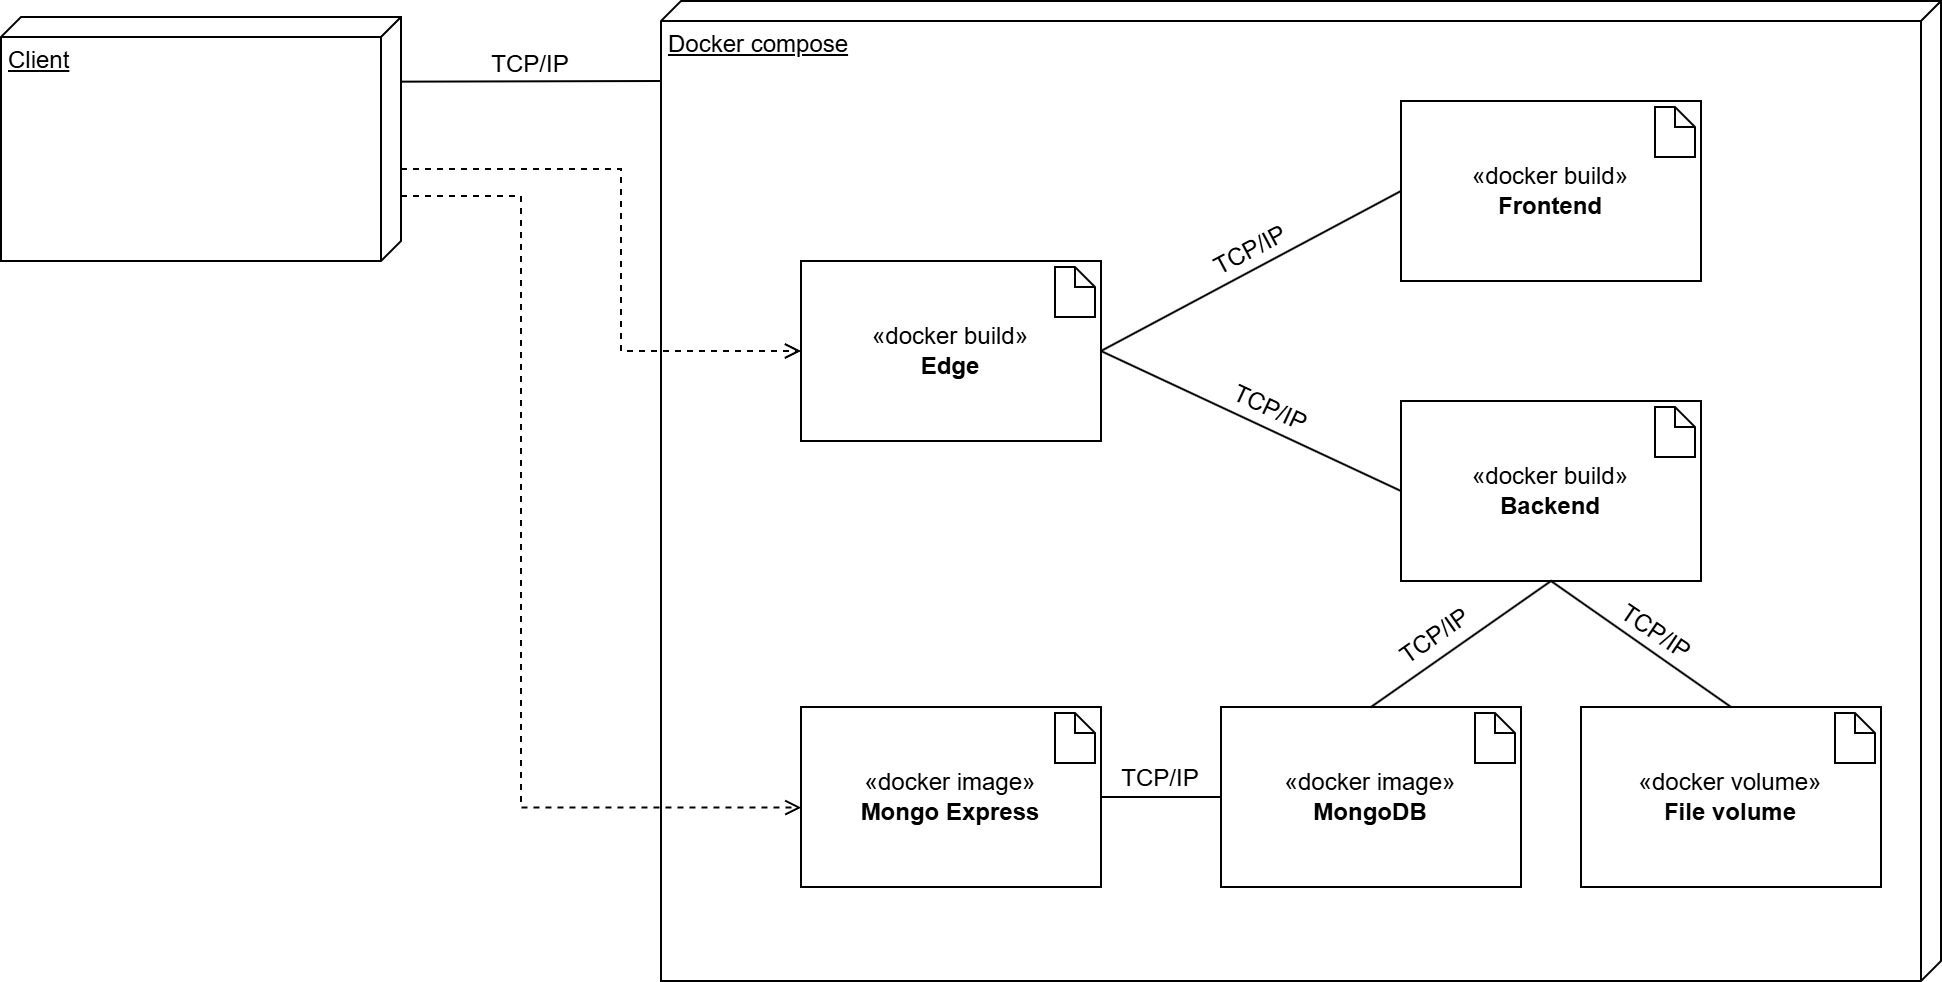
\includegraphics{deployment-diagram-1.png}}
	\caption{Diagram nasazení znázorňující komunikaci přes~TCP/IP protokol aplikace \textit{EDUBO}.}
	\label{fig:deployment-diagram-1}
\end{figure}

Tento diagram nasazení znázorňuje strukturu nasazení aplikace pro~plánování výuky v~prostředí Docker Compose, kde jsou jednotlivé komponenty aplikace rozděleny do~kontejnerů. Kontejnery spolu komunikují pomocí TCP/IP protokolu na~vybraných portech.

Klient představuje zařízení uživatele (např.~počítač nebo mobil), který přistupuje k~aplikaci. Komunikuje s~\textbf{Edge} kontejnerem (NGINX) přes protokol TCP/IP, který zajišťuje směrování požadavků do~backendu nebo frontendu. Správce komunikuje přímo s~kontejnerem \textbf{Mongo Express}, který slouží k~správě databáze MongoDB.

Celý systém je nasazen v~rámci prostředí Docker Compose, které umožňuje spravovat více kontejnerů najednou. V~rámci Docker Compose existuje několik kontejnerů, které plní různé funkce, každý je popsán následovně:

\subsubsection{NGINX}
NGINX je nakonfigurován jako reverzní proxy server. Jeho úkolem je přijímat požadavky od~klienta a~směrovat je na~příslušné komponenty v~rámci aplikace, například do~frontendu nebo backendu. Tento kontejner je sestaven pomocí \texttt{Dockerfile} (v~diagramu vyjádřeno jako stereotyp \textit{<<docker build>>}), což umožňuje přizpůsobit konfiguraci NGINX podle specifických potřeb aplikace (např.~využití Brotli komprese). Komunikuje s~frontendem a~backendem přes TCP/IP a~také zprostředkovává připojení klienta k~Mongo Express a~dalším službám.

\subsubsection{Frontend}
Tato komponenta je zodpovědná za~zobrazení uživatelského rozhraní. Obsahuje kód frontendu aplikace (např.~HTML, CSS, TypeScript) a~je servírována prostřednictvím NGINX. Tento kontejner je sestaven pomocí \texttt{Dockerfile}, aby zahrnoval specifické konfigurace a~balíčky potřebné pro~provoz uživatelského rozhraní. Komunikuje s~NGINX přes TCP/IP protokol, který přijímá požadavky od~klienta a~přesměrovává je do~frontendu.

\subsubsection{Backend}
Backend obsahuje aplikační logiku, která zpracovává požadavky z~frontendu. Je servírován prostřednictvím NGINX a~komunikuje s~dalšími službami (např.~MongoDB). Tento kontejner je sestaven pomocí \texttt{Dockerfile}, což umožňuje nastavit backend tak, aby odpovídal specifickým požadavkům aplikace, včetně požadovaných knihoven a~závislostí. Zajišťuje interakce mezi uživatelskými požadavky (přijatými přes frontend) a~databází, případně dalšími zdroji.

\subsubsection{MongoDB}
MongoDB je dokumentová databáze používaná k~ukládání dat aplikace. Tento kontejner je vytvořen pomocí obrazu z~DockerHubu (v~diagramu vyjádřeno jako stereotyp \textit{<<docker image>>}), což zjednodušuje nasazení databáze bez~nutnosti vlastní konfigurace. Komunikuje s~backendem přes TCP/IP protokol a~poskytuje úložiště pro~data, která jsou uložena ve~formátu Binary JSON (BSON).

\subsubsection{Mongo Express}
Mongo Express je webové rozhraní pro~správu MongoDB, které umožňuje vizuální správu databáze. Běží jako samostatný kontejner a~poskytuje přístup k~MongoDB pro~administrativní účely. Tento kontejner je vytvořen pomocí obrazu z~DockerHubu, což poskytuje rychlý a~snadný způsob pro~správu MongoDB. Komunikuje přímo s~MongoDB pomocí TCP/IP protokolu a~umožňuje správci snadno procházet a~manipulovat s~daty uloženými v~databázi.

\subsubsection{File Volume}
File Volume je úložný prostor pro~soubory, které jsou nahrány do~výukových plánů. Tento objem zajišťuje, že soubory a~data budou uchovány i~při restartu kontejnerů a~slouží jako externí úložiště.

\subsection{Nasazení aplikace Eduklub~--~plány výuky}

\begin{figure}[H]
	\centering
	\resizebox{16cm}{!}{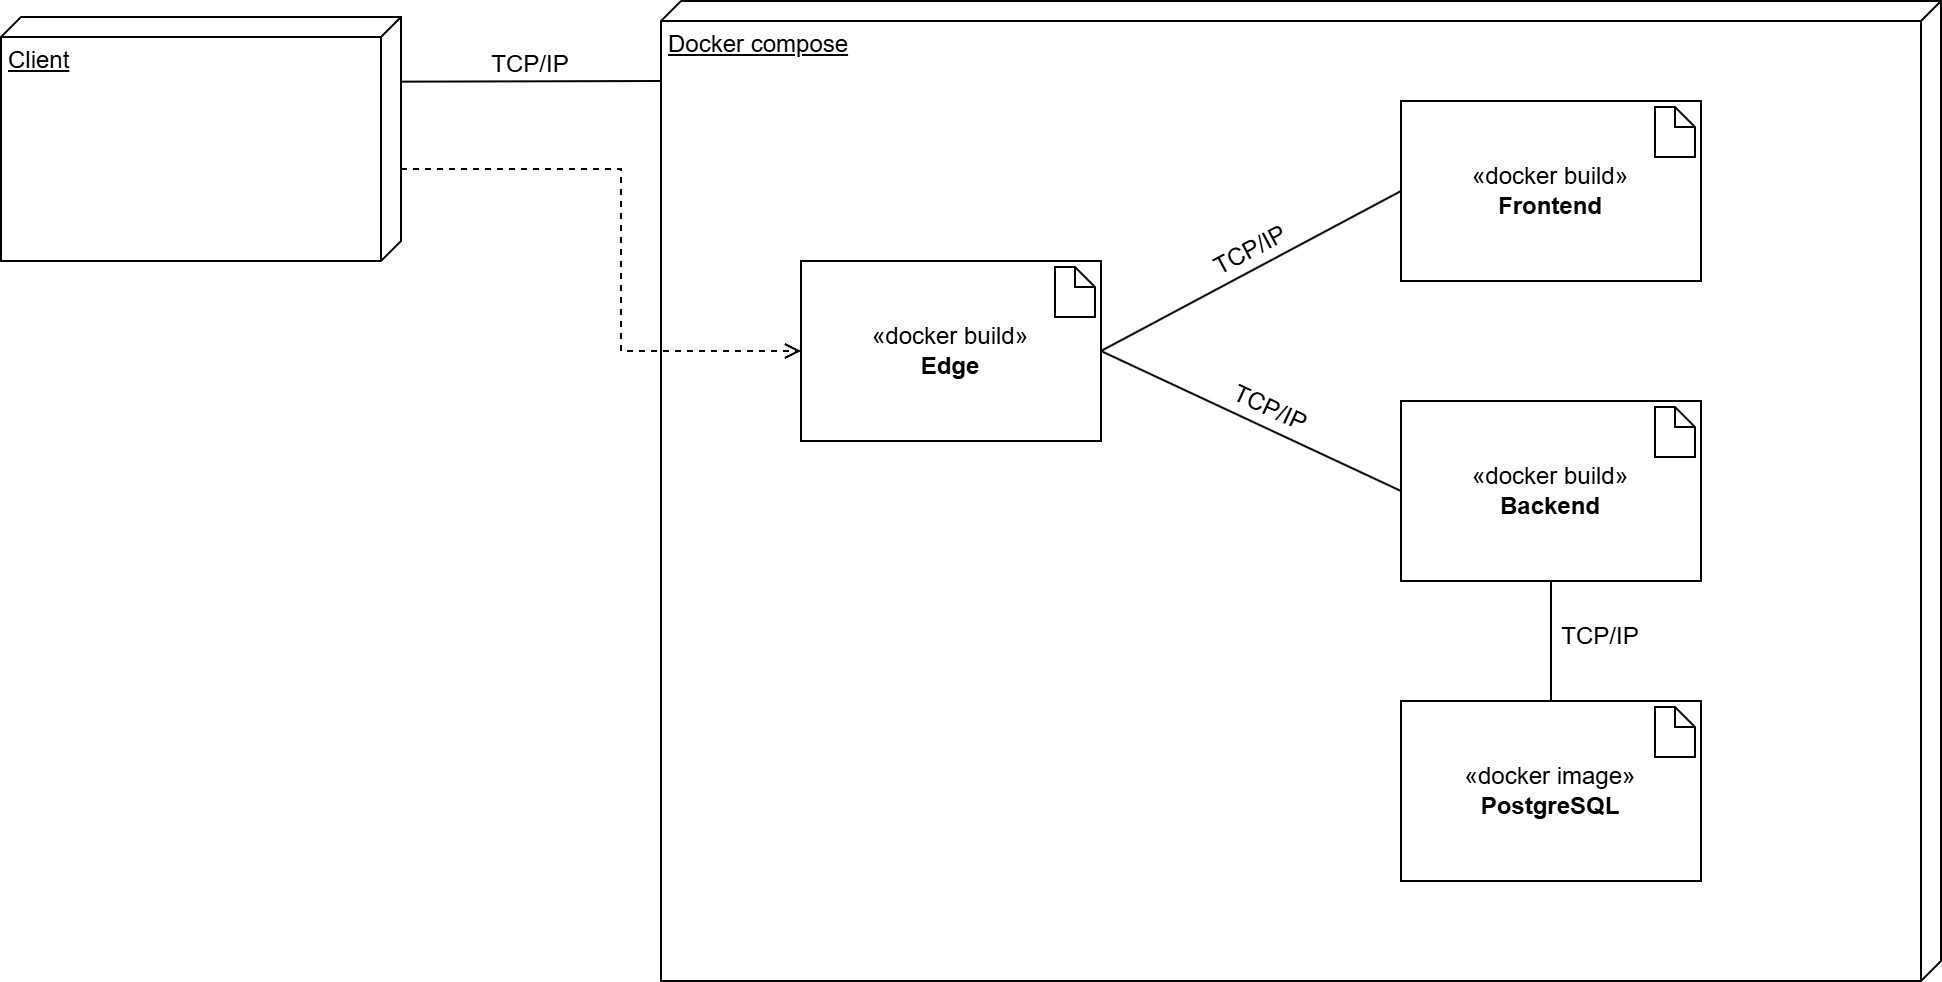
\includegraphics{deployment-diagram-2.png}}
	\caption{Diagram nasazení znázorňující komunikaci přes~TCP/IP protokol aplikace \mbox{\textit{Eduklub~--~plány výuky}.}}
	\label{fig:deployment-diagram-2}
\end{figure}


Tento diagram nasazení znázorňuje nasazení webového agregátoru výukových plánů. Architektura aplikace zůstává téměř shodná s~nasazením \textit{EDUBO}, přičemž jednotlivé komponenty běží v~kontejnerech řízených pomocí Docker Compose. Klient komunikuje s~aplikací přes reverzní proxy server NGINX, který směruje požadavky mezi frontendem a~backendem.

Hlavní změnou oproti~\textit{EDUBO} je nahrazení dokumentové databáze MongoDB relační databází PostgreSQL. Tato změna byla provedena s~cílem efektivnější správy strukturovaných dat a~umožnění komplexnějších dotazů nad výukovými plány, například pro~filtrování mezi sdílenými plány podle různých kritérií, jako je předmět, kategorie nebo klíčová slova. Ostatní komponenty, včetně frontendu, backendu a~jejich vzájemné komunikace, zůstávají stejné.

\subsection{Struktura složek aplikace EDUBO}

\begin{figure}[H]
	\centering
	\resizebox{16cm}{!}{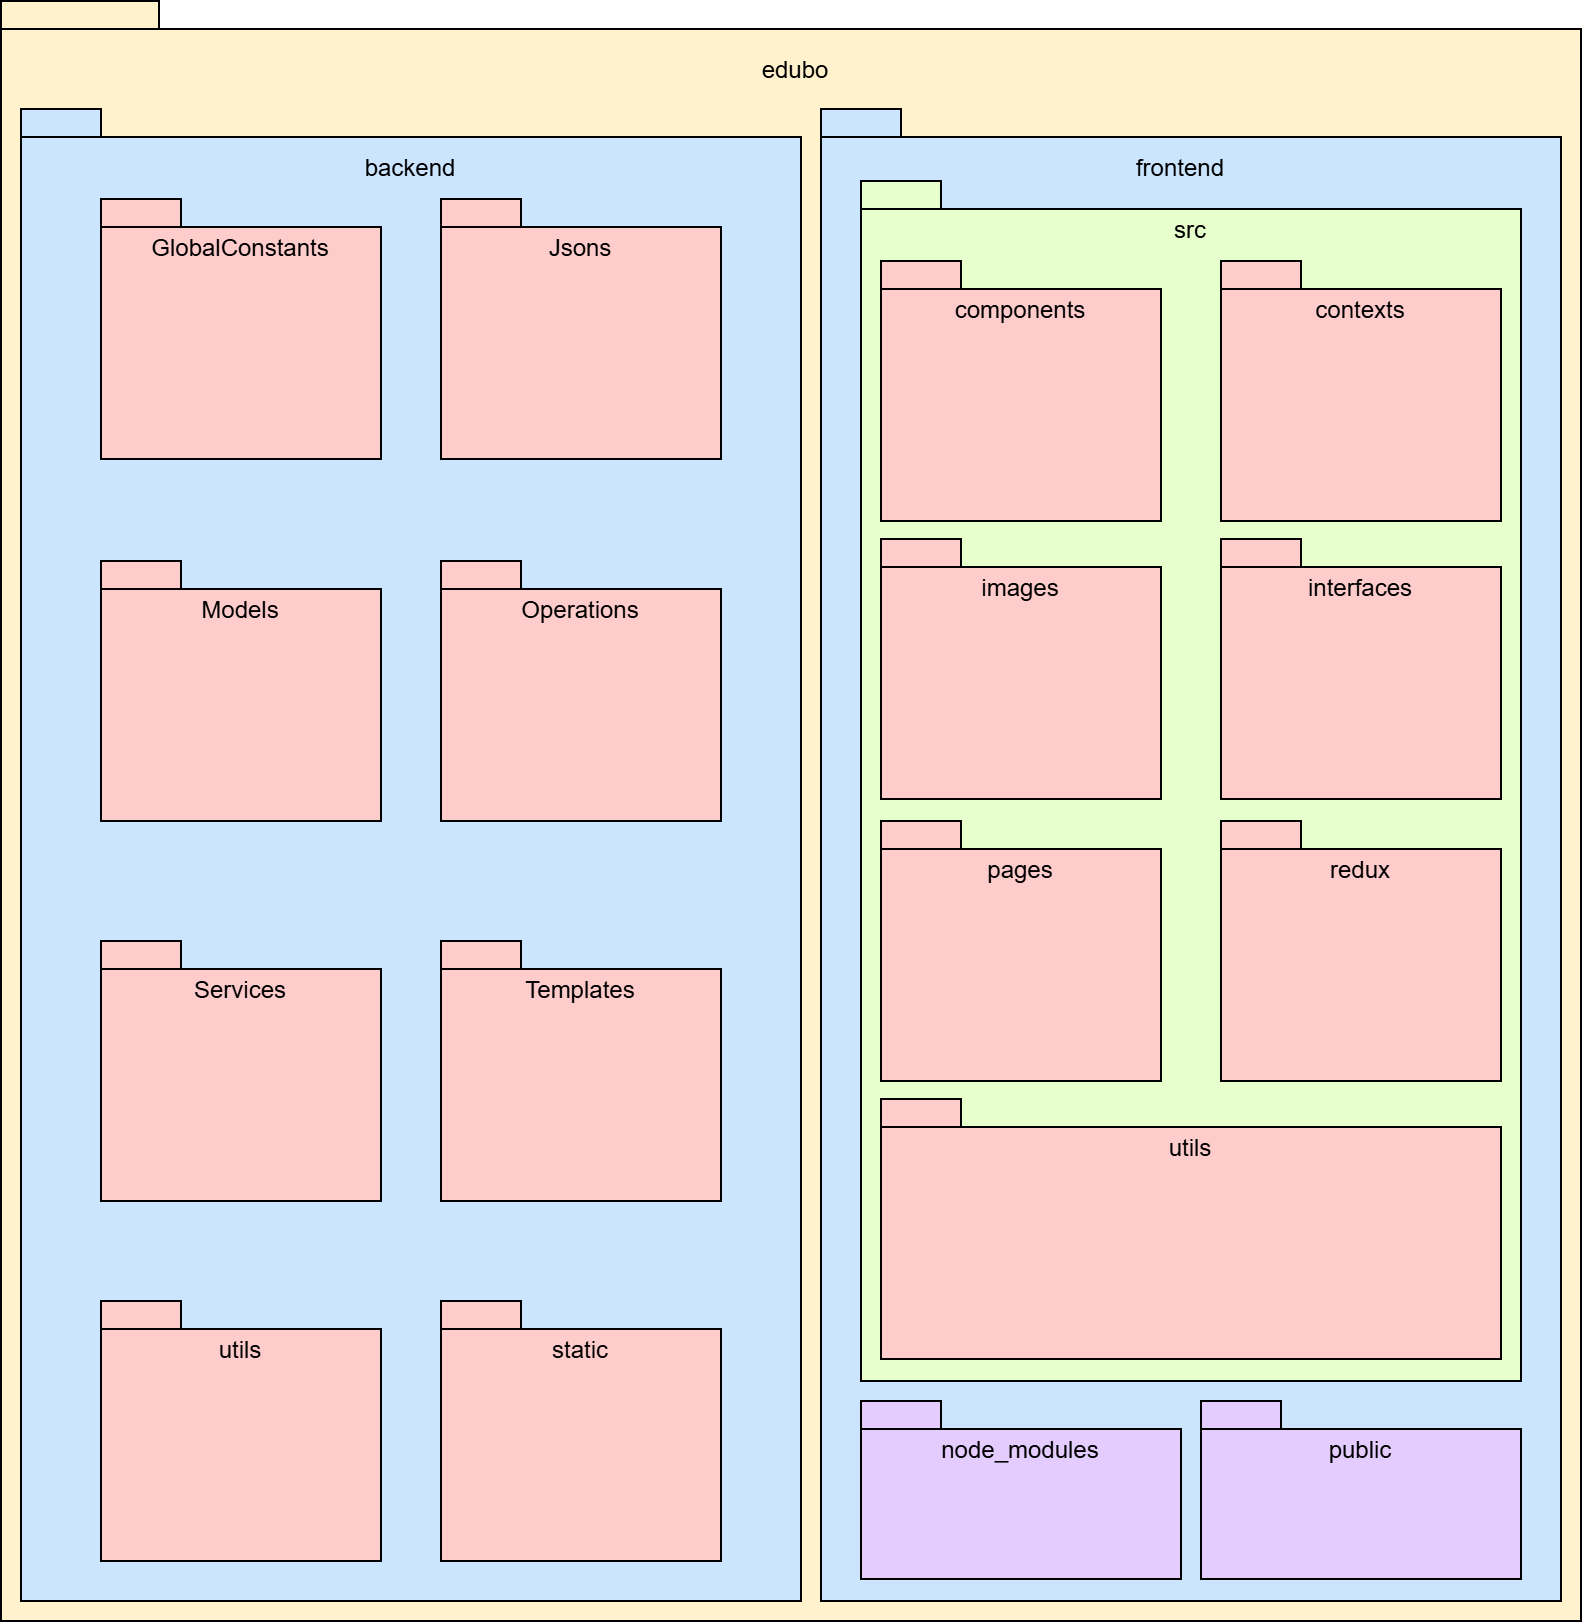
\includegraphics{package-diagram-1.png}}
	\caption{Diagram balíčků znázorňující strukturu složek aplikace \textit{EDUBO}.}
	\label{fig:package-diagram-1}
\end{figure}

Tento diagram balíčků zobrazuje strukturu složek aplikace \textit{EDUBO} postavené na~backendu pomocí Flask (Python) a~frontendu pomocí React (TypeScript). Aplikace je rozdělena do~dvou hlavních částí: \textbf{backend} a~\textbf{frontend}, přičemž každá část obsahuje své specifické složky a~komponenty, které zajišťují určité funkcionality.

\subsubsection{Backend}
\begin{itemize}
	\item \texttt{GlobalConstants}: Tato složka obsahuje globální konstanty, které jsou využívány v~celém backendu. Tyto konstanty zahrnují nastavení aplikace, konfigurace nebo klíčové proměnné, které jsou sdíleny mezi jednotlivými moduly.
	\item \texttt{Jsons}: Složka obsahuje příkladné JSON soubory, které ukazují, jak vypadají datové struktury typů aktivit, výukového plánu, kurikulárních výstupů a~uživatelských dat.
	\item \texttt{Models}: Obsahuje Pydantic modely a~Marshmallow schémata, které definují strukturu a~validaci dat.
	\item \texttt{Operations}: Tato složka zahrnuje databázové operace, tedy CRUD (Create, Read, Update, Delete) operace pro~MongoDB. Každá operace je implementována jako funkce, která interaguje s~databází a~umožňuje manipulaci s~uloženými daty.
	\item \texttt{Services}: Obsahuje API endpointy, které jsou definovány pomocí Flask blueprintů. Tyto služby fungují podobně jako views v~Djangu, kde každý service odpovídá určitému API endpointu a~zpracovává konkrétní typ požadavku (např.~GET, POST). Blueprinty v~této složce rozdělují logiku aplikace na~menší, modulární části, což usnadňuje správu a~rozšiřování kódu.
	\item \texttt{Templates}: Složka pro~šablony určené k~vykreslení PDF dokumentů, konkrétně plánů výuky. Obsahuje Jinja2 kód, který se generuje jako HTML výstup, který si mohou uživatelé stáhnout nebo vytisknout ve~formě PDF.
	\item \texttt{utils}: Obsahuje pomocné utility, což mohou být například funkce nebo skripty, které usnadňují opakované operace napříč aplikací. Tyto utility zahrnují formátování dat, konverze nebo jiné malé pomocné operace.
	\item \texttt{static}: Slouží k~ukládání statických souborů, jako jsou obrázky, styly (CSS) nebo JavaScript, které jsou nezávislé na~dynamicky generovaném obsahu aplikace.
\end{itemize}

\subsubsection{Frontend}
\begin{itemize}
	\item \texttt{src}:
	\begin{itemize}
		\item \texttt{components}: Obsahuje React komponenty, které tvoří jednotlivé části uživatelského rozhraní. Tyto komponenty slouží v~systému jako znovupoužitelné prvky, například tlačítka, formuláře nebo karty, které se skládají dohromady, aby vytvořily plné stránky aplikace.
		\item \texttt{contexts}: Obsahuje kontexty pro~React, což jsou data, která lze sdílet napříč komponentami.
		\item \texttt{images}: Složka pro~ukládání obrázků používaných v~uživatelském rozhraní, jako jsou loga, ikony nebo ilustrace.
		\item \texttt{interfaces}: Závazky pro~TypeScript, které definují struktury dat používané v~aplikaci. Používají se k~zajištění typové bezpečnosti při práci s~daty.
		\item \texttt{pages}: Obsahuje jednotlivé stránky aplikace (např.~Přihlášení, Registrace, Editor). Každá stránka je tvořena kombinací komponent a~zobrazuje konkrétní obsah aplikace.
		\item \texttt{redux}: Obsahuje konfigurace a~reducery pro~Redux, což je knihovna pro~správu stavu aplikace.
		\item \texttt{utils}: Stejně jako na~backendu, tato složka obsahuje pomocné funkce, které se používají napříč frontendem. Jsou zde například funkce pro~formátování dat.
		\item \texttt{node\_modules}: Tato složka obsahuje všechny závislosti a~knihovny nainstalované pomocí Node.js. Je automaticky generována při instalaci balíčků a~obsahuje knihovny třetích stran.
		\item \texttt{public}: Složka pro~veřejné soubory, které jsou přístupné přímo z~prohlížeče\break(např.~favicon, \texttt{index.html}). Tyto soubory jsou statické a~nemění se během běhu aplikace.
	\end{itemize}
\end{itemize}

\subsection{Struktura složek Eduklub~--~plány výuky}

\begin{figure}[H]
	\centering
	\resizebox{16cm}{!}{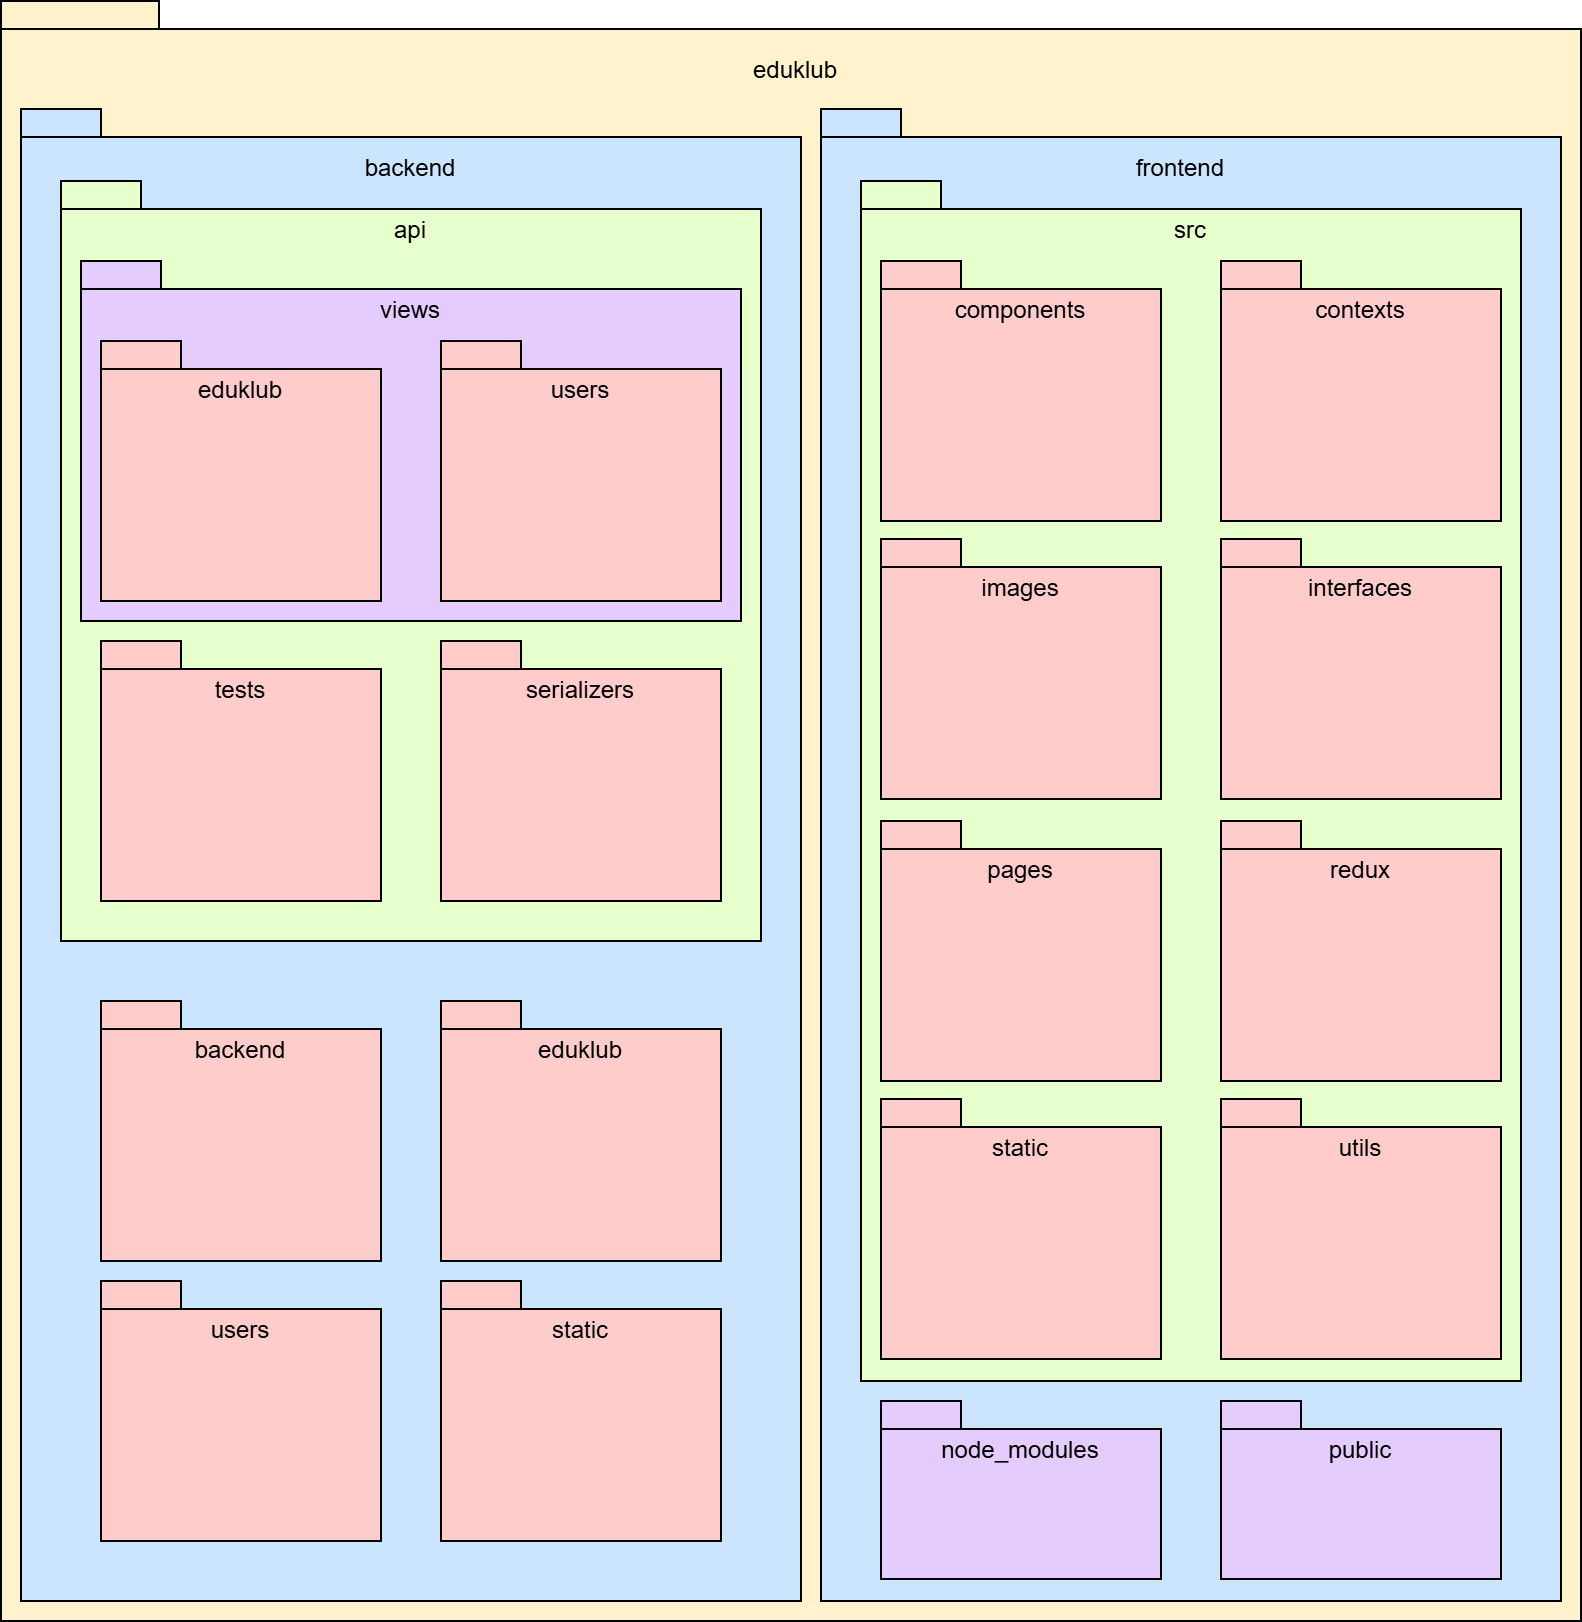
\includegraphics{package-diagram-2.png}}
	\caption{Diagram balíčků znázorňující strukturu složek aplikace \textit{Eduklub~--~plány výuky}.}
	\label{fig:package-diagram-2}
\end{figure}

\needspace{4\baselineskip}
Tento diagram balíčků zobrazuje strukturu složek webové agregátoru výukových plánů, kde je backend vytvořen pomocí Django (Python) a~frontend pomocí React (TypeScript). Diagram ukazuje hlavní složky a~jejich účel, což poskytuje přehled o~architektuře aplikace. Struktura frontendových složek je v~package diagramu shodná se~strukturou použitou v~\textit{EDUBO}.

\subsubsection{Backend}

\begin{itemize}
	\item \texttt{api}: Obsahuje strukturu pro~API aplikace, která je rozdělena na~jednotlivé části zajišťující různé funkce aplikace.
	\item \texttt{views}:
	\begin{itemize}
		\item \texttt{eduklub}: Obsahuje views pro~hlavní funkce aplikace, které zajišťují zpracování požadavků týkajících se~obsahu a~funkcí platformy.
		\item \texttt{users}: Obsahuje views specifické pro~správu uživatelů, například autentizaci, registraci a~správu uživatelských profilů.
	\end{itemize}
	\item \texttt{serializers}: Obsahuje serializéry, které převádějí data mezi Django modely a~JSON formátem.
	\item \texttt{tests}: Obsahuje testy pro~jednotlivé části API, které slouží k~ověření funkčnosti~implementace.
	\item \texttt{backend}: Obsahuje hlavní konfigurační soubory a~nastavení specifické pro~backend aplikace. Může obsahovat například nastavení databáze, middleware nebo bezpečnostní konfigurace.
	\item \texttt{eduklub}: Tato složka obsahuje modely všech objektů kromě uživatelů.
	\item \texttt{users}: Složka pro~správu uživatelských účtů a~uživatelských modelů. Obsahuje funkce pro~autentizaci, autorizaci a~správu profilů.
	\item \texttt{static}: Obsahuje statické soubory potřebné pro~backend, například styly, JavaScript nebo obrázky.
\end{itemize}

\subsection{Databázové schéma aplikace EDUBO}

\needspace{9\baselineskip}
V~systému se nachází následující entity:
\begin{itemize}
	\item Uživatel~--~osoba, která pracuje s~aplikací. Může to být učitel, žák nebo rodič.
	\item Třída~--~organizační jednotka, ke~které jsou přiřazeni žáci a~učitelé.
	\item Předmět~--~oblast výuky (např.~matematika, čeština), k~níž jsou přiřazeny výukové celky.
	\item Výukový celek~--~sada tematicky souvisejících výukových plánů.
	\item Výukový plán~--~konkrétní plán jedné vyučovací jednotky.
	\item Aktivita~--~základní stavební prvek výukového plánu, který definuje konkrétní činnost (např.~diskuse, práce s~textem, test).
\end{itemize}

\begin{figure}[H]
	\centering
	\resizebox{16cm}{!}{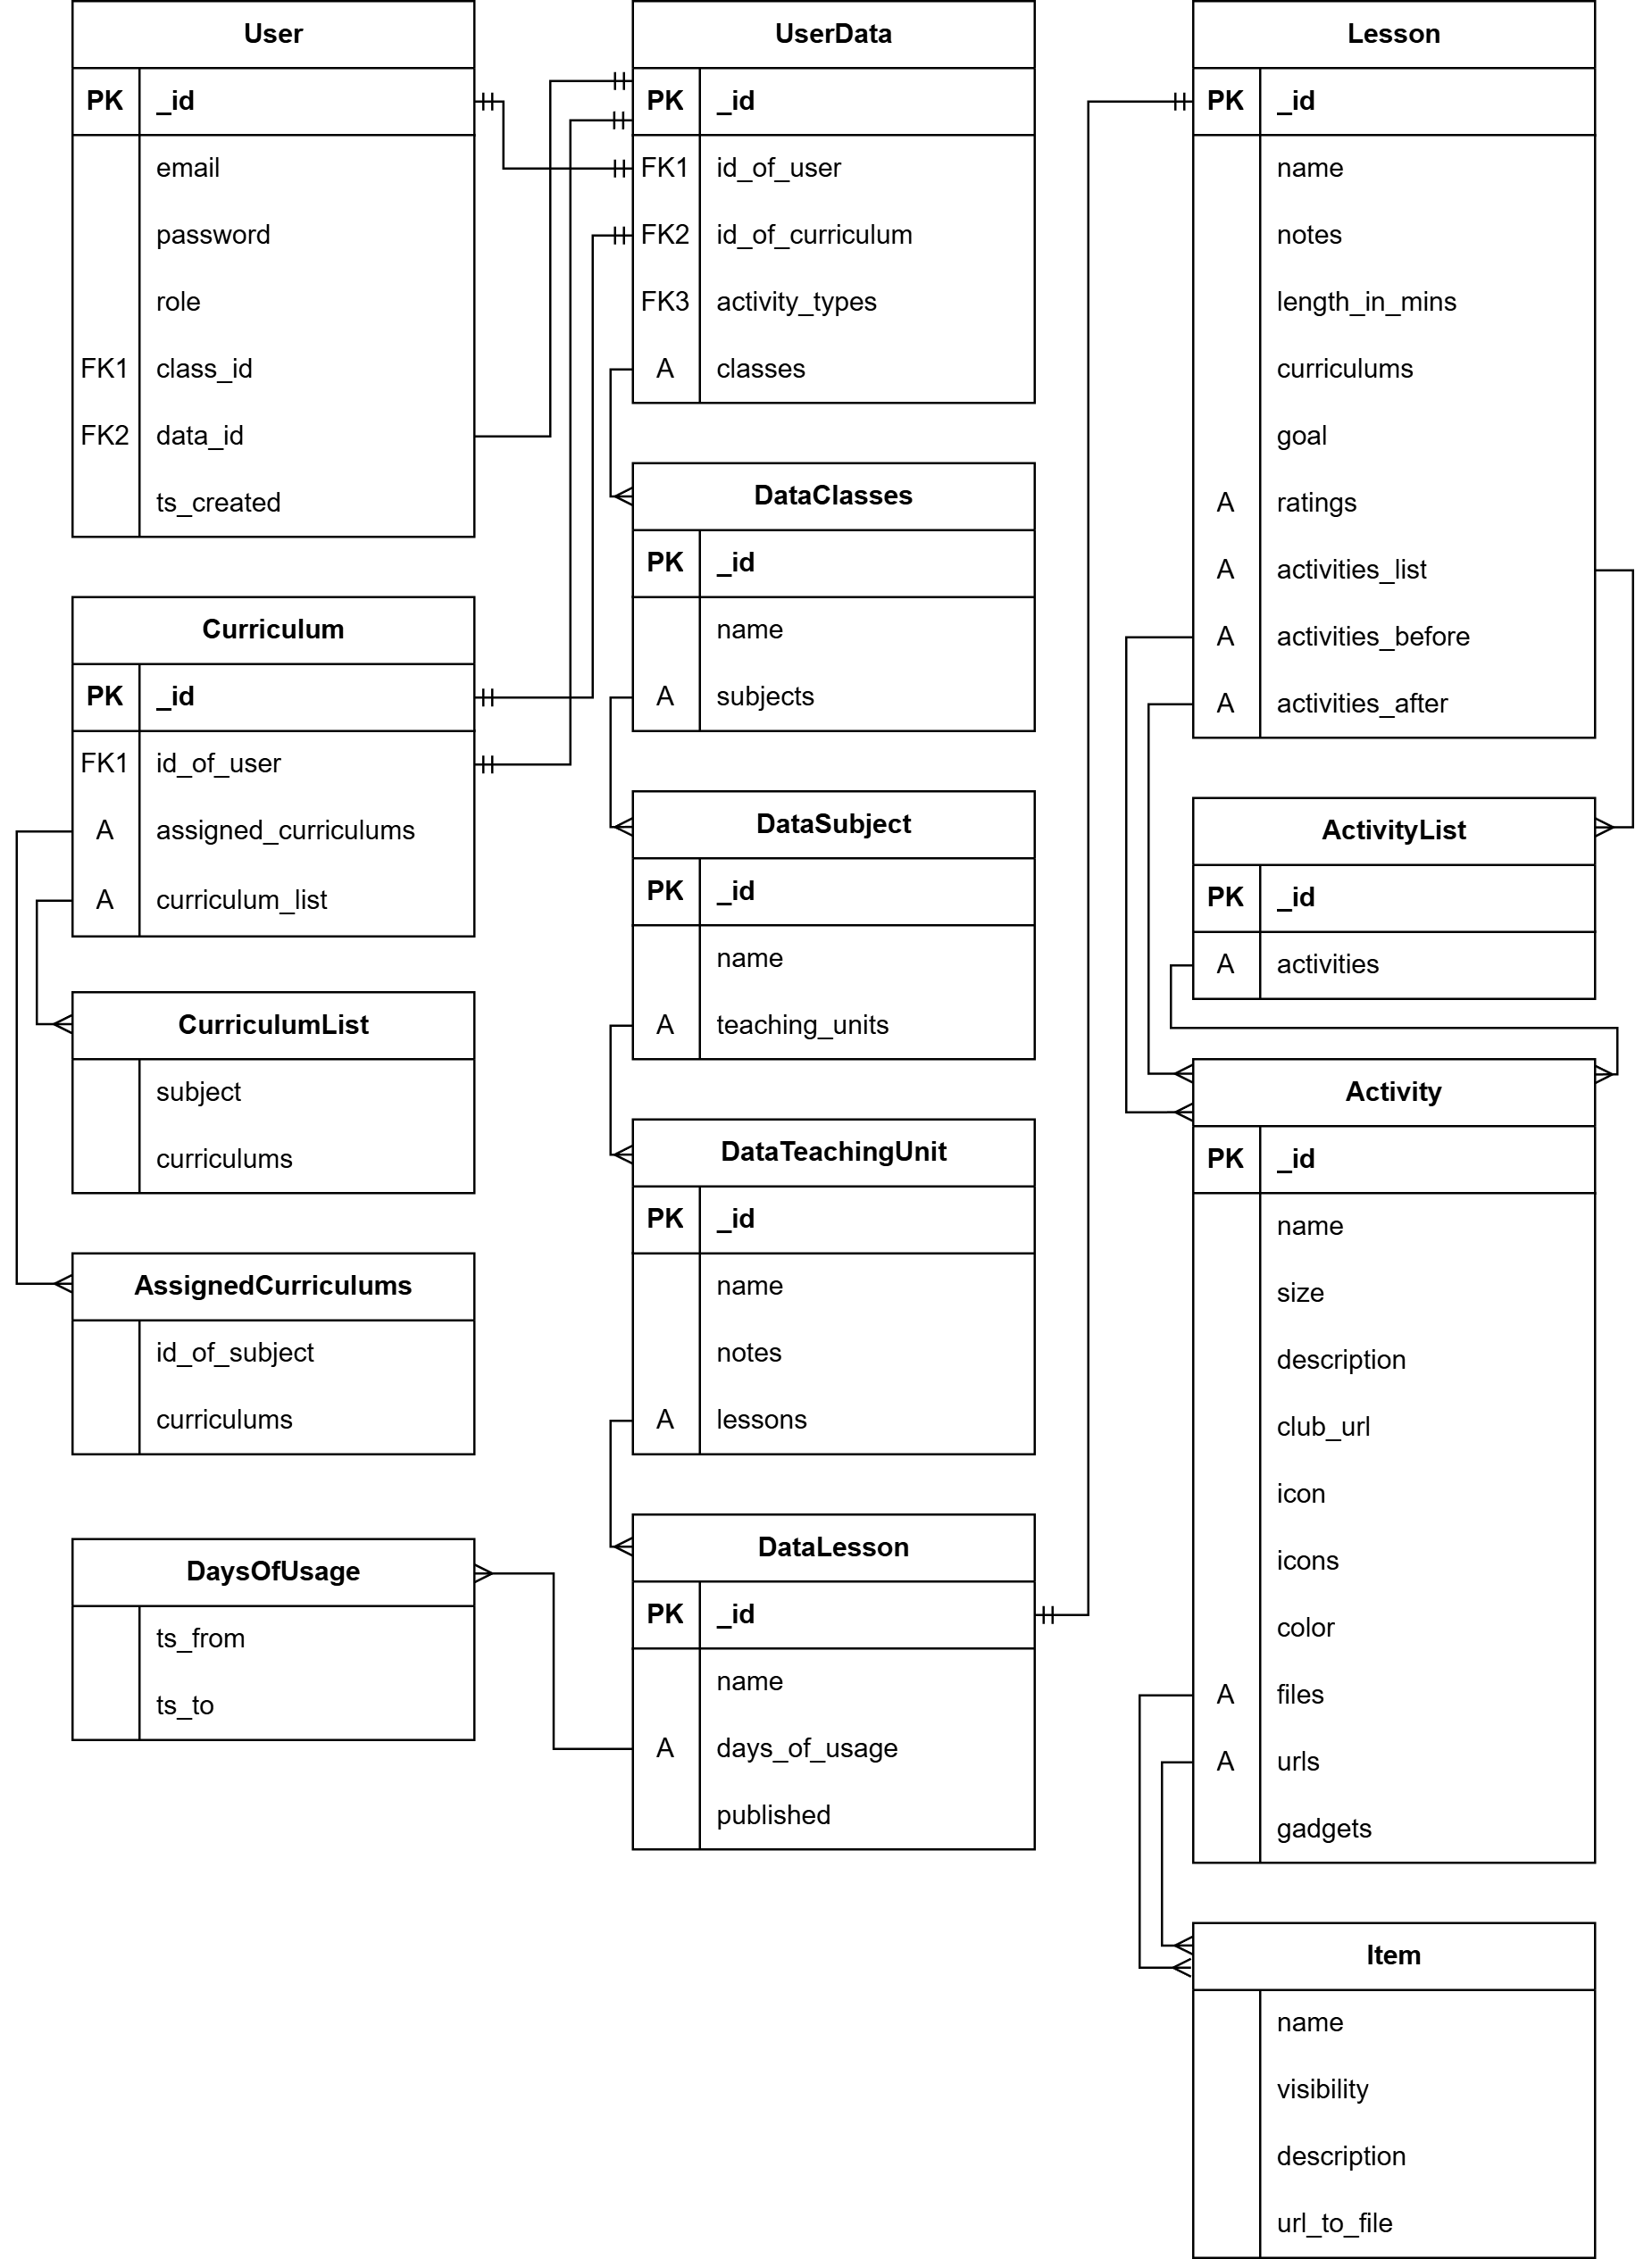
\includegraphics{erd-1.png}}
	\caption{Entitně-vztahový diagram znázorňující databázovou strukturu aplikace \textit{EDUBO}.}
	\label{fig:erd-1}
\end{figure}

Tento entitně-vztahový diagram popisuje databázovou strukturu pro aplikaci \textit{EDUBO}. Diagram je navržen specificky pro dokumentovou databázi, kde některé tabulky fungují jako objekty s~poli dalších podobjektů. Šipky s~vidlicí vedoucí přímo do názvu tabulky označují podtabulky (pole objektů), což znamená, že pokud má záznam v~prvním sloupci \quotedblbase A``, odkazuje na pole těchto objektů. Tento diagram není kompletní a~chybí zde šest tabulek (\texttt{Class}, \texttt{ClassKey}, \texttt{ParentKey}, \texttt{ActivityTypes}, \texttt{ActivityTypeList}, \texttt{Rating}) a~to kvůli čitelnosti. Kompletní diagram se nachází v~externí příloze. Diagram zajišťuje organizaci dat týkajících se~uživatelů, dat učitelů a~výukových plánů.

\textbf{Popis důležitých objektů:}
\begin{itemize}
	\item \texttt{User:} Obsahuje základní informace o~uživatelích systému.
	\begin{itemize}
		\item \texttt{role}~--~Role uživatele v~systému (student, teacher nebo parent).
		\item \texttt{data\_id}~--~Odkaz na~objekt v~tabulce \texttt{UserData}, který obsahuje podrobné informace o~uživateli.
	\end{itemize}
	
	\item \texttt{Curriculum:} Tabulka, která obsahuje přiřazené kurikulární výstupy k~předmětům.
	\begin{itemize}
		\item \texttt{assigned\_curriculums}~--~Pole přiřazených kurikulárních výstupů k~předmětům. 
		\\\texttt{id\_of\_subject}, \texttt{curriculums}: Výčet výstupů, které učitel přiřadil k~danému předmětu.
		\item \texttt{curriculum\_list}~--~Výchozí a~vlastní nahrané výstupy, které uživatel může přiřadit ke~svým předmětům.
		\\\texttt{subject}, \texttt{curriculums}: Název předmětu a~výstupy pro~daný předmět.
	\end{itemize}
	
	\item \texttt{UserData:} Obsahuje podrobné informace o~uživateli.
	\begin{itemize}
		\item \texttt{classes}~--~Seznam tříd, ke~kterým je uživatel přiřazen.
		\\Každá třída obsahuje:
		\item \texttt{subjects}~--~Pole předmětů vyučovaných v~dané třídě.
		\\Každý předmět obsahuje:
		\item \texttt{name}~--~Název předmětu.
		\item \texttt{teaching\_units}~--~Výukové celky, které daný předmět obsahuje.
		\\Každý výukový celek obsahuje:
		\item \texttt{notes}~--~Poznámky k~výukovému celku.
		\item \texttt{lessons}~--~Seznam výukových plánů.
		\\Každý výukový plán obsahuje:
		\item \texttt{published}~--~Příznak publikace výukového plánu.
		\item \texttt{days\_of\_usage}~--~Termíny, kdy byl výukový plán použit.
	\end{itemize}
	
	\needspace{16\baselineskip}
	\item \texttt{Lesson:} Obsahuje informace o~jednotlivých výukových plánech.
	\begin{itemize}
		\item \texttt{name}~--~Název výukového plánu.
		\item \texttt{notes}~--~Poznámky k~výukovému plánu.
		\item \texttt{length\_in\_mins}~--~Délka trvání výukového plánu v~minutách.
		\item \texttt{curriculums}~--~Přiřazené kurikulární výstupy.
		\item \texttt{goal}~--~Vzdělávací cíl výukového plánu.
		\item \texttt{activities\_list}~--~Pole paralelních aktivit, které se~realizují během výuky.
		\\Každé pole obsahuje \texttt{activities}, což jsou pole, které obsahují samotné aktivity.
		\item \texttt{activities\_before}, \texttt{activities\_after}~--~Pole aktivit před nebo po~hodině.
		\\Každá aktivita obsahuje:
		\item \texttt{name}, \texttt{size}, \texttt{description}, \texttt{icons}, \texttt{color}~--~Základní informace.
		\item \texttt{club\_url}~--~Odkaz na~související metodické materiály na~platformě Eduklub.
		\item \texttt{gadgets}~--~Pomůcky využívané během aktivity.
		\item \texttt{files}, \texttt{urls}~--~Soubory a~odkazy připojené k~aktivitě.
		\\Každý soubor/odkaz zahrnuje:
		\item \texttt{name}, \texttt{visibility}, \texttt{description}, \texttt{url\_to\_file}~--~Základní informace.
	\end{itemize}
\end{itemize}

\newpage % TODO: SMAZAT???? %

\begin{lstlisting}
class ExtendedItems(Schema):
 name = fields.String(validate=validate.Length(max=1023))
 visibility = fields.String(validate=validate.OneOf(["student", "teacher", "after-lesson"]))
 description = fields.String(validate=validate.Length(max=1023))
 url_to_file = fields.String()

class ActivitySchema(Schema):
 _id = fields.String(validate=validate.Length(equal=36))
 name = fields.String(validate=validate.Length(max=127))
 size = fields.Integer(validate=validate.Range(min=1))
 description = fields.String(validate=validate.Length(max=8191))
 club_url = fields.String()
 icon = fields.String(validate=validate.OneOf(["xxx"]))
 icons = fields.List(fields.String(validate=validate.OneOf(["xxx"])))
 color = fields.String(validate=validate.Length(equal=7))
 files = fields.List(fields.Nested(ExtendedItems))
 urls = fields.List(fields.Nested(ExtendedItems))
 gadgets = fields.List(fields.String(validate=validate.Length(max=255)))
	
class ActivityList(Schema):
 _id = fields.String(validate=validate.Length(equal=36))
 activities = fields.List(fields.Nested(ActivitySchema))
	
class Rating(Schema):
 id_of_user = fields.String()
 rating = fields.String(validate=validate.OneOf(["downvote", "upvote", "neutral", "unused"]))
	
class LessonDatabaseSchema(Schema):
 _id = fields.String(validate=validate.Length(equal=36))
 ts_created = fields.String()
 ts_updated = fields.String()
 name = fields.String(validate=validate.Length(max=68))
 notes = fields.String(validate=validate.Length(max=4095))
 length_in_mins = fields.Integer(validate=validate.Range(min=5, max=720))
 curriculums = fields.List(fields.String)
 goal = fields.String(validate=validate.Length(max=511))
 ratings = fields.List(fields.Nested(Rating))
 activities_list = fields.List(fields.Nested(ActivityList))
 activities_before = fields.List(fields.Nested(ActivitySchema))
 activities_after = fields.List(fields.Nested(ActivitySchema))
\end{lstlisting}

Toto schéma definuje strukturu výukového plánu pomocí ORM (Objektově-relační mapování) knihovny Marshmallow v~jazyce Python. Každá lekce je reprezentována třídou\break\texttt{LessonDatabaseSchema}, která obsahuje klíčové informace, jako je název, čas vytvoření, poznámky a~délka lekce. Lekce může mít přiřazené kurikulární výstupy a~definovaný cíl. Klíčovou součástí schématu je seznam aktivit, který je strukturován do~tří hlavních částí~--~běžné aktivity v~hodině (\texttt{activities\_list}), aktivity před hodinou (\texttt{activities\_before}) a~aktivity po hodině (\texttt{activities\_after}). Každá aktivita (\texttt{ActivitySchema}) má své unikátní ID, název, popis, velikost a~další atributy, jako je barva, soubory, URL odkazy a~pomůcky.

Další částí modelu je hodnocení výukových plánů, které je reprezentováno třídou \texttt{Rating}. Každý žák může označit lekci jako pozitivní, negativní, neutrální nebo ji neohodnotit. Pro~správu souborů a~odkazů byla vytvořena samostatná struktura \texttt{ExtendedItems}, která určuje viditelnost těchto položek (pro~studenty, učitele nebo po~hodině).

\subsection{Databázové schéma aplikace Eduklub~--~plány výuky}

\begin{figure}[H]
	\centering
	\resizebox{16cm}{!}{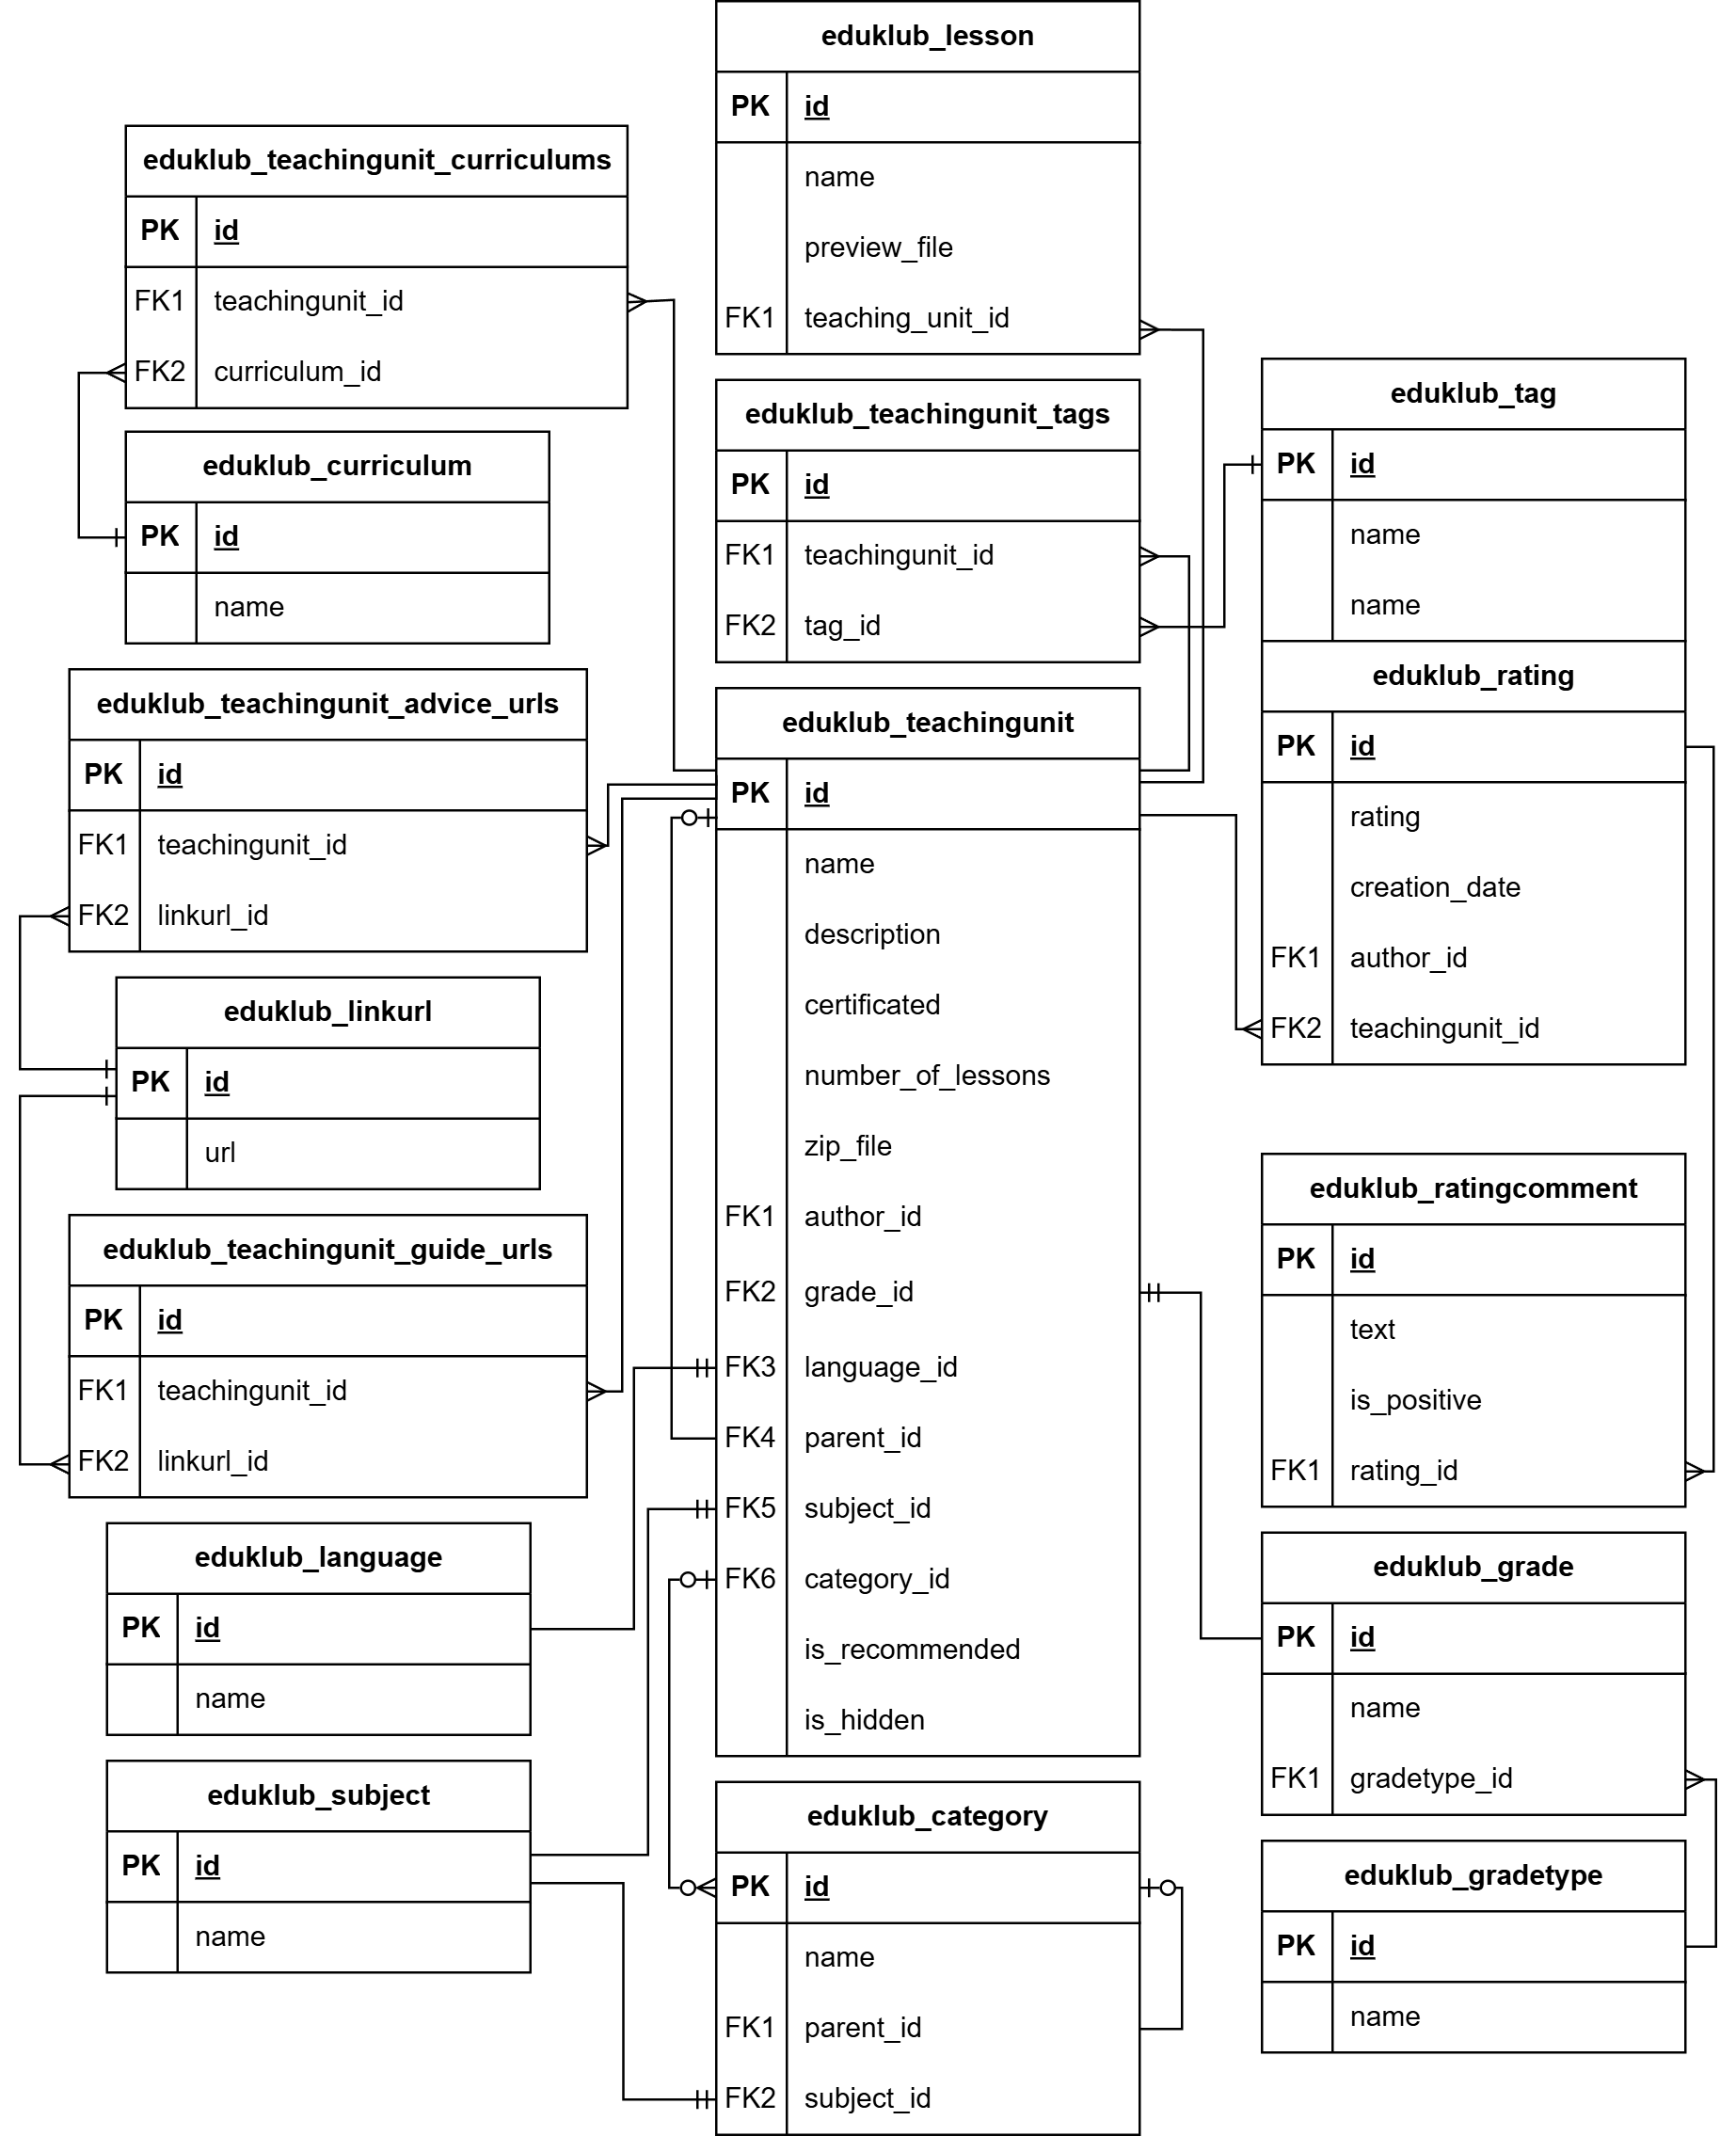
\includegraphics{erd-2.png}}
	\caption{Entitně-vztahový diagram znázorňující databázovou strukturu aplikace \mbox{\textit{Eduklub~--~plány výuky}.}}
	\label{fig:erd-2}
\end{figure}

Tento entitně-vztahový diagram popisuje databázovou strukturu pro webový agregátor výukových plánů. Diagram není kompletní a~chybí zde tři tabulky (\texttt{favoritelist\_teaching\_units}, \texttt{user}, \texttt{favoritelist}) z~důvodu úspory místa v~textu této závěrečné práce. Kompletní diagram se~nachází v~externí příloze.

Popis důležitých tabulek:
\begin{itemize}
	\item \textbf{eduklub\_teachingunit}: Centrální tabulka pro výukové celky v~aplikaci.
	\begin{itemize}
		\item \texttt{name}, \texttt{description}: Název a~popis výukového celku.
		\item \texttt{certificated}: Příznak určující, zda je plán certifikovaný.
		\item \texttt{number\_of\_lessons}: Počet výukových hodin ve~výukovém celku.
		\item \texttt{author\_id}: Odkaz na~uživatele, který jednotku vytvořil.
		\item \texttt{grade\_id}: Ročník, do~kterého výukový celek spadá.
		\item \texttt{parent\_id}: Odkaz na~rodičovský celek, pokud se~jedná o~mutaci jiného celku.
		\item \texttt{subject\_id}: Předmět, do~které výukový celek spadá.
		\item \texttt{category\_id}: Kategorie, do~které výukový celek spadá. Tabulka \texttt{eduklub\_category} obsahuje \texttt{subject\_id}. Tento vztah umožňuje existenci kategorií i~bez přiřazení konkrétního výukového celku, což je nezbytné pro robustní filtrovací systém aplikace. Výukový celek nemusí být přiřazen k~žádné kategorii, ale vždy spadá pod předmět.
		
	\end{itemize}
	
	\item \textbf{eduklub\_lesson}: Tabulka pro jednotlivé výukové hodiny, které jsou součástí výukových celků.
	\begin{itemize}
		\item \texttt{name}: Název výukové hodiny.
		\item \texttt{preview\_file}: Náhledový HTML soubor výukové hodiny.
		\item \texttt{teachingunit\_id}: Odkaz na~výukový celek, ke~kterému výuková hodina patří.
	\end{itemize}
	
	\item \textbf{eduklub\_category}: Tabulka pro kategorie výukových celků.
	\begin{itemize}
		\item \texttt{name}: Název kategorie.
		\item \texttt{parent\_id}: Možnost hierarchického uspořádání kategorií.
	\end{itemize}
	
	\item \textbf{eduklub\_tag}: Tabulka pro značky, které lze přiřadit výukovým celkům.
	
	\item \textbf{eduklub\_rating}: Tabulka pro hodnocení výukových celků.
	\begin{itemize}
		\item \texttt{rating}: Hodnota hodnocení.
		\item \texttt{creation\_date}, \texttt{author\_id}: Datum vytvoření a~odkaz na~uživatele, který hodnocení vytvořil.
	\end{itemize}
	
	\item \textbf{eduklub\_ratingcomment}: Obsahuje komentáře k~hodnocením.
	\begin{itemize}
		\item \texttt{id}, \texttt{text}: Primární klíč a~text komentáře.
		\item \texttt{is\_positive}: Příznak indikující, zda je komentář pozitivní.
		\item \texttt{rating\_id}: Odkaz na~hodnocení, ke~kterému komentář patří.
	\end{itemize}
	
	\item \textbf{eduklub\_gradetype}: Typ vzdělávacího stupně, který poskytuje specifikaci pro jednotlivé ročníky v~tabulce \texttt{eduklub\_grade}. Například 1.~stupeň základní školy.
	\begin{itemize}
		\item \texttt{id}, \texttt{name}: Primární klíč a~název typu ročníku.
	\end{itemize}
	
	\item \textbf{eduklub\_grade}: Obsahuje ročníky ze~vzdělávacích stupňů, pro~které je výukový celek určen.
	\begin{itemize}
		\item \texttt{name}, \texttt{grade\_type\_id}: Název ročníku a~odkaz na~typ ročníku.
	\end{itemize}
\end{itemize}

\begin{lstlisting}
 class TeachingUnit(models.Model):
   name = models.CharField(max_length=63)
   description = models.TextField(null=True, blank=True)
   certificated = models.BooleanField(default=False)
   is_recommended = models.BooleanField(default=False)
   creation_date = models.DateField(auto_now_add=True)
   is_hidden = models.BooleanField(default=False)
   number_of_lessons = models.IntegerField()
   number_of_downloads = models.IntegerField(default=0)
   zip_file = models.FileField(upload_to='teaching_units/zip_files')
   language = models.ForeignKey(Language, on_delete=models.PROTECT)
   author = models.ForeignKey(User, on_delete=models.PROTECT, null=True)
   tags = models.ManyToManyField(Tag, related_name='teaching_units', blank=True)
   parent = models.ForeignKey('self', on_delete=models.PROTECT, null=True, blank=True)
   alternatives = models.ManyToManyField('self', blank=False)
   advice_urls = models.ManyToManyField(LinkURL, related_name='advice_urls', blank=True)
   guide_urls = models.ManyToManyField(LinkURL, related_name='guide_urls', blank=True)
   subject = models.ForeignKey(Subject, on_delete=models.PROTECT)
   grade = models.ForeignKey(Grade, on_delete=models.PROTECT)
   curriculums = models.ManyToManyField(Curriculum, related_name='teaching_units', blank=True)
   category = models.ForeignKey(Category, on_delete=models.PROTECT, null=True, blank=True)
	
  class Lesson(models.Model):
    name = models.CharField(max_length=63)
    preview_file = models.FileField(upload_to='lessons/preview_files')
    teaching_unit = models.ForeignKey(TeachingUnit, on_delete=models.CASCADE, related_name='lessons')
	
  class Category(models.Model):
    name = models.CharField(max_length=63)
    parent = models.ForeignKey('self', on_delete=models.PROTECT, null=True, blank=True, related_name='children')
    subject = models.ForeignKey(Subject, on_delete=models.PROTECT, blank=True, null=True)
\end{lstlisting}

Toto schéma definuje strukturu výukového celku a~jeho jednotlivých lekcí pomocí ORM Django. \texttt{TeachingUnit} reprezentuje výukový celek s~atributy jako název, popis, počet lekcí a~soubor ke~stažení. Každý výukový celek může mít rodičovský celek (\texttt{parent}), což umožňuje vytváření mutací. \texttt{Lesson} představuje jednotlivé lekce a~obsahuje soubor náhledu ve~formátu HTML. \texttt{Category} pak slouží k~tematickému zařazení výukových celků. Kategorie mohou být hierarchicky uspořádané pomocí vazby \texttt{parent}, což umožňuje vytvářet nadřazené a~podřazené skupiny.

\begin{figure}[H]
	\centering
	\resizebox{16cm}{!}{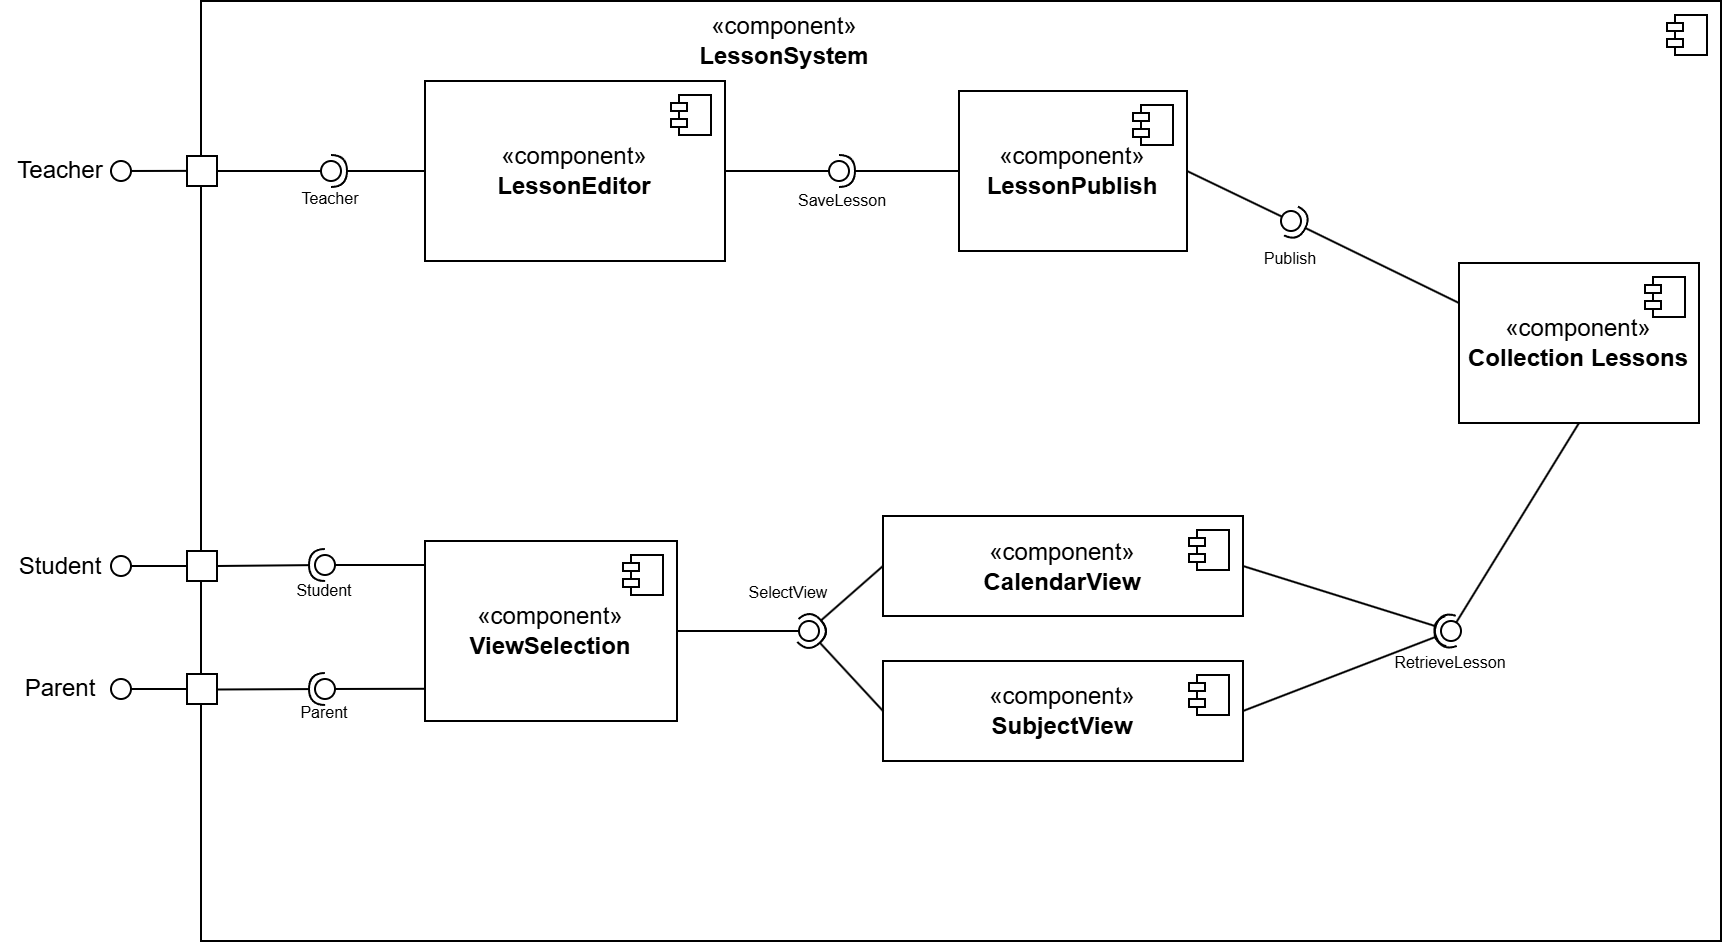
\includegraphics{component-diagram.png}}
	\caption{Komponentní diagram znázorňující tok událostí mezi hlavními částmi systému pro~práci s~výukovými plány.}
	\label{fig:component-diagram}
\end{figure}

Tento komponentní diagram znázorňuje hlavní funkční části systému pro~práci s~výukovými plány a~jejich vzájemné propojení. Učitel využívá \texttt{LessonEditor} výukových plánů k~tvorbě a~úpravě plánů. Po~dokončení může plán uložit, což umožní jeho pozdější úpravy nebo jej pomocí komponenty \texttt{PublishLesson} publikovat. Publikované hodiny se~ukládají do~\texttt{CollectionLessons}, což je hlavní úložiště všech dostupných výukových hodin.

Studenti a~rodiče mají přístup k~výukovým hodinám prostřednictvím komponenty\break\texttt{ViewSelection}, která jim umožňuje volit mezi dvěma režimy zobrazení~--~\texttt{CalendarView} pro~přehledný kalendářní pohled na~hodiny podle data nebo \texttt{SubjectView}, kde jsou hodiny organizovány podle předmětů. Oba způsoby zobrazují relevantní výukové hodiny uložené\break v~\texttt{CollectionLessons}.


\section{Odůvodnění výběru technického zásobníku}

Výběr správného technického zásobníku je zásadním krokem při~návrhu softwaru, který ovlivňuje celý životní cyklus projektu, od~vývoje až po~nasazení a údržbu. Zvolená architektura a~technologie přímo ovlivňují flexibilitu, škálovatelnost, výkon a~také efektivitu práce vývojového týmu. Důležité je zohlednit nejen technické požadavky, ale také zkušenosti týmu a~dostupné zdroje. Tato kapitola se zaměřuje na zdůvodnění volby konkrétního technického zásobníku pro systémy \textit{EDUBO} a~\textit{Eduklub~--~plány výuky}.

\subsection{Výběr architektury}

Při návrhu architektury softwaru byly zvažovány různé přístupy, včetně monolitické a~mikroservisní architektury. Pro~oba projekty, \textit{EDUBO} i~\textit{Eduklub~--~plány výuky}, byla zvolena monolitická architektura ve~spojení s~Docker Compose. Tato volba byla ovlivněna jednoduchostí vývoje, nasazení a~správy systému, což bylo klíčové vzhledem k~velikosti projektů a~zkušenostem týmu.

Monolitická architektura umožnila integrovat všechny části aplikace do~jednoho repozitáře, což zjednodušilo správu kódu i~týmovou spolupráci. Všechny komponenty systému běží společně, což minimalizuje složitost při komunikaci mezi jednotlivými částmi aplikace, jako je frontend, backend a~databáze.

\subsection{Frontend}

Pro~oba projekty \textit{EDUBO} a~\textit{Eduklub~--~plány výuky}, byl jako frontendová technologie zvolen React, což je populární framework pro~tvorbu uživatelských rozhraní. Tento výběr byl založen především na~zkušenostech týmu a~požadavcích na~rychlé a~dynamické uživatelské rozhraní.

React umožňuje vytvářet komponentově orientované aplikace, což znamená, že jednotlivé části uživatelského rozhraní (například tlačítka, formuláře nebo karty) jsou vytvořeny jako samostatné komponenty, které lze znovu použít v~různých částech aplikace. Tato modularita usnadňuje nejen vývoj, ale také údržbu a~rozšiřování systému.

\needspace{9\baselineskip}
Důvody výběru Reactu:
\begin{enumerate}
	\item Zkušenosti týmu: Většina vývojového týmu měla zkušenosti s~Reactem, což umožnilo rychlejší začátek vývoje a~minimalizovalo potřebu doučování se~nových technologií.
	\item Podpora mobilního zobrazení: Ačkoliv byla zvažována alternativa React Native pro~mobilní aplikace, zvolený přístup s~Reactem a~responsivním designem byl dostatečný pro~zajištění kompatibility na~mobilních zařízeních.
	\item Komunitní podpora a~ekosystém: React je široce podporován vývojářskou komunitou, což poskytlo přístup k~rozsáhlé dokumentaci, nástrojům a~knihovnám (např.~React Router, Redux nebo react-beautiful-dnd).
\end{enumerate}

Pro~sestavení frontendového kódu byly použity různé sestavovací nástroje. \textit{EDUBO} bylo původně vytvořeno pomocí Create React App, což je jednoduchý a~dobře známý nástroj pro~rychlé vytvoření React aplikací. Naopak \textit{Eduklub~--~plány výuky} byl vyvíjen s~použitím moderního sestavovacího nástroje Vite, který nabízí rychlejší a~efektivnější vývoj, díky okamžitému znovu načtení modifikací kódu a~optimalizovanému balíčkování.

Během vývoje se~ukázalo, že Vite výrazně urychluje práci s~kódem, což vedlo k~rozhodnutí reinženýrovat \textit{EDUBO} na~stejný sestavovací nástroj. Tato změna se~uskutečnila až ve~fázi údržby, ale přinesla mi rychlejší zpětnou vazbu při~opravách chyb v~aplikaci.

React byl nasazen jako build (sestavená aplikace), který poskytuje optimalizovaný a~produkční kód pro~rychlé načítání aplikace v~prohlížeči. Tento build byl dále servírován pomocí reverzního proxy serveru NGINX, což zajišťovalo rychlou a~bezpečnou distribuci frontendového kódu uživatelům.

\subsection{Backend}

Backendová část aplikací \textit{EDUBO} a~\textit{Eduklub~--~plány výuky} byla navržena s~ohledem na~rozdílné požadavky obou projektů, což vedlo k~použití různých frameworků. Zatímco \textit{EDUBO} bylo vytvořeno pomocí mikro-frameworku Flask, pro~\textit{Eduklub~--~plány výuky} bylo zvoleno robustnější Django. Tento rozdíl reflektuje specifické potřeby každého projektu a~zkušenosti získané během vývoje.

\subsubsection{EDUBO: Flask}

Flask byl vybrán pro~\textit{EDUBO} především díky své jednoduchosti, rychlému nastavení a~zkušenostem týmu. Flask je mikro-framework v~Pythonu, který umožňuje vývojářům flexibilně přizpůsobit architekturu projektu jejich potřebám.

\needspace{7\baselineskip}
Mezi klíčové výhody Flasku patří:
\begin{itemize}
	\item \textbf{Flexibilita:} Flask poskytuje svobodu v~návrhu projektu, protože nevyžaduje pevnou strukturu.
	\item \textbf{Nízká složitost:} Ideální pro~menší aplikace nebo prototypy, kde není potřeba složitá logika nebo vestavěné funkce.
	\item \textbf{Kompatibilita s~rozšířeními:} Umožňuje snadno integrovat nástroje a~knihovny třetích stran podle aktuálních potřeb projektu.
\end{itemize}

\needspace{7\baselineskip}
Nicméně během vývoje se objevily i~významné nevýhody:
\begin{itemize}
	\item \textbf{Chybějící migrace:} Nutnost manuálních úprav databázové struktury zpomalovala vývoj a~zvyšovala pravděpodobnost chyb.
	\item \textbf{Základní správa uživatelů:} Omezené možnosti nativní autentizace a~správy uživatelských práv si vyžádaly dodatečnou práci.
	\item \textbf{Absence jasné struktury:} Flexibilita může být nevýhodou u~větších projektů, kde chybí standardizovaný přístup k~organizaci kódu.
\end{itemize}

Flask byl vhodnou volbou pro~rychlý začátek vývoje, avšak při nárůstu komplexity projektu se ukázalo, že by robustnější framework zjednodušil dlouhodobou údržbu.

\subsubsection{Eduklub~--~plány výuky: Django}

Pro~\textit{Eduklub~--~plány výuky} bylo zvoleno Django, což je plnohodnotný framework v~Pythonu, který nabízí rozsáhlé vestavěné funkce a~jasnou strukturu. Django se osvědčilo zejména u~projektů, které vyžadují vyšší míru komplexnosti a~robustní řešení.

\needspace{7\baselineskip}
Mezi klíčové výhody Djanga patří:
\begin{itemize}
	\item \textbf{Komplexní nástroje:} Vestavěná podpora pro~migrace, autentizace, správu uživatelských práv a~ORM výrazně zjednodušila vývoj.
	\item \textbf{Standardizace:} Jasná a~přehledná struktura projektu usnadnila spolupráci v~týmu a~přehlednost kódu.
	\item \textbf{Rychlost vývoje:} Vestavěné administrativní rozhraní a~šablonovací systém umožnily rychlé nasazení nových funkcí.
\end{itemize}

\needspace{7\baselineskip}
Na~druhou stranu, Django má i~své nevýhody:
\begin{itemize}
	\item \textbf{Nižší flexibilita:} Pevně daná struktura a~pravidla mohou být omezením pro~projekty s~netypickými požadavky.
	\item \textbf{Komplexnost:} U~menších projektů může být Django zbytečně složité, což může zpomalit vývoj při nízkých nárocích.
	\item \textbf{Vyšší počáteční nároky:} Vzhledem k~většímu množství funkcí a~možností vyžaduje Django delší dobu na~naučení a~nastavení.
\end{itemize}

Django bylo jasnou volbou pro~tuto platformu, díky své schopnosti efektivně řešit komplexní potřeby projektu, což by s~Flaskem nebylo možné bez výrazně vyššího úsilí.

\newpage

\subsubsection{Srovnání Flasku a Djanga}

Zatímco Flask je ideální pro~menší aplikace, kde je potřeba rychle začít vývoj a~přizpůsobit strukturu projektu, Django vyniká u~větších projektů svou robustností a~bohatou sadou vestavěných nástrojů. Obě technologie přinášejí výhody v~závislosti na~konkrétních požadavcích projektu a~zkušenostech vývojového týmu.

Oba backendy byly nasazeny jako samostatné služby v~kontejnerech pomocí Dockeru. Tyto kontejnery byly spravovány pomocí Docker Compose, což umožnilo snadnou integraci s~dalšími částmi systému, jako je databáze a~frontend.

\subsection{Databáze}

Pro databázovou vrstvu byly v~projektech \textit{EDUBO} a~\textit{Eduklub~--~plány výuky} použity různé přístupy reflektující jejich specifické požadavky a~potřeby. V~systému \textit{EDUBO} byla zvolena MongoDB, zatímco ve~webovém agregátoru byla použita relační databáze PostgreSQL.

\subsubsection{EDUBO: MongoDB}

MongoDB byla původně vybrána díky své flexibilitě při ukládání nestrukturovaných dat. Její schopnost pracovat s~dokumenty ve~formátu JSON, které jsou interně ukládány ve~formátu BSON (binární JSON), umožnila snadné ukládání nestrukturovaných dat z~frontendu a~efektivnější práci s~daty díky optimalizovanému ukládání a~rychlému přístupu.

\needspace{4\baselineskip}
Hlavní výhody MongoDB zahrnují:
\begin{itemize}
	\item \textbf{Flexibilní datový model:} Umožnil snadné ukládání různorodých dat bez nutnosti předem definovaných schémat.
	\item \textbf{Škálovatelnost:} MongoDB nabízí jednoduché horizontální škálování.
\end{itemize}

\needspace{5\baselineskip}
Nicméně během vývoje se ukázaly i~významné nevýhody:
\begin{itemize}
	\item \textbf{Chybějící relace:} Komplikovalo to práci s~datovými vazbami, což vedlo k~potřebě složitějších dotazů a~manuálního zpracování referencí.
	\item \textbf{Manuální úpravy struktury:} Kvůli absenci migrací bylo nutné měnit databázovou strukturu ručně při každé aktualizaci, což zvyšovalo riziko chyb.
\end{itemize}

\subsubsection{Eduklub~--~plány výuky: PostgreSQL}

Pro \textit{Eduklub~--~plány výuky} byla zvolena PostgreSQL relační databáze, která lépe odpovídala potřebám rozsáhlejší aplikace a~zjednodušila práci s~datovými vztahy.

\needspace{7\baselineskip}
Mezi její hlavní výhody patří:
\begin{itemize}
	\item \textbf{Podpora relací:} Relace mezi tabulkami umožnily efektivní a~přehledné ukládání datových vazeb.
	\item \textbf{Stabilita a výkon:} PostgreSQL je známá svou spolehlivostí a~schopností pracovat s~velkými objemy dat.
	\item \textbf{Vestavěná podpora pro migrace:} Díky integraci s~Djangem byla práce s~databází výrazně efektivnější.
\end{itemize}

\subsection{NGINX a Docker}

Pro správu a~nasazení obou systémů byly využity nástroje NGINX jako reverzní proxy server a~Docker pro kontejnerizaci všech aplikací a~jejich komponent.

\subsubsection{NGINX}

NGINX byl použit k~optimalizaci síťové komunikace mezi frontendem, backendem a~uživateli.

\needspace{8\baselineskip}
Hlavní úloha NGINX spočívala~v:
\begin{itemize}
	\item \textbf{Směrování požadavků:} NGINX přesměrovává API požadavky na~backend a~ostatní požadavky na~frontend, čímž zajišťuje efektivní distribuci zatížení.
	\item \textbf{Bezpečnostní filtrování:} Chrání aplikace před nežádoucími požadavky a~útoky.
	\item \textbf{Zrychlení načítání dat:} Ve fázi údržby byl přidán kompresní nástroj Brotli, který umožnil odesílání statických souborů (např.~JavaScript, CSS nebo obrázky) v~co nejmenší velikosti. Statické soubory byly předem komprimovány na~nejvyšší možnou úroveň, což výrazně snížilo množství přenášených dat a~zlepšilo uživatelský zážitek díky rychlejšímu načítání.
\end{itemize}

\subsubsection{Docker}

Docker je klíčovým nástrojem pro kontejnerizaci všech komponent aplikace, včetně frontendu, backendu, databáze a~NGINX.

\needspace{7\baselineskip}
Hlavní přínosy Dockeru zahrnují:
\begin{itemize}
	\item \textbf{Izolace prostředí:} Každá část aplikace běží v~odděleném kontejneru, což eliminuje konflikty závislostí mezi různými komponentami.
	\item \textbf{Snadné nasazení:} Docker Compose umožňuje definovat konfiguraci všech kontejnerů v~jednom souboru, což zjednodušilo jejich spuštění na~různých prostředích.
	\item \textbf{Přenositelnost:} Docker zajistil, že aplikace může být spuštěna na~libovolném serveru s~minimální konfigurací.
\end{itemize}

Technický zásobník použitý v~aplikacích \textit{EDUBO} a~\textit{Eduklub~--~plány výuky} byl vybrán s~ohledem na~specifické požadavky obou projektů, zkušenosti týmu a~potřebu efektivního vývoje. Monolitická architektura a~kontejnerizace pomocí Dockeru zajistily jednoduché nasazení a~správu aplikací, zatímco React pro~frontend poskytl moderní a~dynamické uživatelské rozhraní. Ačkoliv původní volba Flasku a~MongoDB pro~\textit{EDUBO} nebyla ideální a~přinesla komplikace spojené s~absencí robustních nástrojů a~relací, zkušenosti získané během vývoje vedly k~použití Django a~PostgreSQL v~\textit{Eduklub~--~plány výuky}, což se ukázalo jako efektivnější řešení pro~komplexnější aplikace.


\section{Implementace softwaru pro plánování výuky}

Během vývoje \textit{EDUBO} bylo nutné navrhnout a~implementovat robustní systém pro tvorbu a~organizaci výukových plánů. Celý proces byl rozdělen do~dvou iterací, přičemž každá z~nich se zaměřovala na~konkrétní funkcionalitu systému. Mezi hlavní cíle patřilo vytvoření editoru výukových plánů, který umožní učitelům intuitivně sestavovat své plány, dále vyvinout systém pro publikaci výukových hodin, díky kterému budou mít studenti snadný přístup ke~svým rozvrhům a~možnosti exportu výukových plánů do~PDF. Vývoj probíhal ve~spolupráci se~společnostmi DataPLEX~Consulting,~s.r.o. a~Databig~s.r.o., které poskytly odborné konzultace a~zpětnou vazbu k~implementovaným řešením.

\subsection{Vývojový proces a~týmová spolupráce}

V~první iteraci byl vytvořen editor výukových plánů, který poskytuje učitelům nástroje pro snadné sestavování výukových plánů. Druhá iterace se soustředila na~zpřístupnění hodin studentům, což zahrnovalo jejich publikaci a~správu v~uživatelském rozhraní.

Na~vývoji se podílel tým studentů Univerzity~Jana~Evangelisty~Purkyně a~Gymnázia~Josefa~Jungmanna~v~Litoměřicích, přičemž role jednotlivých členů se postupně měnily podle aktuálních potřeb projektu. Projekt byl řízen agilní metodikou Scrum, která umožnila iterativní vývoj, pravidelné testování a~rychlou reakci na~zpětnou vazbu.

\begin{itemize}
	\item \textbf{Pavel Beránek} byl projektovým manažerem v~první iteraci a~zajišťoval řízení projektu, komunikaci se~stakeholdery a~organizaci vývojových aktivit. Ve~druhé iteraci tuto roli převzal \textbf{Lukáš Polidar}.
	\item \textbf{Matěj Kaška (já)} byl hlavním backend programátorem v~první iteraci a~od~druhé iterace převzal i~roli hlavního programátora a~Scrum mastera, zajišťujícího vedení týmu a~organizaci sprintů.
	\item Na~frontendu pracoval v~první iteraci \textbf{Jan Plechatý}, který byl hlavním frontend programátorem. Spolu s~ním se~na~vývoji podíleli \textbf{Vojtěch Kunc} a~\textbf{Vlasta Michalcová}, která byla součástí týmu během všech tří iterací. Od~druhé iterace převzal roli hlavního frontend programátora \textbf{Lukáš Priban}.
	\item \textbf{Andrej Dunda} a~\textbf{Tomáš Svoboda} působili jako juniorní programátoři, přičemž Andrej Dunda se zaměřoval na~frontend a~Tomáš Svoboda měl na~starosti testování a~vývoj backendu i~frontendu.
	\item Návrh uživatelského rozhraní a~UX designu v~prvních dvou iteracích měla na~starosti \textbf{Kateřina Pazderová}.
	\item Na~backendu pracoval kromě mě také \textbf{Lukáš Jurásek}, kterého ve~druhé iteraci nahradil \textbf{Jakub Kopecký} jako hlavní backend programátor.
\end{itemize}

Komunikace v~týmu probíhala prostřednictvím Discordu, kde se konaly pravidelné stand-up meetingy, během nichž se hodnotil pokrok a~plánovala se následující iterace. Pro řízení úkolů byla využívána Kanban tabule v~ClickUpu, což umožňovalo efektivní organizaci práce.

Pro verzování kódu byl využíván software Git ve~spojení s~GitHubem, kde jsme dodržovali standardizované pojmenovávání větví a~workflow zahrnující pull requesty a~issues. Každá nová funkcionalita byla vyvíjena v~samostatné větvi (např.~\texttt{feature/xxx}, \texttt{fix/xxx}), která byla následně schválena pomocí code review před sloučením do~hlavní vývojové větve.

\subsection{Návrh uživatelského rozhraní ve~Figma}

Vývoj uživatelského rozhraní aplikace začal ručně kresleným wireframem (drátěný model), který vytvořili pedagogové Univerzity Karlovy. Tento návrh na~papíře sloužil jako prvotní koncept aplikace, ve~kterém se objevily základní požadavky na~funkčnost editoru výukových plánů. I~když měl tento návrh jasně definovanou strukturu, většina komponent byla v~průběhu dalšího vývoje odstraněna nebo přeuspořádána. Zachovalo se však základní rozvržení plátna.

\begin{figure}[H]
	\centering
	\resizebox{12cm}{!}{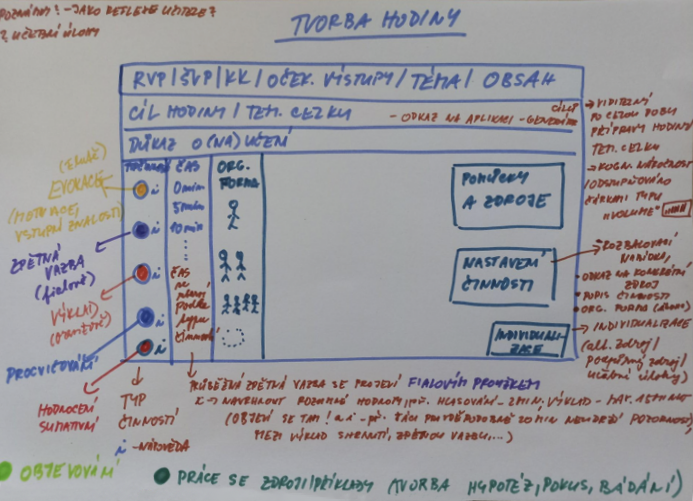
\includegraphics{edubo-navrh-1.png}}
	\caption{Prvotní ručně kreslený návrh uživatelského rozhraní editoru aplikace \textit{EDUBO}.}
	\label{fig:edubo-navrh-1}
\end{figure}

Na~základě tohoto návrhu vznikla první digitální verze v~aplikaci Figma, kterou vytvořila \textbf{Kateřina Pazderová}. Tento návrh se již více podobal finálnímu vzhledu aplikace, ale stále zde chyběla definitivní vizuální identita~--~například nebyla určena primární barva uživatelského rozhraní. V~tomto návrhu měly typy aktivit kruhový design a~zahrnoval několik funkcí, které nakonec nebyly součástí editoru, ale některé z~nich našly své uplatnění v~jiných částech aplikace. Mezi tyto komponenty patřilo například vyhledávání, přidělování hodin, historie použití a~funkce pro kontrolu plánu a~typ plánu.

\begin{figure}[H]
	\centering
	\resizebox{16cm}{!}{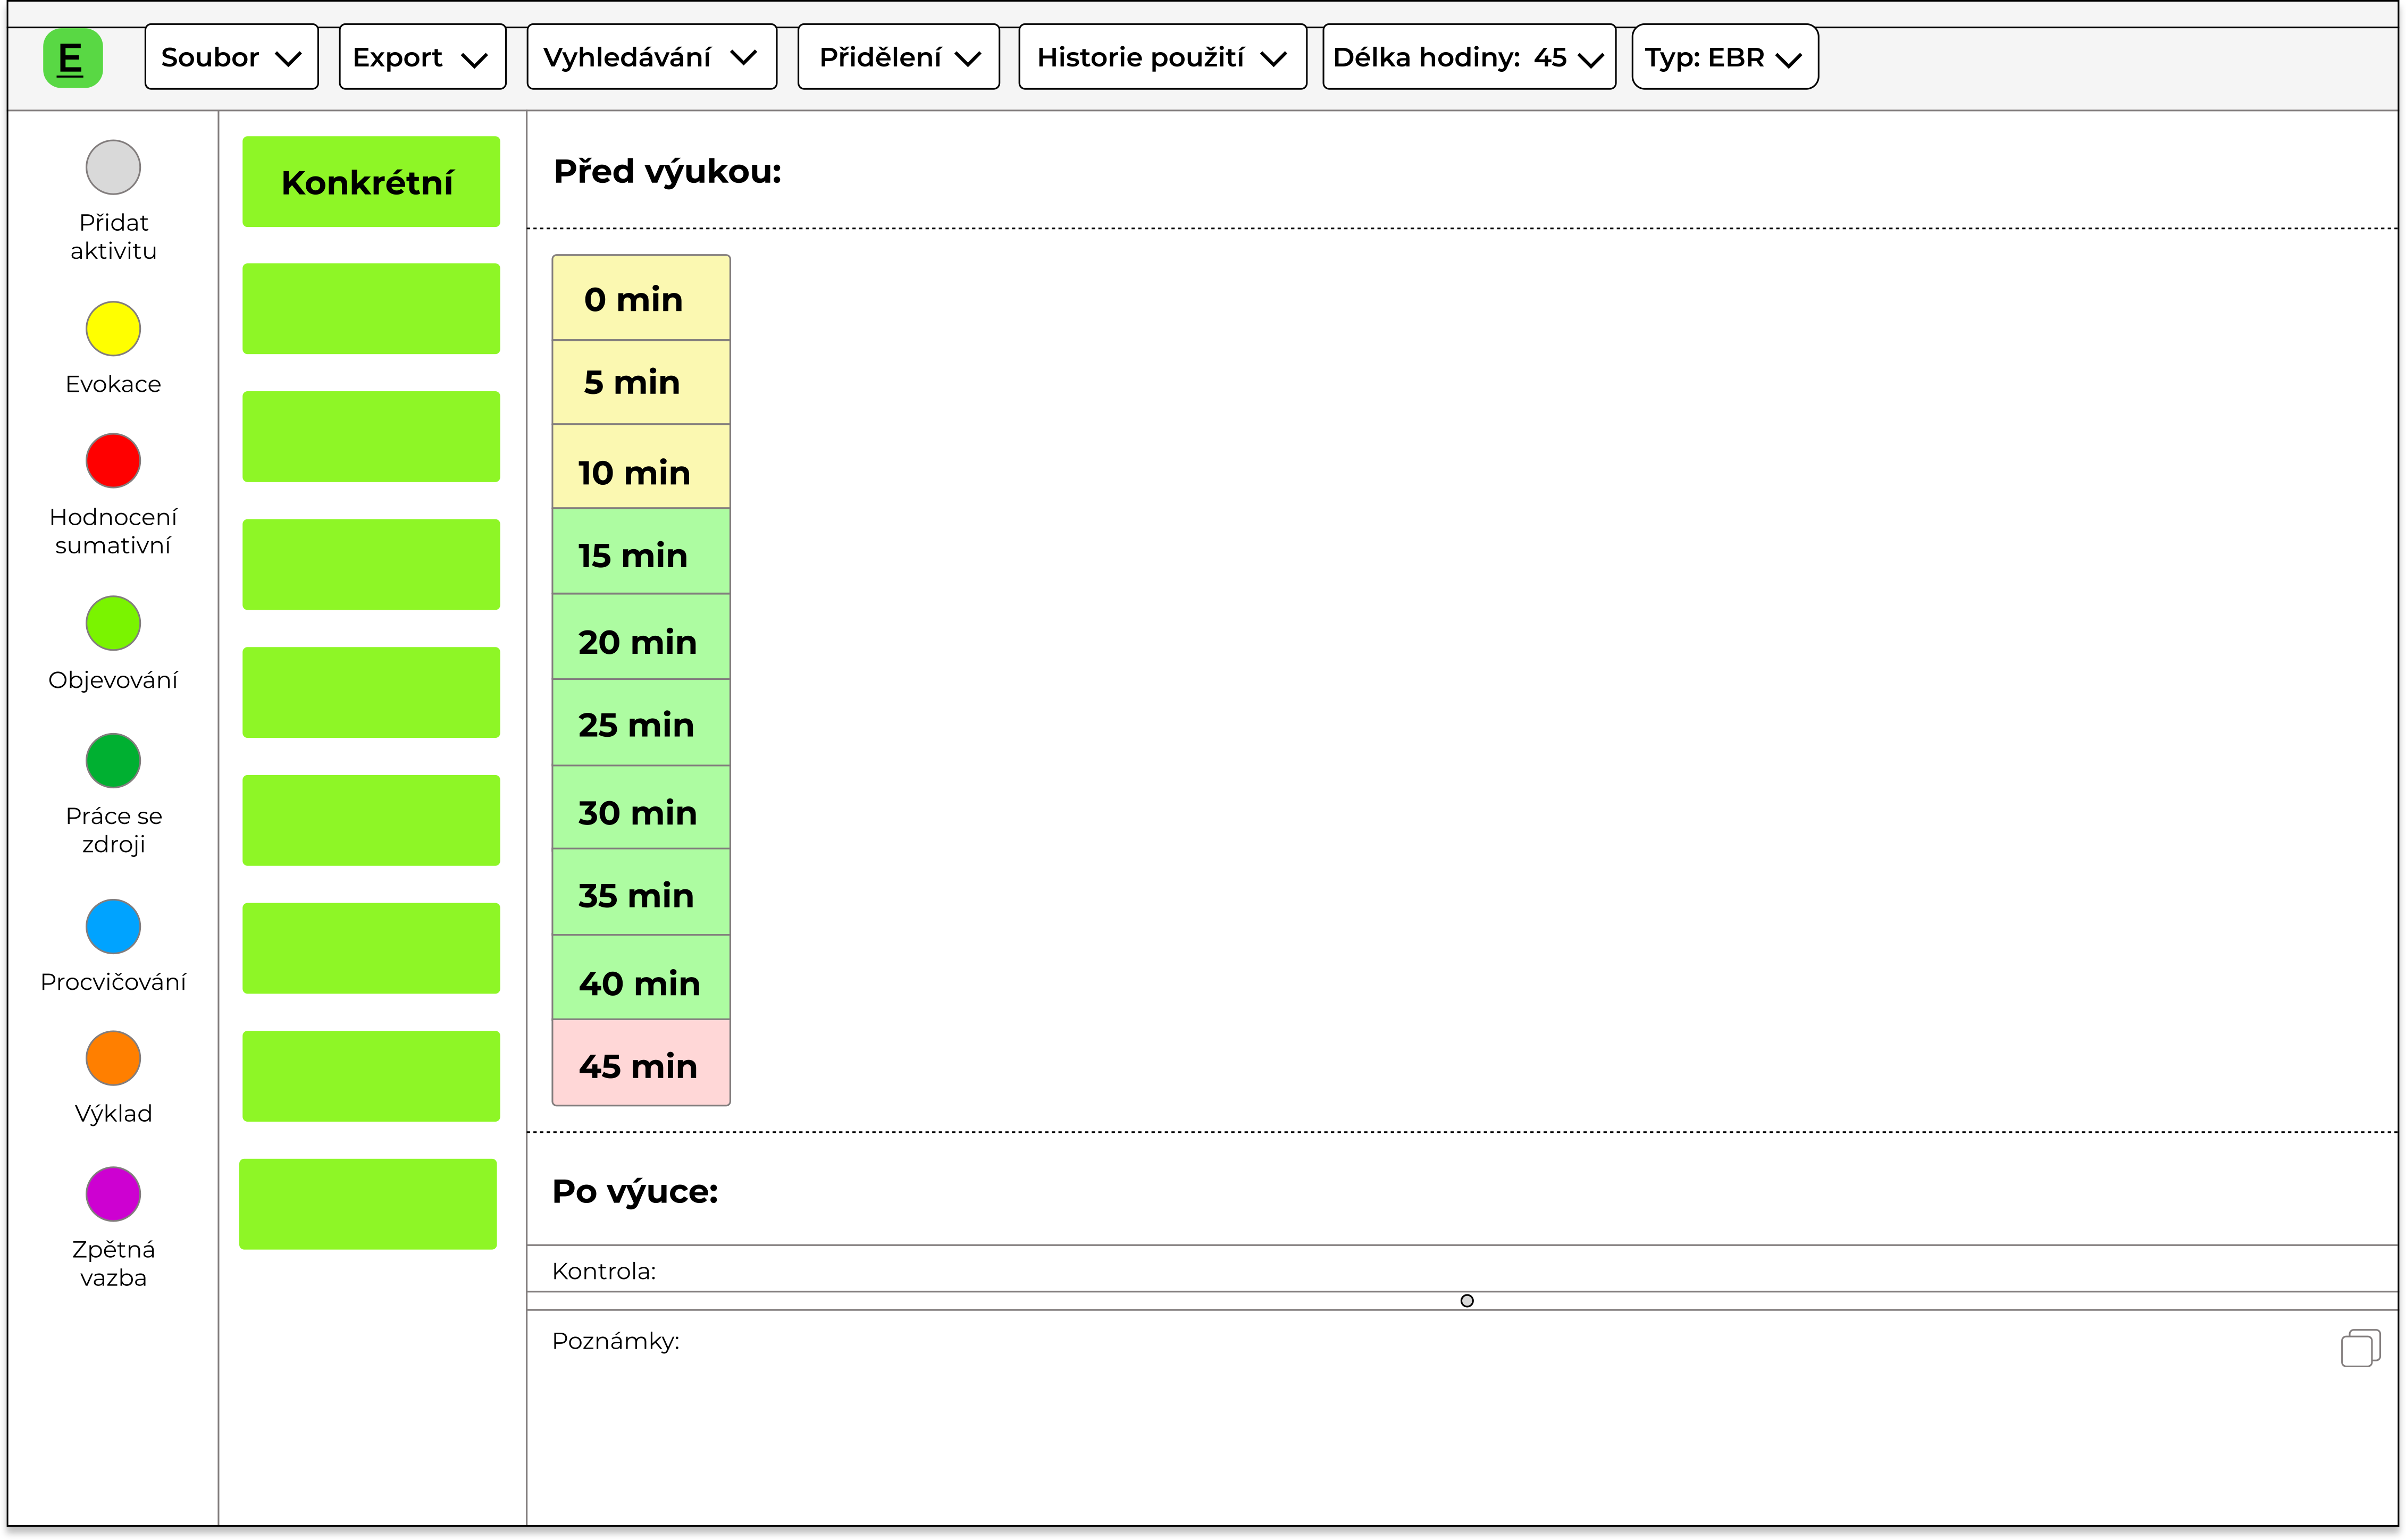
\includegraphics{edubo-navrh-2.png}}
	\caption{Druhý návrh uživatelského rozhraní editoru aplikace \textit{EDUBO}.}
	\label{fig:edubo-navrh-2}
\end{figure}

Třetí návrh v~aplikaci Figma již téměř odpovídal finální podobě aplikace. V~této fázi byla určena hlavní barva uživatelského rozhraní a~vznikl přesný návrh plátna editoru. Tento návrh sloužil jako základ pro implementaci grafického rozhraní v~samotné aplikaci.

\begin{figure}[H]
	\centering
	\resizebox{16cm}{!}{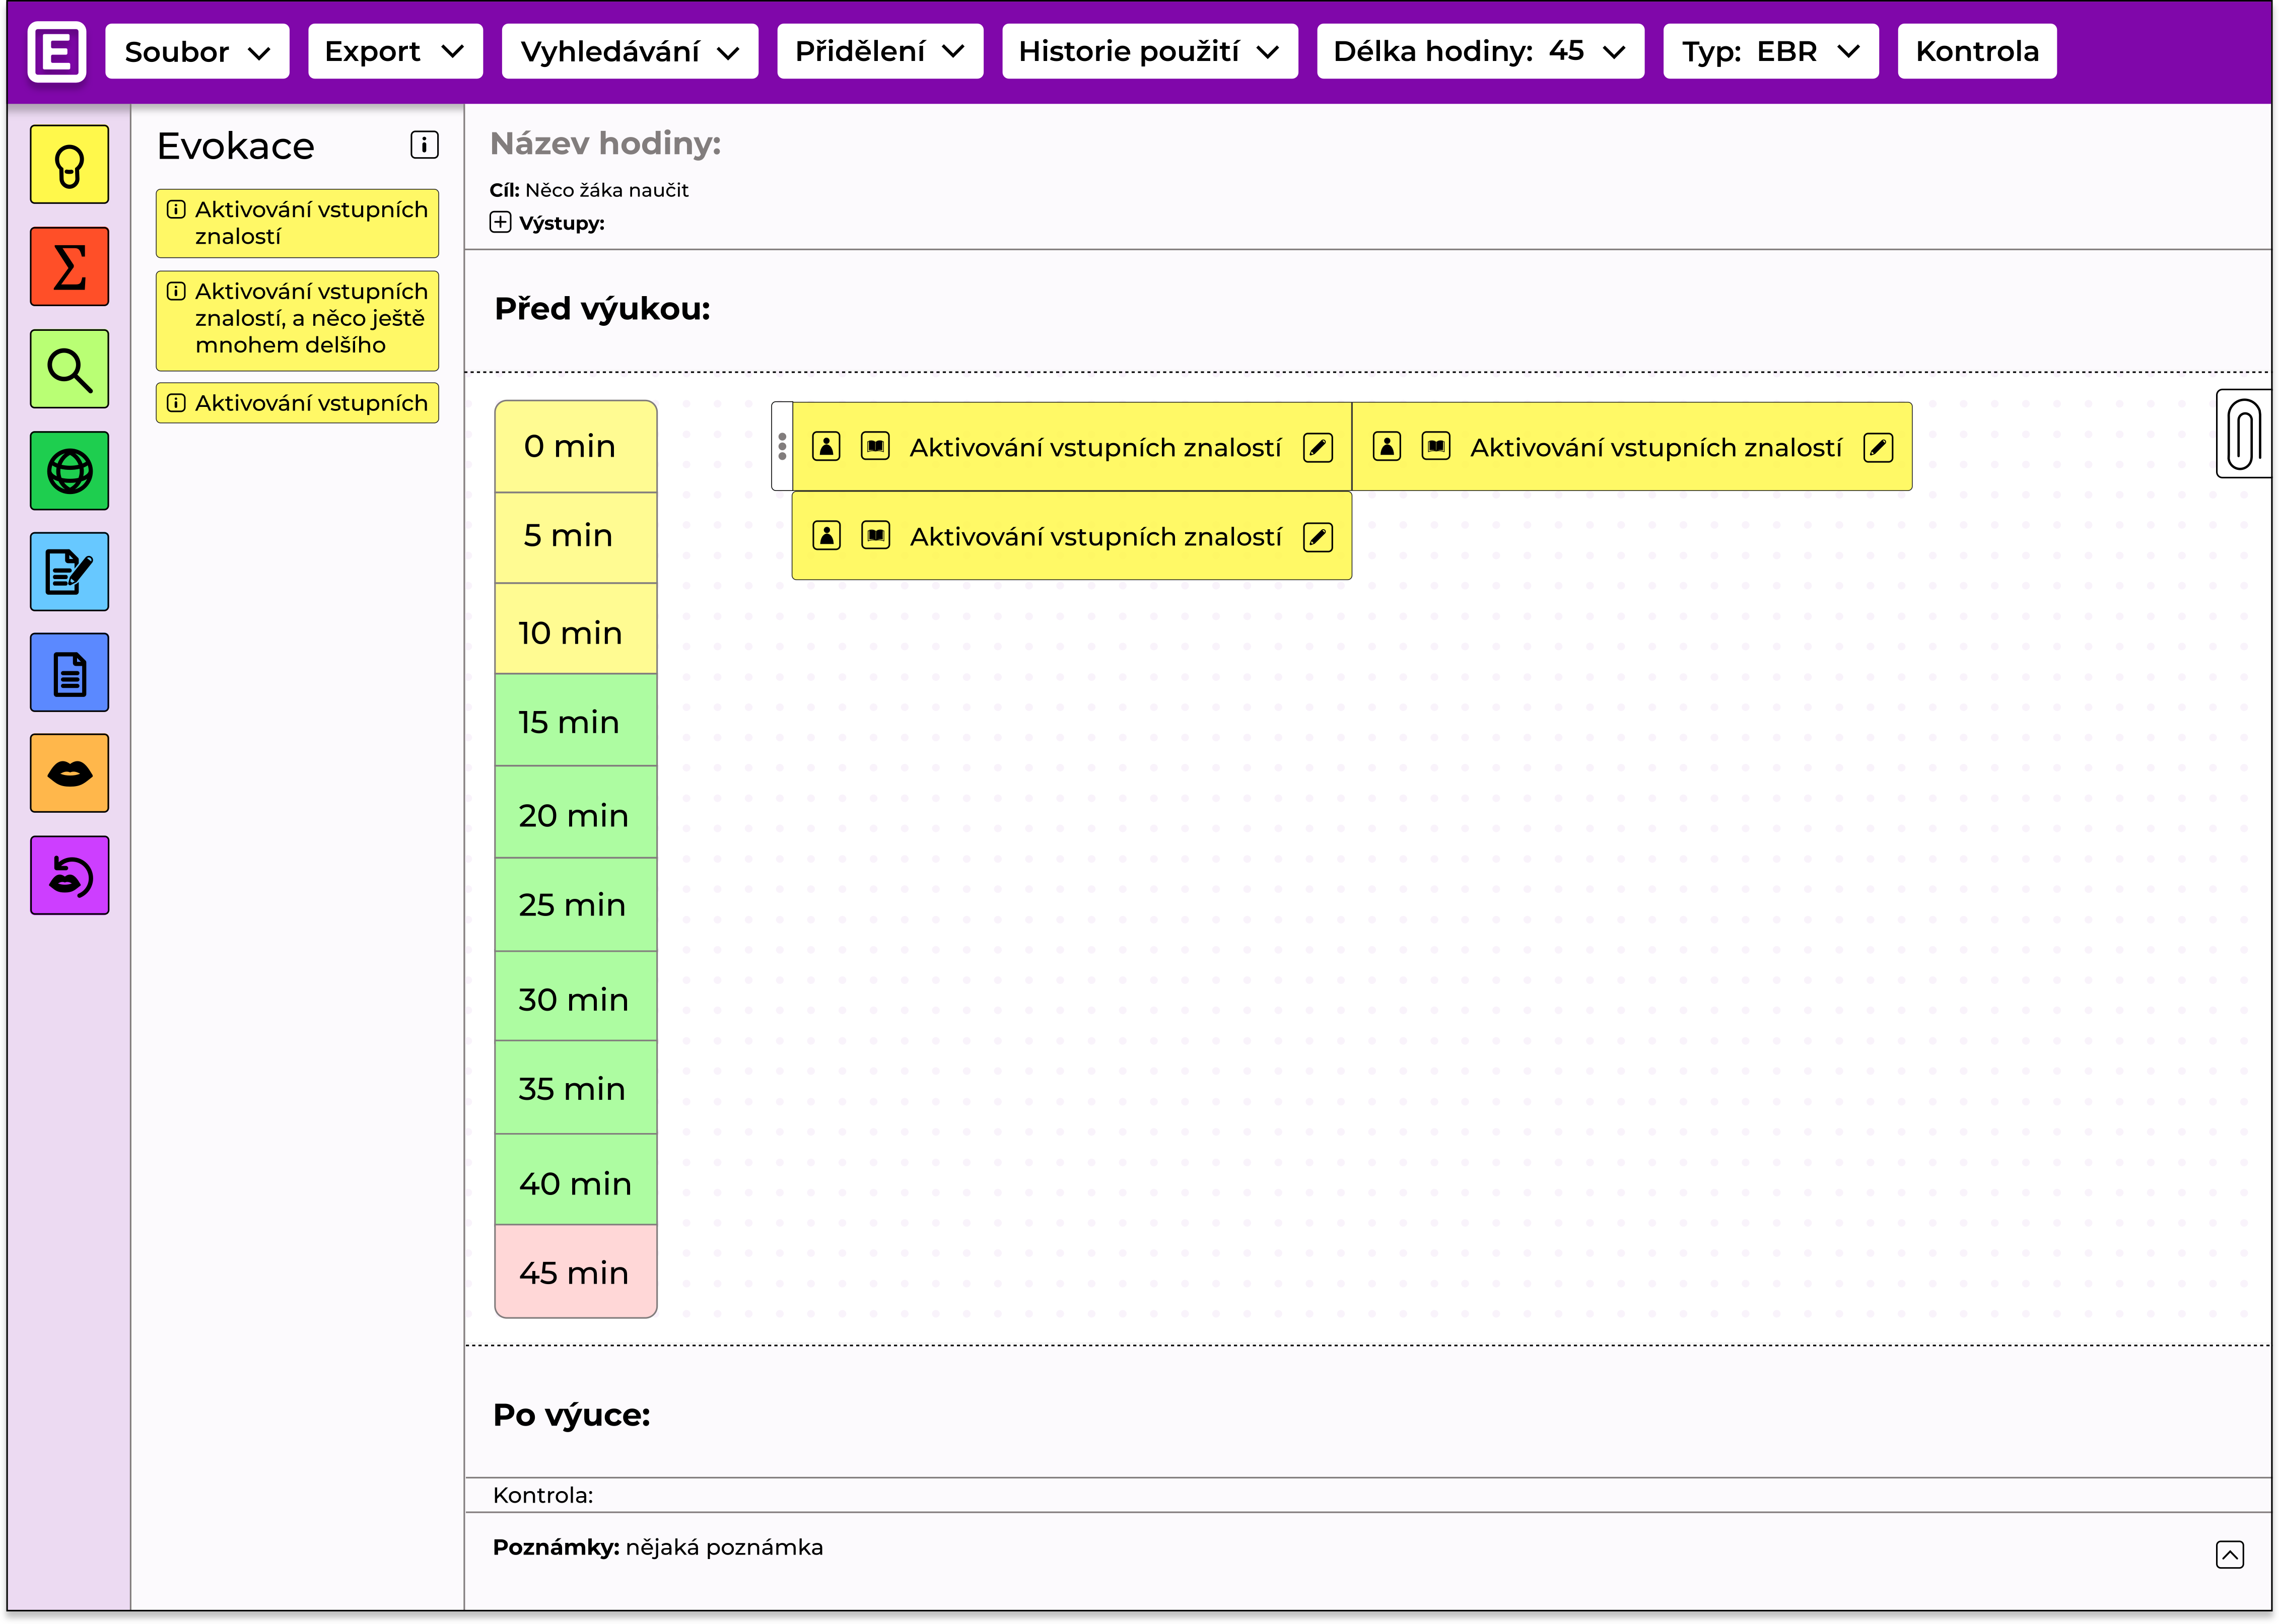
\includegraphics{edubo-navrh-3.png}}
	\caption{Finální návrh uživatelského rozhraní editoru aplikace \textit{EDUBO}.}
	\label{fig:edubo-navrh-3}
\end{figure}

\subsection{Modelování případů užití a procesů}

\begin{figure}[H]
	\centering
	\resizebox{14cm}{!}{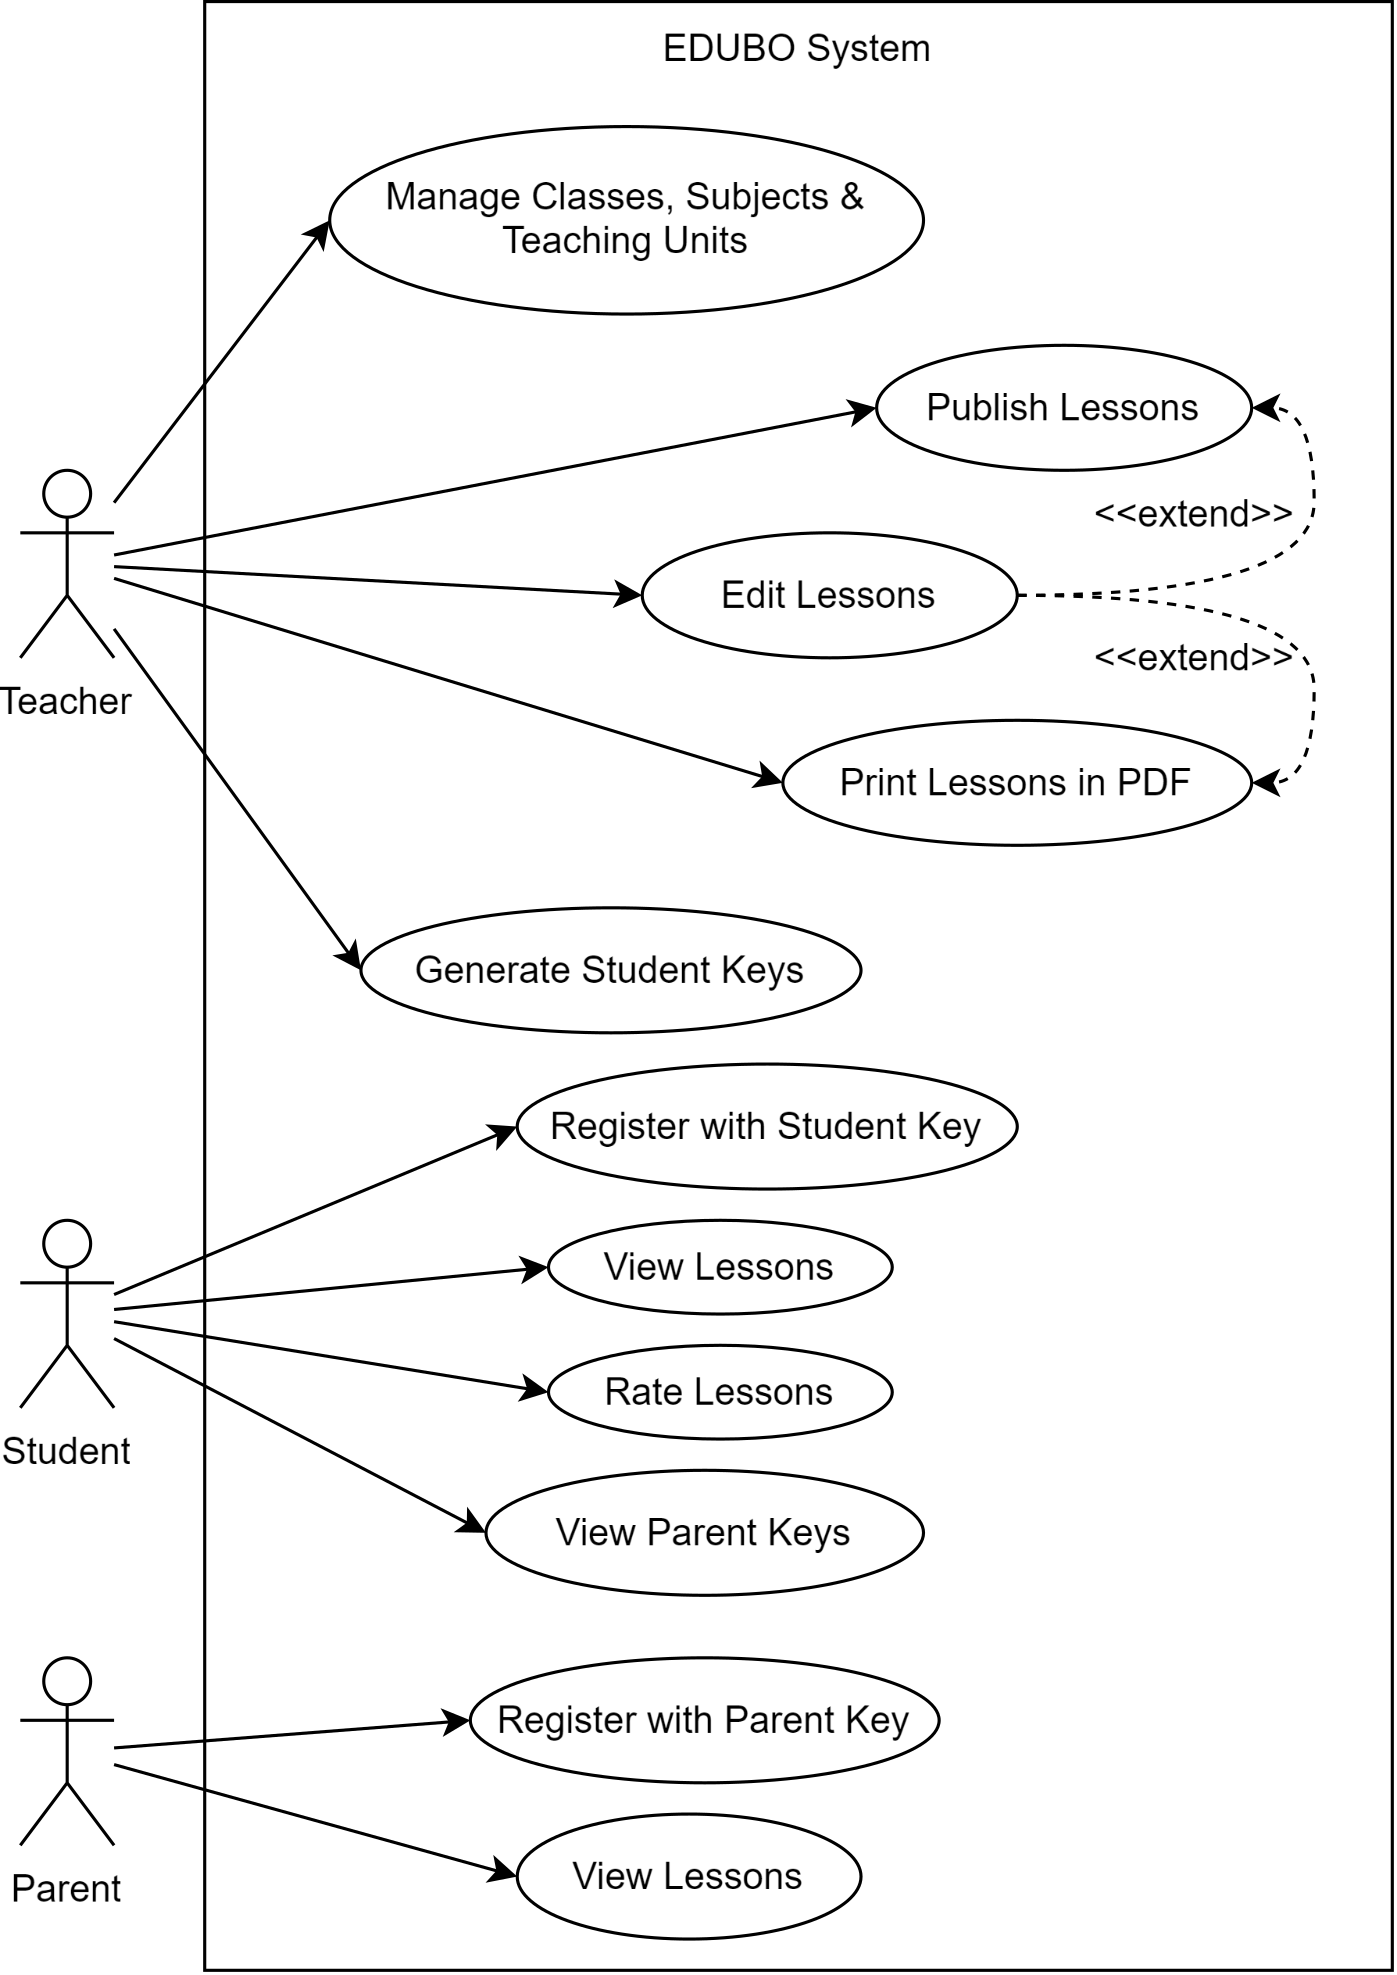
\includegraphics{use-case-diagram.png}}
	\caption{Diagram případů užití ilustrující základní scénáře interakce uživatelů se~systémem.}
	\label{fig:use-case-diagram}
\end{figure}

Tento \textit{use case diagram} popisuje hlavní případy užití (\textit{use cases}) pro tři různé typy uživatelů systému: učitele, studenta a~rodiče. Diagram zobrazuje hlavní způsoby, jak bude systém využíván uživateli. Tyto případy zahrnují správu tříd, výukových jednotek, registraci uživatelů pomocí klíčů a~možnost hodnocení hodin.

\textbf{Teacher (Učitel):}
\begin{itemize}
	\item \textbf{Manage Classes, Subjects \& Teaching Units}:~Učitel může spravovat třídy, předměty a~výukové jednotky v~systému.
	\item \textbf{Edit Lessons}:~Učitel má možnost upravovat hodiny. Tento případ užití je propojen s~dalšími dvěma funkcemi:
	\begin{itemize}
		\item \textbf{Publish Lessons}:~Učitel může publikovat hodiny jako volitelné rozšíření úprav hodin.
		\item \textbf{Print Lessons in PDF}:~Učitel má možnost vytisknout hodiny ve~formátu PDF jako volitelné rozšíření úprav hodin.
	\end{itemize}
	\item \textbf{Generate Student Keys}:~Učitel může generovat registrační klíče pro studenty, které umožňují studentům přihlášení do systému.
\end{itemize}

\vspace{1em}
\textbf{Student (Student):}
\begin{itemize}
	\item \textbf{Register with Student Key}:~Student se může zaregistrovat do systému pomocí registračního klíče, který obdrží od učitele.
	\item \textbf{View Lessons}:~Student má přístup k~prohlížení publikovaných hodin.
	\item \textbf{Rate Lessons}:~Student může hodnotit hodiny.
	\item \textbf{View Parent Keys}:~Student může získat klíče pro rodiče, což jim umožní přístup k~zobrazení hodin.
\end{itemize}

\vspace{1em}
\textbf{Parent (Rodič):}
\begin{itemize}
	\item \textbf{Register with Parent Key}:~Rodič se může zaregistrovat do systému pomocí klíče, který obdržel od studenta.
	\item \textbf{View Lessons}:~Rodič může zobrazit publikované hodiny, které byly přiřazeny jejich studentovi, což jim umožňuje sledovat průběh výuky.
\end{itemize}

\begin{figure}[H]
	\centering
	\resizebox{11cm}{!}{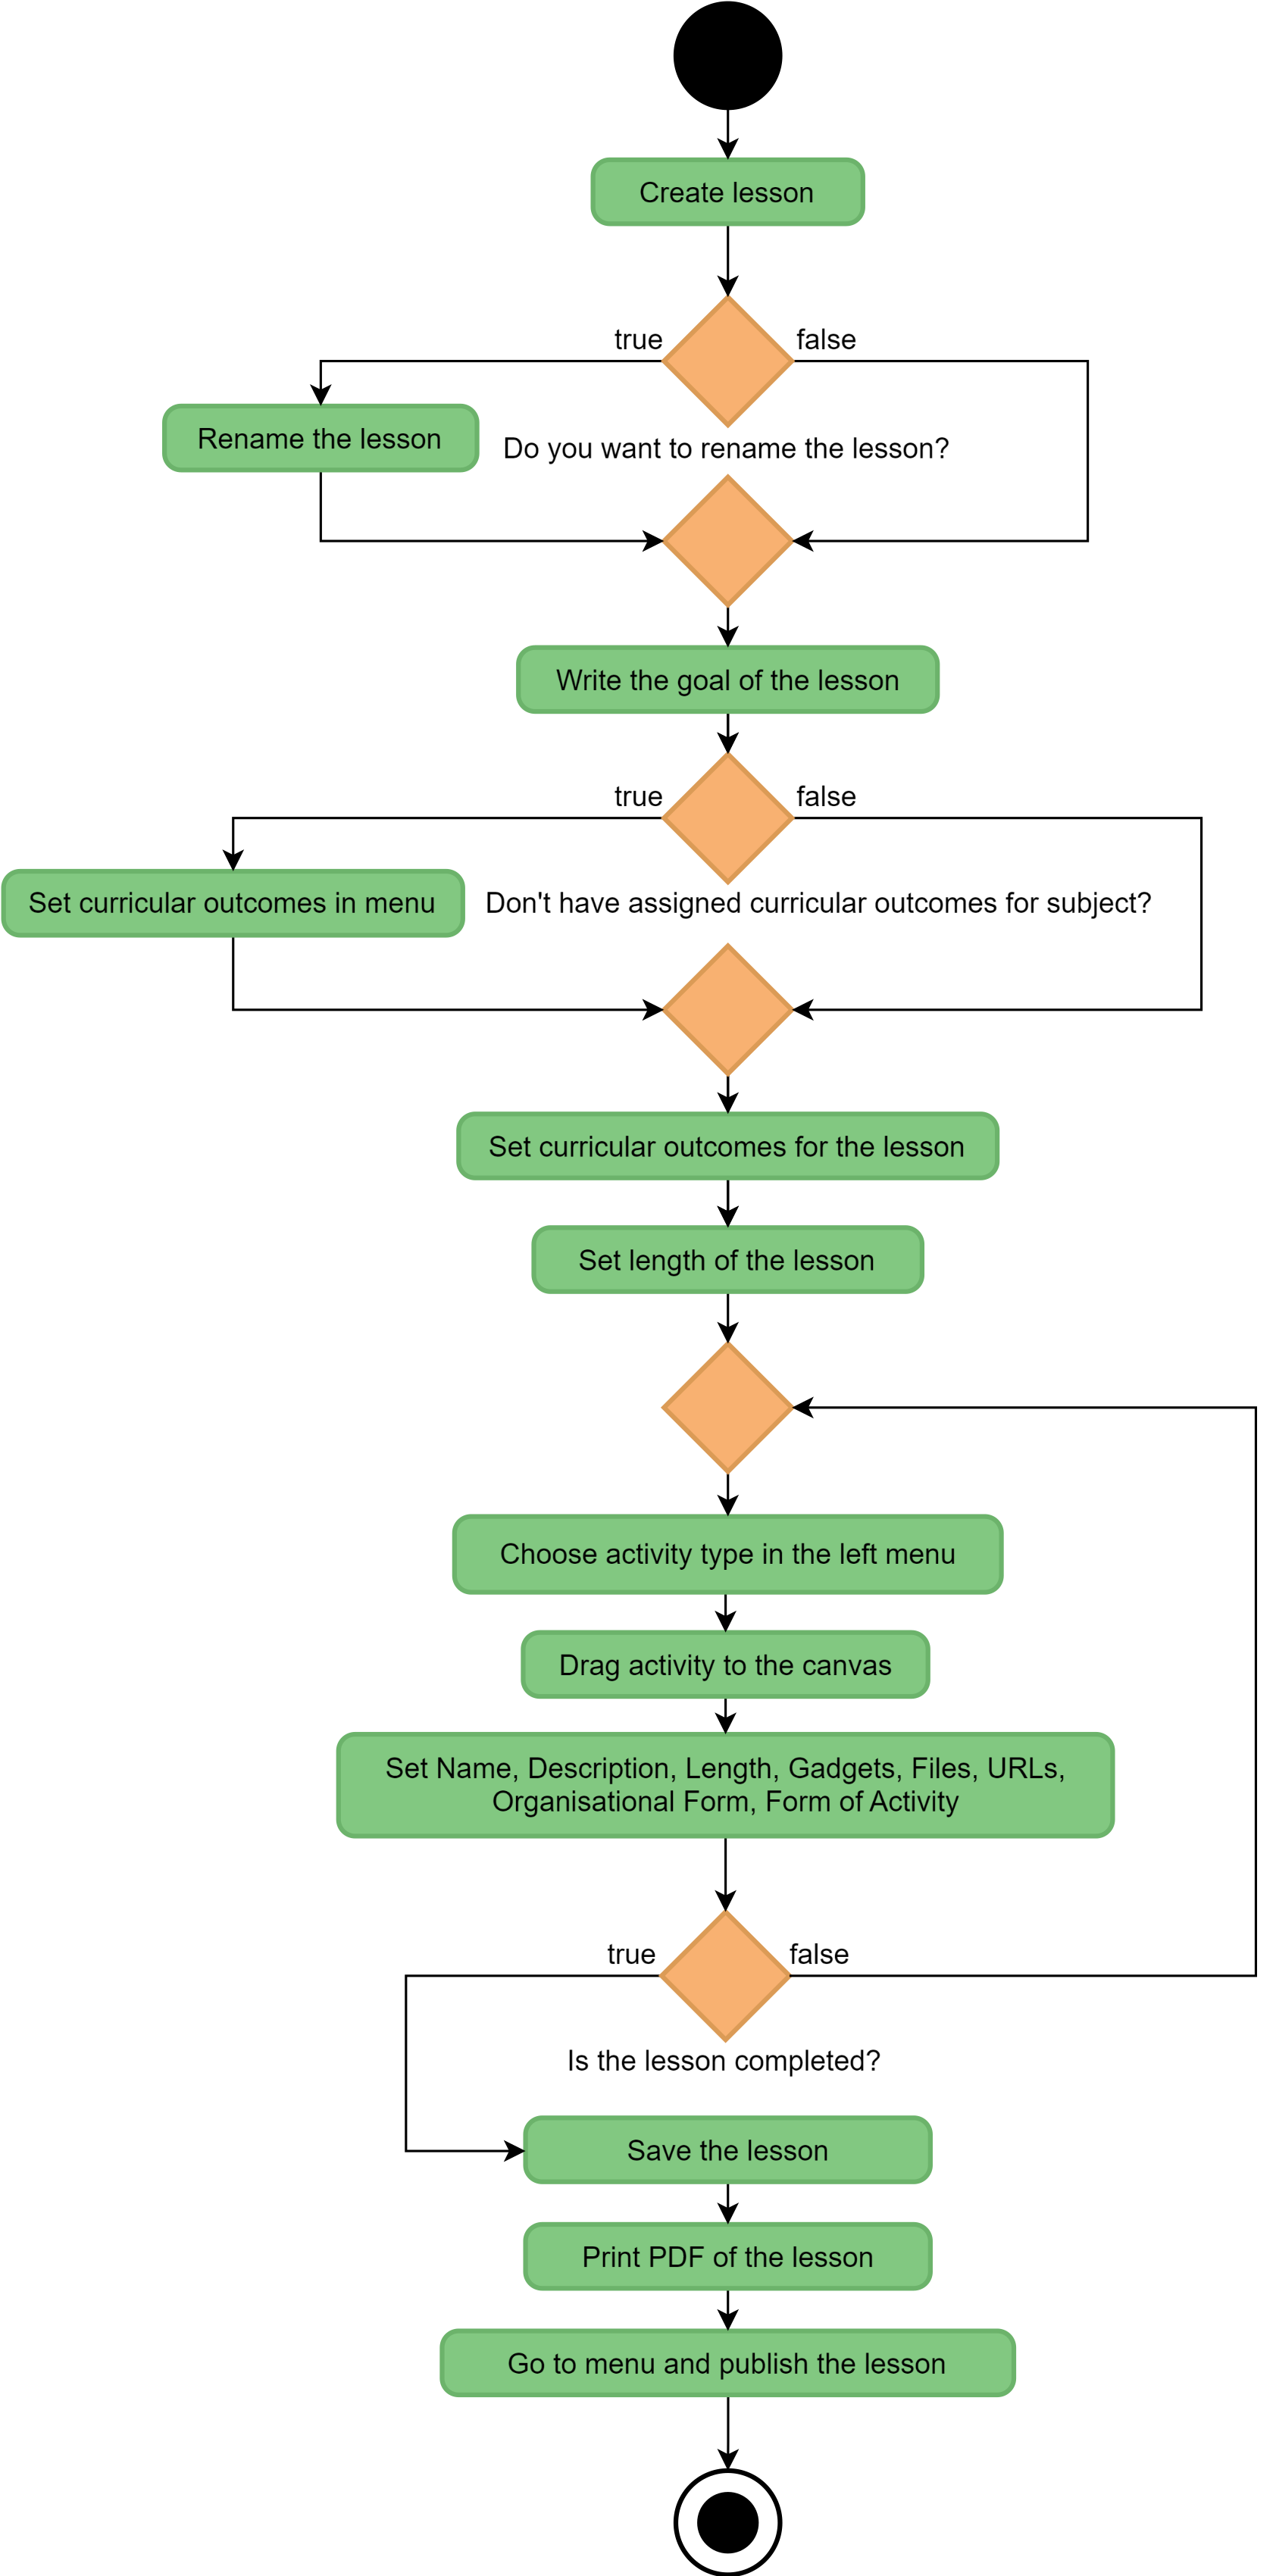
\includegraphics{activity-diagram.png}}
	\caption{Diagram aktivit znázorňující postup při~tvorbě a~publikaci výukového plánu v~aplikaci \textit{EDUBO}.}
	\label{fig:activity-diagram}
\end{figure}

\newpage

Tento diagram aktivit ilustruje proces tvorby hodiny v~aplikaci \textit{EDUBO}. Diagram zobrazuje jednotlivé kroky od vytvoření hodiny až po publikaci hodiny pro studenty. Proces zahrnuje nastavení základních parametrů hodiny, přidání aktivit a~úpravy jejich detailů, a~nakonec uložení a~publikaci vytvořené hodiny.

\begin{enumerate}
	\item \textbf{Vytvoření hodiny:}
	\begin{itemize}
		\item Proces začíná akcí \textit{Create lesson}, kdy uživatel vytvoří výukovou hodinu v~menu.
	\end{itemize}
	
	\item \textbf{Nastavení základních informací o~hodině:}
	\begin{itemize}
		\item Uživatel má možnost hodinu přejmenovat \textit{Rename the lesson}.
		\item Následně může definovat cíl hodiny pomocí akce \textit{Write the goal of the lesson}.
		\item V~případě, že nejsou přiřazeny kurikulární výstupy pro daný předmět, může uživatel výstupy nastavit přes \textit{Set curricular outcomes in menu}.
		\item Poté se nastaví délka trvání hodiny pomocí akce \textit{Set length of the lesson}.
	\end{itemize}
	
	\item \textbf{Přidávání aktivit do hodiny:}
	\begin{itemize}
		\item Uživatel vybere typ aktivity z~levého menu \textit{Choose activity type in the left menu}.
		\item Uživatel vybranou aktivitu přetáhne na~plátno pomocí drag and drop interakce\break\textit{Drag activity to the canvas}.
		\item Uživatel upraví detaily aktivity, jako je název, popis, délka, pomůcky, soubory, odkazy, organizační formy a~formy aktivity \textit{Set Name, Description, Length, Gadgets, Files, URLs, Organisational Form, Form of Activity}.
		\item Tento krok se opakuje, dokud hodina není kompletně zaplněná.
	\end{itemize}
	
	\item \textbf{Dokončení a publikace hodiny:}
	\begin{itemize}
		\item Po dokončení všech úprav uživatel hodinu uloží \textit{Save the lesson}.
		\item Hodina je připravena ve~formátu PDF k~tisku pomocí akce \textit{Print PDF of the lesson}.
		\item Nakonec uživatel přejde do menu a~publikuje hodinu pro studenty pomocí akce\break\textit{Go to menu and publish the lesson}.
	\end{itemize}
\end{enumerate}

\subsection{Editor výukových plánů}

\begin{figure}[H]
	\centering
	\resizebox{16cm}{!}{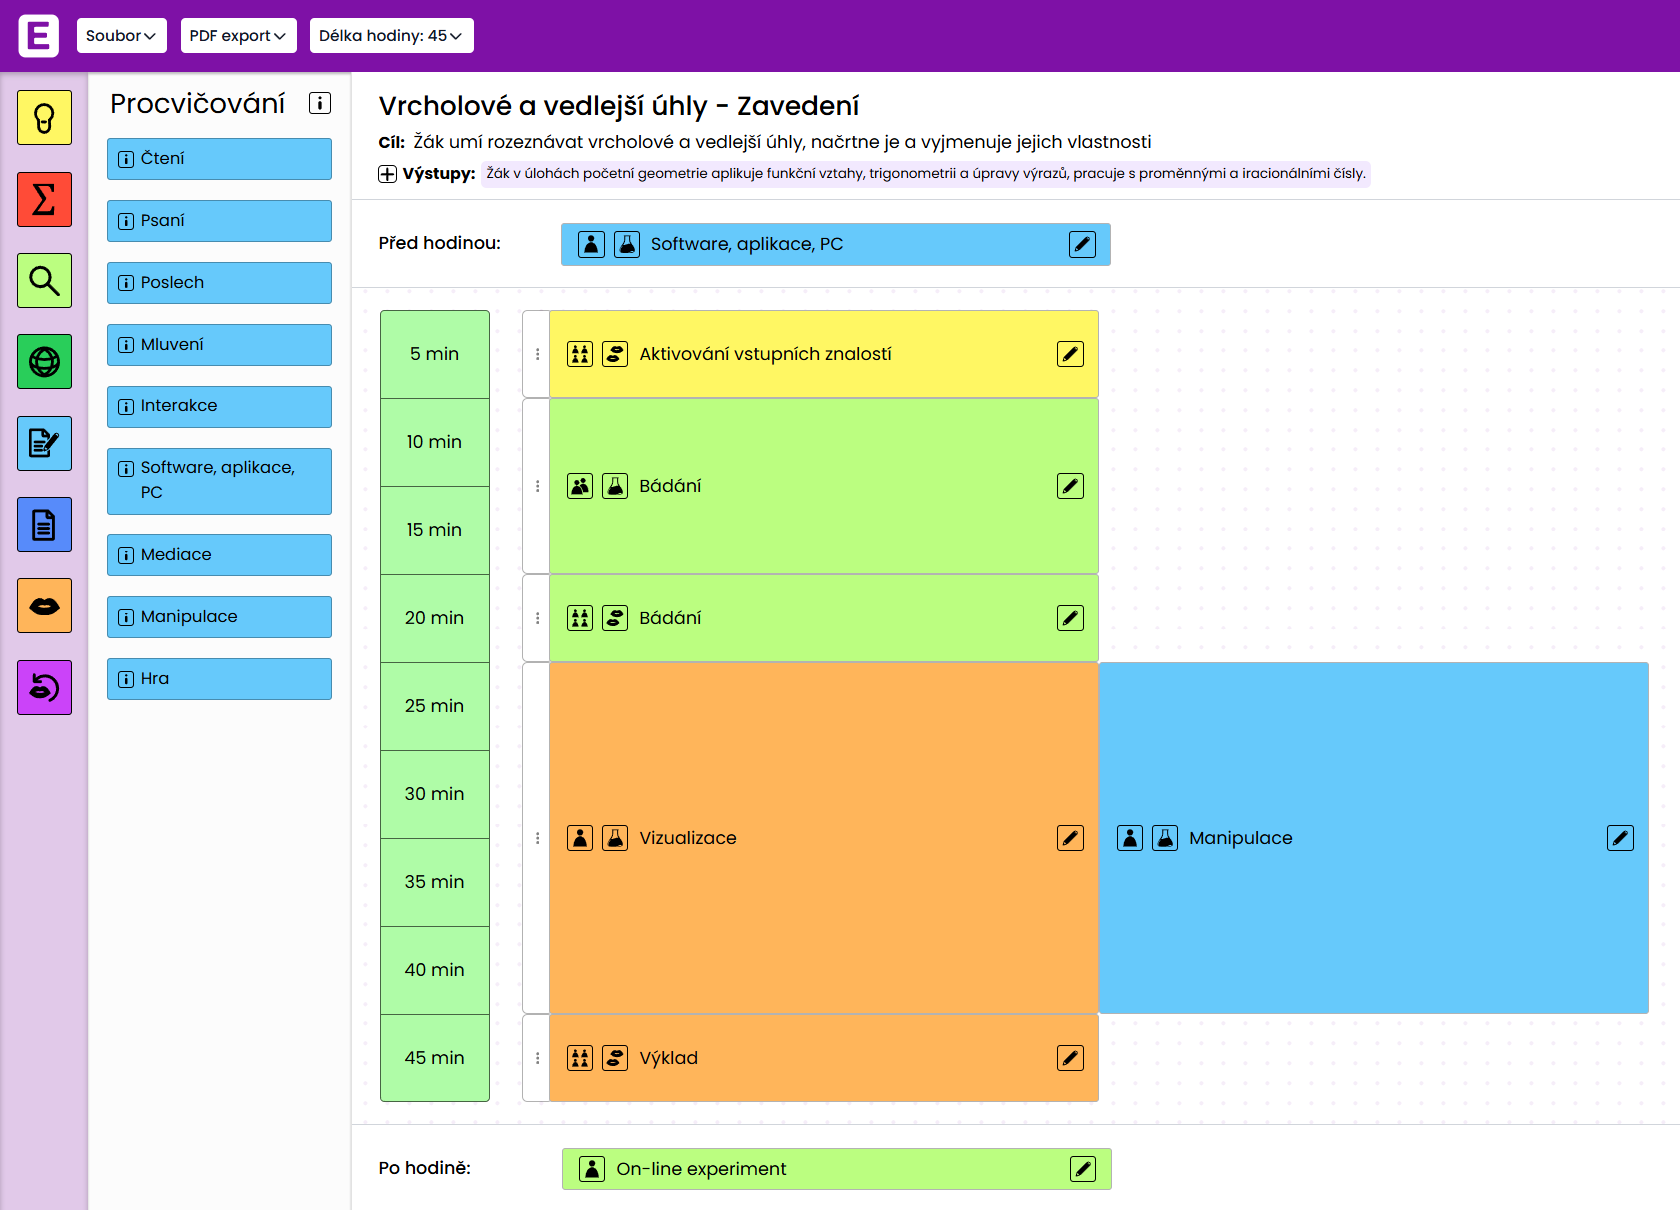
\includegraphics{edubo-1.png}}
	\caption{Okno aplikace \textit{EDUBO} s~náhledem na~editor výukového plánu.}
	\label{fig:edubo-1}
\end{figure}

Editor výukových plánů je klíčovým prvkem softwaru pro plánování výuky, který učitelům umožňuje intuitivně sestavit strukturovaný plán hodiny. Uživatelské rozhraní editoru je přehledné a~usnadňuje práci s~výukovými aktivitami. V~horní části se nachází navigační lišta s~rozbalovacími seznamy, které umožňují manipulaci s~plánem výuky, export do~PDF nebo úpravu délky hodiny.

Na levé straně rozhraní jsou k~dispozici různé typy aktivit, mezi ně patří evokace, hodnocení, objevování, zdroje, procvičování, shrnutí, výklad a~zpětná vazba. Každý z~těchto typů obsahuje další specifické aktivity, které byly vytvořeny ve~spolupráci s~Pedagogickou fakultou Univerzity Karlovy pod vedením proděkana doc.~Antonína Jančaříka. K~jednotlivým aktivitám jsou připojena informační tlačítka, která učitele přesměrují na~podrobné metodické materiály s~návody na~jejich efektivní využití ve~výuce.

Střední část editoru tvoří hlavní plátno, na~kterém učitel vytváří časovou strukturu výuky. Plátno je rozděleno podle časových bloků, do~nichž lze pomocí drag and drop interakce přetahovat vybrané aktivity. Každou aktivitu lze následně editovat, upravit její název, popis či délku a~přidat k~ní potřebné pomůcky, soubory nebo odkazy. Důležitou součástí je také možnost nastavení organizační formy, tedy zda bude aktivita realizována v~rámci celé třídy, ve~skupinách, ve~dvojicích nebo individuálně. Kromě toho je možné určit formu činnosti, například mluvený projev, interakci, čtení, psaní, experiment nebo poslech.

Kromě hlavního plátna obsahuje editor i~speciální sekce pro~aktivity, které mají proběhnout před výukou nebo po~ní. Tento prvek slouží například k~evidenci úkolů, které si žáci mají připravit před hodinou nebo k~záznamu reflexe po~jejím skončení. Editor také podporuje paralelní aktivity, což znamená, že v~jednom časovém úseku mohou probíhat různé činnosti současně. Tato funkce je užitečná například při dělení žáků do~skupin, kdy každá skupina pracuje na~odlišných úkolech.

Další důležitou součástí editoru je sekce věnovaná cílům a~výstupům hodiny. Výstupy vycházejí z~rámcového vzdělávacího programu (RVP), přičemž software umožňuje nejen jejich přizpůsobení, ale také nahrání vlastních výstupů pomocí CSV souboru.

\begin{figure}[H]
	\centering
	\resizebox{12cm}{!}{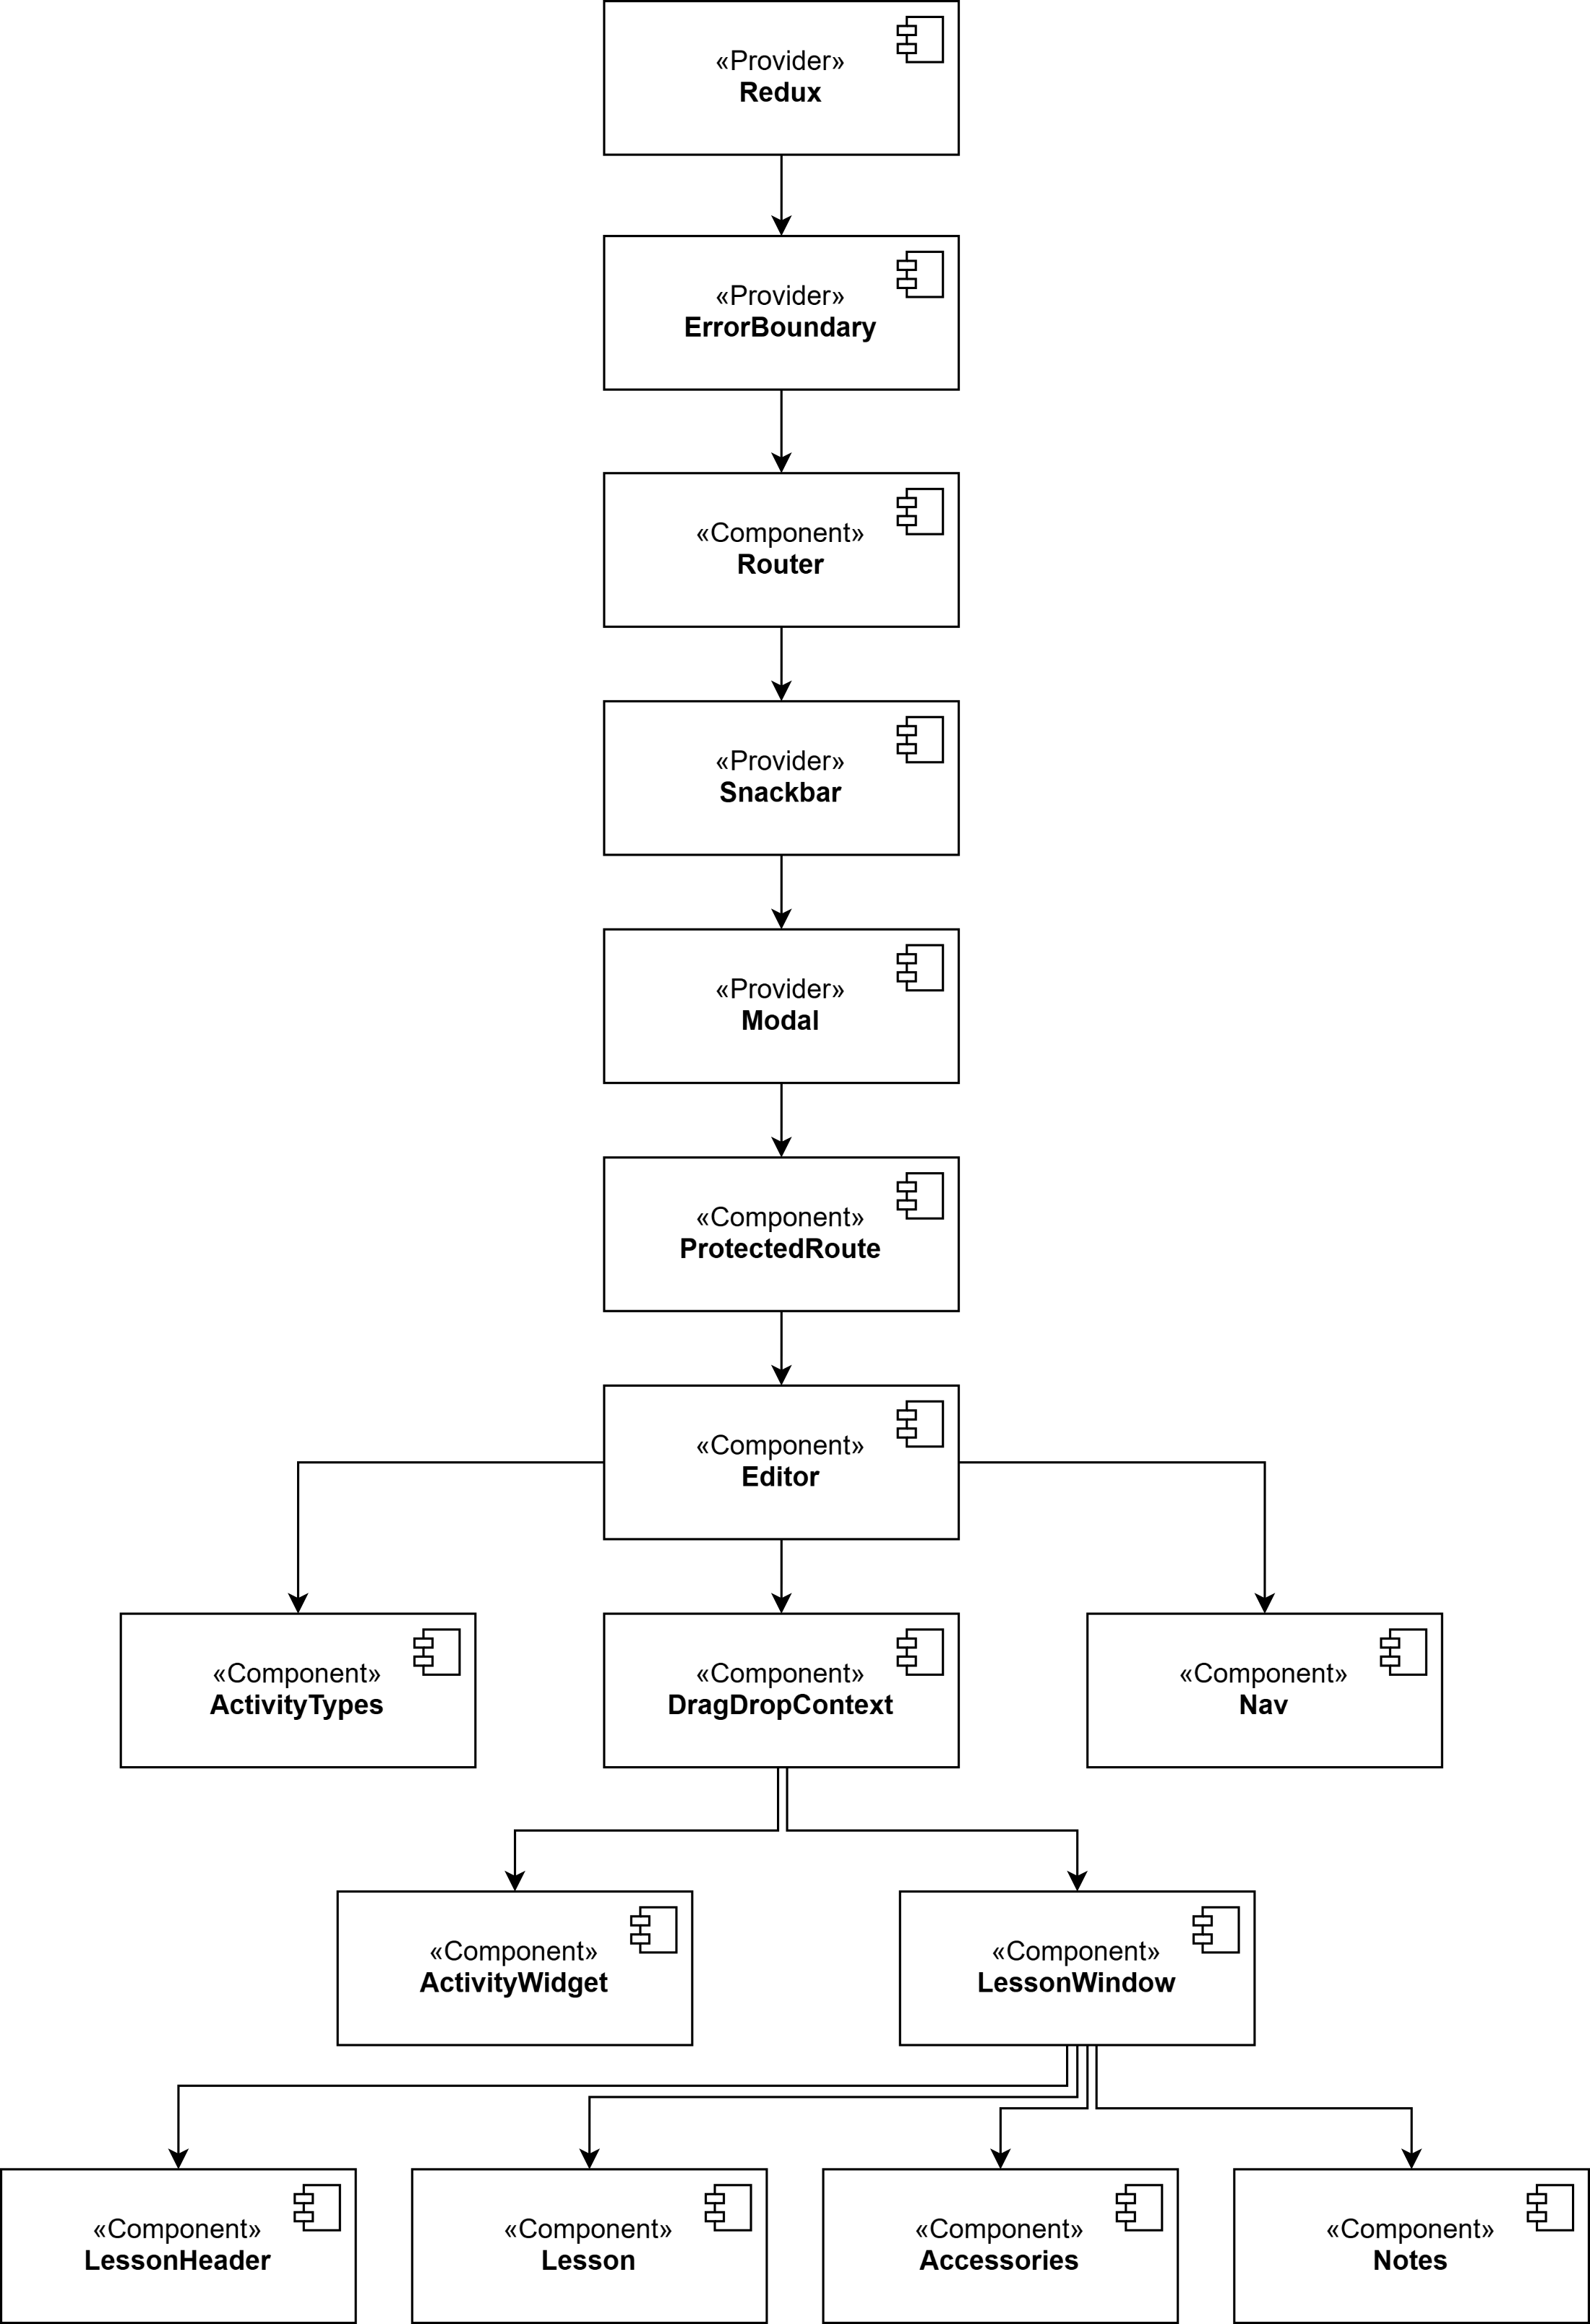
\includegraphics{component-diagram-react-1.png}}
	\caption{Komponentní diagram znázorňující strukturu React komponent v~editoru výukových plánů.}
	\label{fig:component-diagram-react-1}
\end{figure}

\newpage

Tento komponentní diagram znázorňuje strukturu hlavních React komponent v~editoru výukových plánů. Nejvyšší úroveň tvoří globální poskytovatelé (Providers), kteří zajišťují sdílení stavů a~funkcionalit napříč aplikací. \texttt{Redux} spravuje globální stav aplikace, \texttt{ErrorBoundary} se stará o~zachytávání chyb, zatímco \texttt{Snackbar} a~\texttt{Modal} poskytují uživatelské notifikace a~modální okna. \texttt{Router} řídí navigaci mezi stránkami a~\texttt{ProtectedRoute} zajišťuje, že k~editoru mají přístup pouze oprávnění uživatelé.

Jádro editoru tvoří komponenta \texttt{Editor}, která spravuje interaktivní prvky uživatelského rozhraní. Pro správu typu aktivit je využita komponenta \texttt{ActivityTypes}. \texttt{DragDropContext} se stará o~přetahování a~organizaci prvků. Navigační menu je implementováno v~komponentě \texttt{Nav}.

Další klíčové komponenty zahrnují \texttt{LessonWindow}, které představuje hlavní pracovní prostor editoru. V~něm jsou obsaženy komponenty \texttt{LessonHeader} (obsahující název hodiny, cíle a~výstupy), \texttt{Lesson} (hlavní struktura plátna), \texttt{Accessories} (vysouvací okno s~výčtem pomůcek použitých v~plánu) a~\texttt{Notes} (sekce pro dodatečné poznámky učitele). Komponenta \texttt{ActivityWidget} obsahuje jednotlivé výukové aktivity, které lze pomocí drag and drop interakce přetahovat do~plátna editoru, kde jsou následně organizovány podle časové osy výukového plánu.

V~dalších diagramových zobrazeních budou společné komponenty, jako jsou \texttt{Redux},\break\texttt{ErrorBoundary}, \texttt{Router} a~další globální poskytovatelé, vyjmuty, protože tvoří základní infrastrukturu celé aplikace a~nejsou specifické pouze pro~editor. Důraz bude kladen na~detailnější rozdělení jednotlivých částí aplikace dle jejich konkrétní funkcionality.

\subsection{Výukový plán v~PDF formátu}

\begin{figure}[H]
	\centering
	\resizebox{12cm}{!}{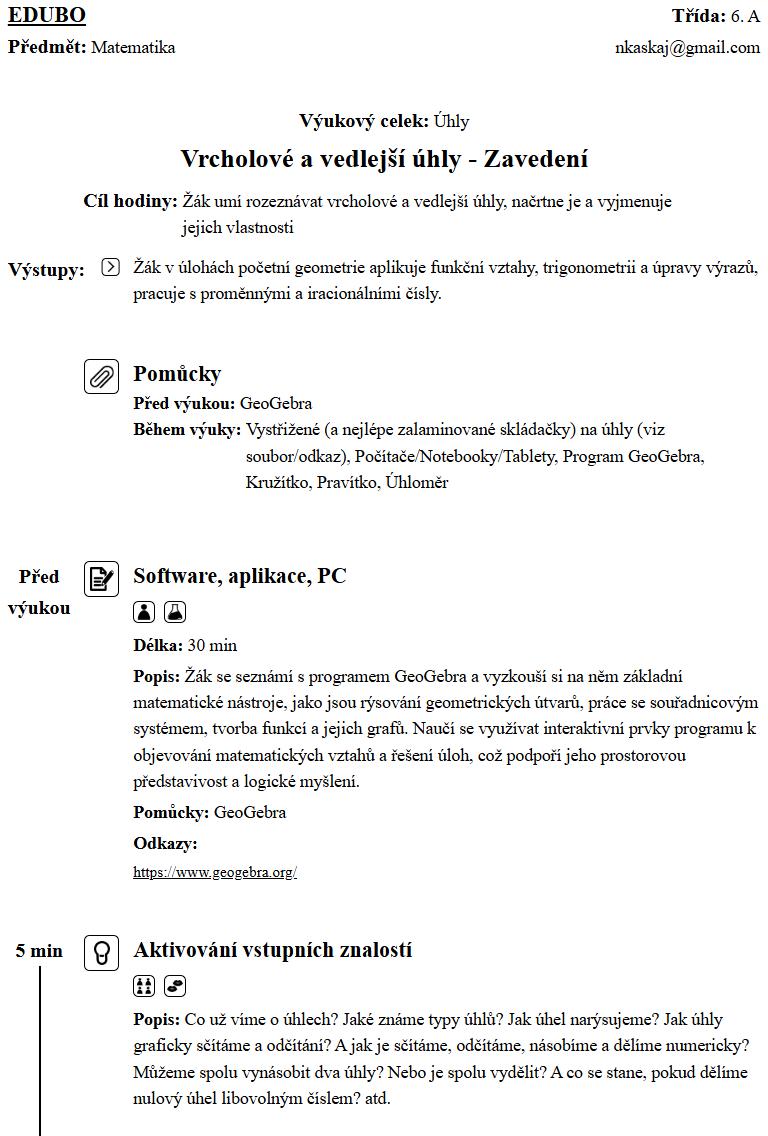
\includegraphics{edubo-2.png}}
	\caption{Ukázka výukového plánu v~PDF formátu.}
	\label{fig:edubo-2}
\end{figure}

Výukový plán lze exportovat do~PDF formátu, což umožňuje učitelům mít snadný přístup k~materiálům i~bez připojení k~internetu. Tento export je generován pomocí HTML šablonového systému Jinja2, který převádí data z~aplikace do~strukturovaného a~čitelného formátu. Výstupní dokument obsahuje všechny důležité informace o~hodině, včetně jejího cíle, výstupů, potřebných pomůcek a~podrobného rozpisu výukových aktivit. Tento formát usnadňuje archivaci a~distribuci plánů mezi učiteli i~studenty.

\newpage

\begin{lstlisting}

 
 
  
   
   
  
  
   
  
  
   <section class="activity">
    <div class="grid grid-cols-24 gap-y-4 mt-12">
     <div class="col-span-2 text-center text-lg font-semibold">
      
       
        <p>{{ total_time.value }} min</p>
       
      
       <p>{{ total_time.value }} min</p>
       <div 
        class="timeline double"
        style="height: calc(100% + 1.25rem);"></div>
      
       <div
        class="timeline double"
        style="height: calc(100% + 3rem);"></div>
      
       <div
        class="timeline double"
        style="height: calc(100% + 3.5rem);"></div>
      
     </div>
    </div>
   </section>
  
 

\end{lstlisting}

Tento úryvek Jinja2 kódu slouží k~vygenerování časové osy v~PDF výukového plánu. Prochází seznam aktivit v~hodině a~postupně sčítá jejich časovou délku. Dynamicky vykresluje minutové značky a~určuje, zda jsou aktivity v~rámci jedné časové jednotky vykonávány paralelně. Pomocí podmínek nastavuje vzhled časové osy, například přidáním dvojité časové linie pro~paralelní aktivity. Výstupem je přehledná vizualizace struktury hodiny se~správným časovým rozvržením jednotlivých aktivit.

\begin{figure}[H]
	\centering
	\resizebox{12cm}{!}{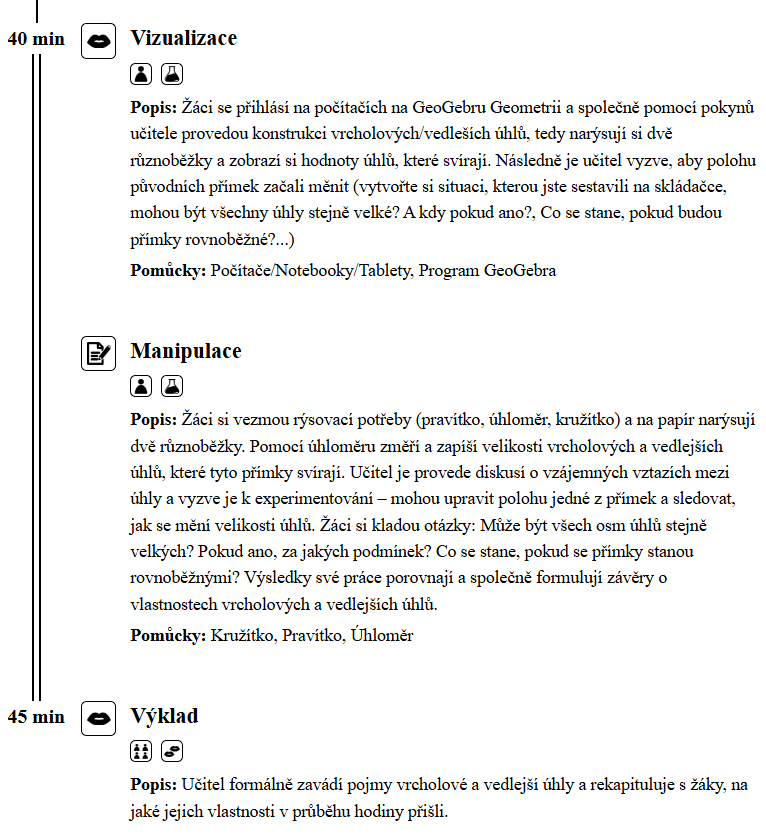
\includegraphics{edubo-3.png}}
	\caption{Ukázka paralelních aktivit ve výukovém plánu v~PDF formátu.}
	\label{fig:edubo-3}
\end{figure}

\begin{lstlisting}
<div class="col-start-3 col-span-2 flex justify-center">
 <img
  src="{{ url_for('static', filename='icons/' + icons.get(activity['color']) + '.png') }}"
  class="activitytype-icon">
</div>
<div class="col-span-20">
 <h1 class="dynamic-header text-xl font-bold">{{ activity.name }}</h1>
 <div class="flex items-baseline my-2">
  
   
    
     <img
      src="{{ url_for('static', filename='activity-icons/' + icon + '.png') }}"
      class="activity-icon">
    
   
  
 </div>
 <div class="flex flex-wrap items-baseline space-x-1 mt-1">
  
   <p>
    <span class="font-bold">Popis: </span>
     {{ html_tags_remover(html_entity_replacer(activity.description)) }}
   </p>
  
 </div>
 <div class="flex items-baseline space-x-1 mt-1">
  
   <span><h1 class="text-base font-semibold">Pomůcky:</h1></span>
   <p>{{ empty_string_remover(activity['gadgets'])|join(', ') }}</p>
  
 </div>
  
  
   <h1 class="text-base font-semibold mt-1">Odkazy:</h1>
  
   
    <p class="text-sm mt-1 underline">{{ url|urlize(target='_blank') }}</p>
   
  
 
</div>
\end{lstlisting}

Tento Jinja2 kód generuje jednotlivé sekce aktivit ve~výukovém plánu PDF. Každá aktivita je vizuálně reprezentována pomocí ikony, názvu, popisu a~případných pomůcek. Kód také dynamicky načítá a~zobrazuje seznam připojených odkazů, pokud jsou k~dispozici. Všechny textové vstupy jsou ošetřeny proti nežádoucím HTML značkám a~speciálním znakům, aby byl výstup čistý a~přehledný.

\subsection{Uživatelské menu}

\begin{figure}[H]
	\centering
	\resizebox{14cm}{!}{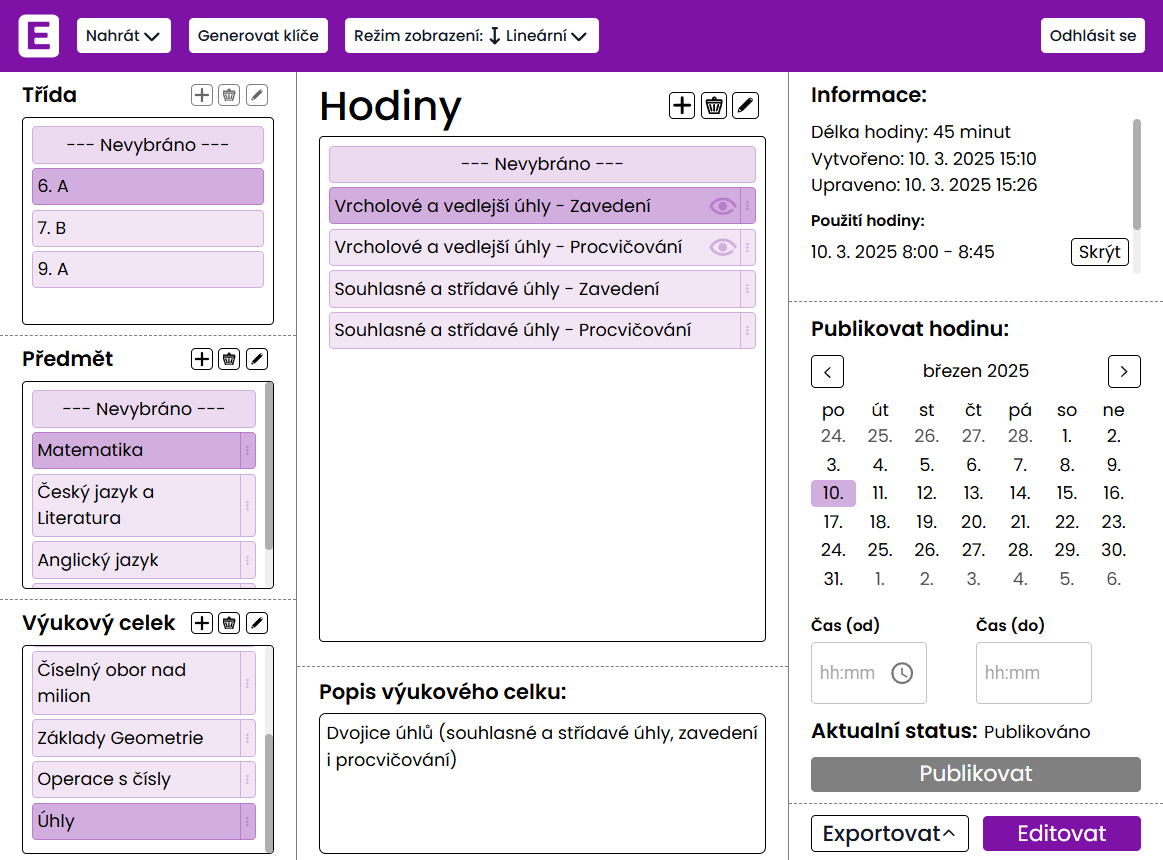
\includegraphics{edubo-4.png}}
	\caption{Okno aplikace \textit{EDUBO} s~náhledem na~uživatelské menu.}
	\label{fig:edubo-4}
\end{figure}

Uživatelské menu poskytuje pedagogům správu a~publikaci výukových plánů. Uživatel může v~navigační liště nahrávat výukové plány, výukové celky nebo soubory výukových celků ve~formátu ZIP, přičemž je podporována integrace s~webovým agregátorem výukových plánů. Dále je možné nahrávat vlastní kurikulární výstupy ve~formátu CSV. Další funkcí je generování registračních klíčů, které studenty automaticky přiřadí do~odpovídajících tříd. Menu také umožňuje změnit režim zobrazení~--~lineární režim, kde uživatel nejprve vybírá třídu a~následně předmět, nebo dynamický režim, kde může být volba předmětu provedena před výběrem třídy.

Uživatelé mají přístup k~seznamům tříd, předmětů, výukových celků a~jednotlivých hodin, přičemž všechny tyto položky mohou přidávat, upravovat a~mazat. Pro~pohodlnou organizaci obsahu je možné využít drag and drop interakce, který usnadňuje řazení výukových položek. Při vytváření třídy lze vybrat z~již existujících tříd a~automaticky se~tak uživatel přiřadí do~dané třídy. V~rámci editace předmětu může pedagog přiřadit již přednastavené kurikulární výstupy nebo nahrát vlastní. Výukové celky je možné doplnit o~poznámky.

\newpage

V~pravé části menu se~nachází informace o~konkrétní hodině spolu s~možností její publikace. Uživatel může nastavit čas a~datum zveřejnění, po~kterém se~daná hodina zobrazí v~uživatelském rozhraní studentů.

\begin{figure}[H]
	\centering
	\resizebox{14cm}{!}{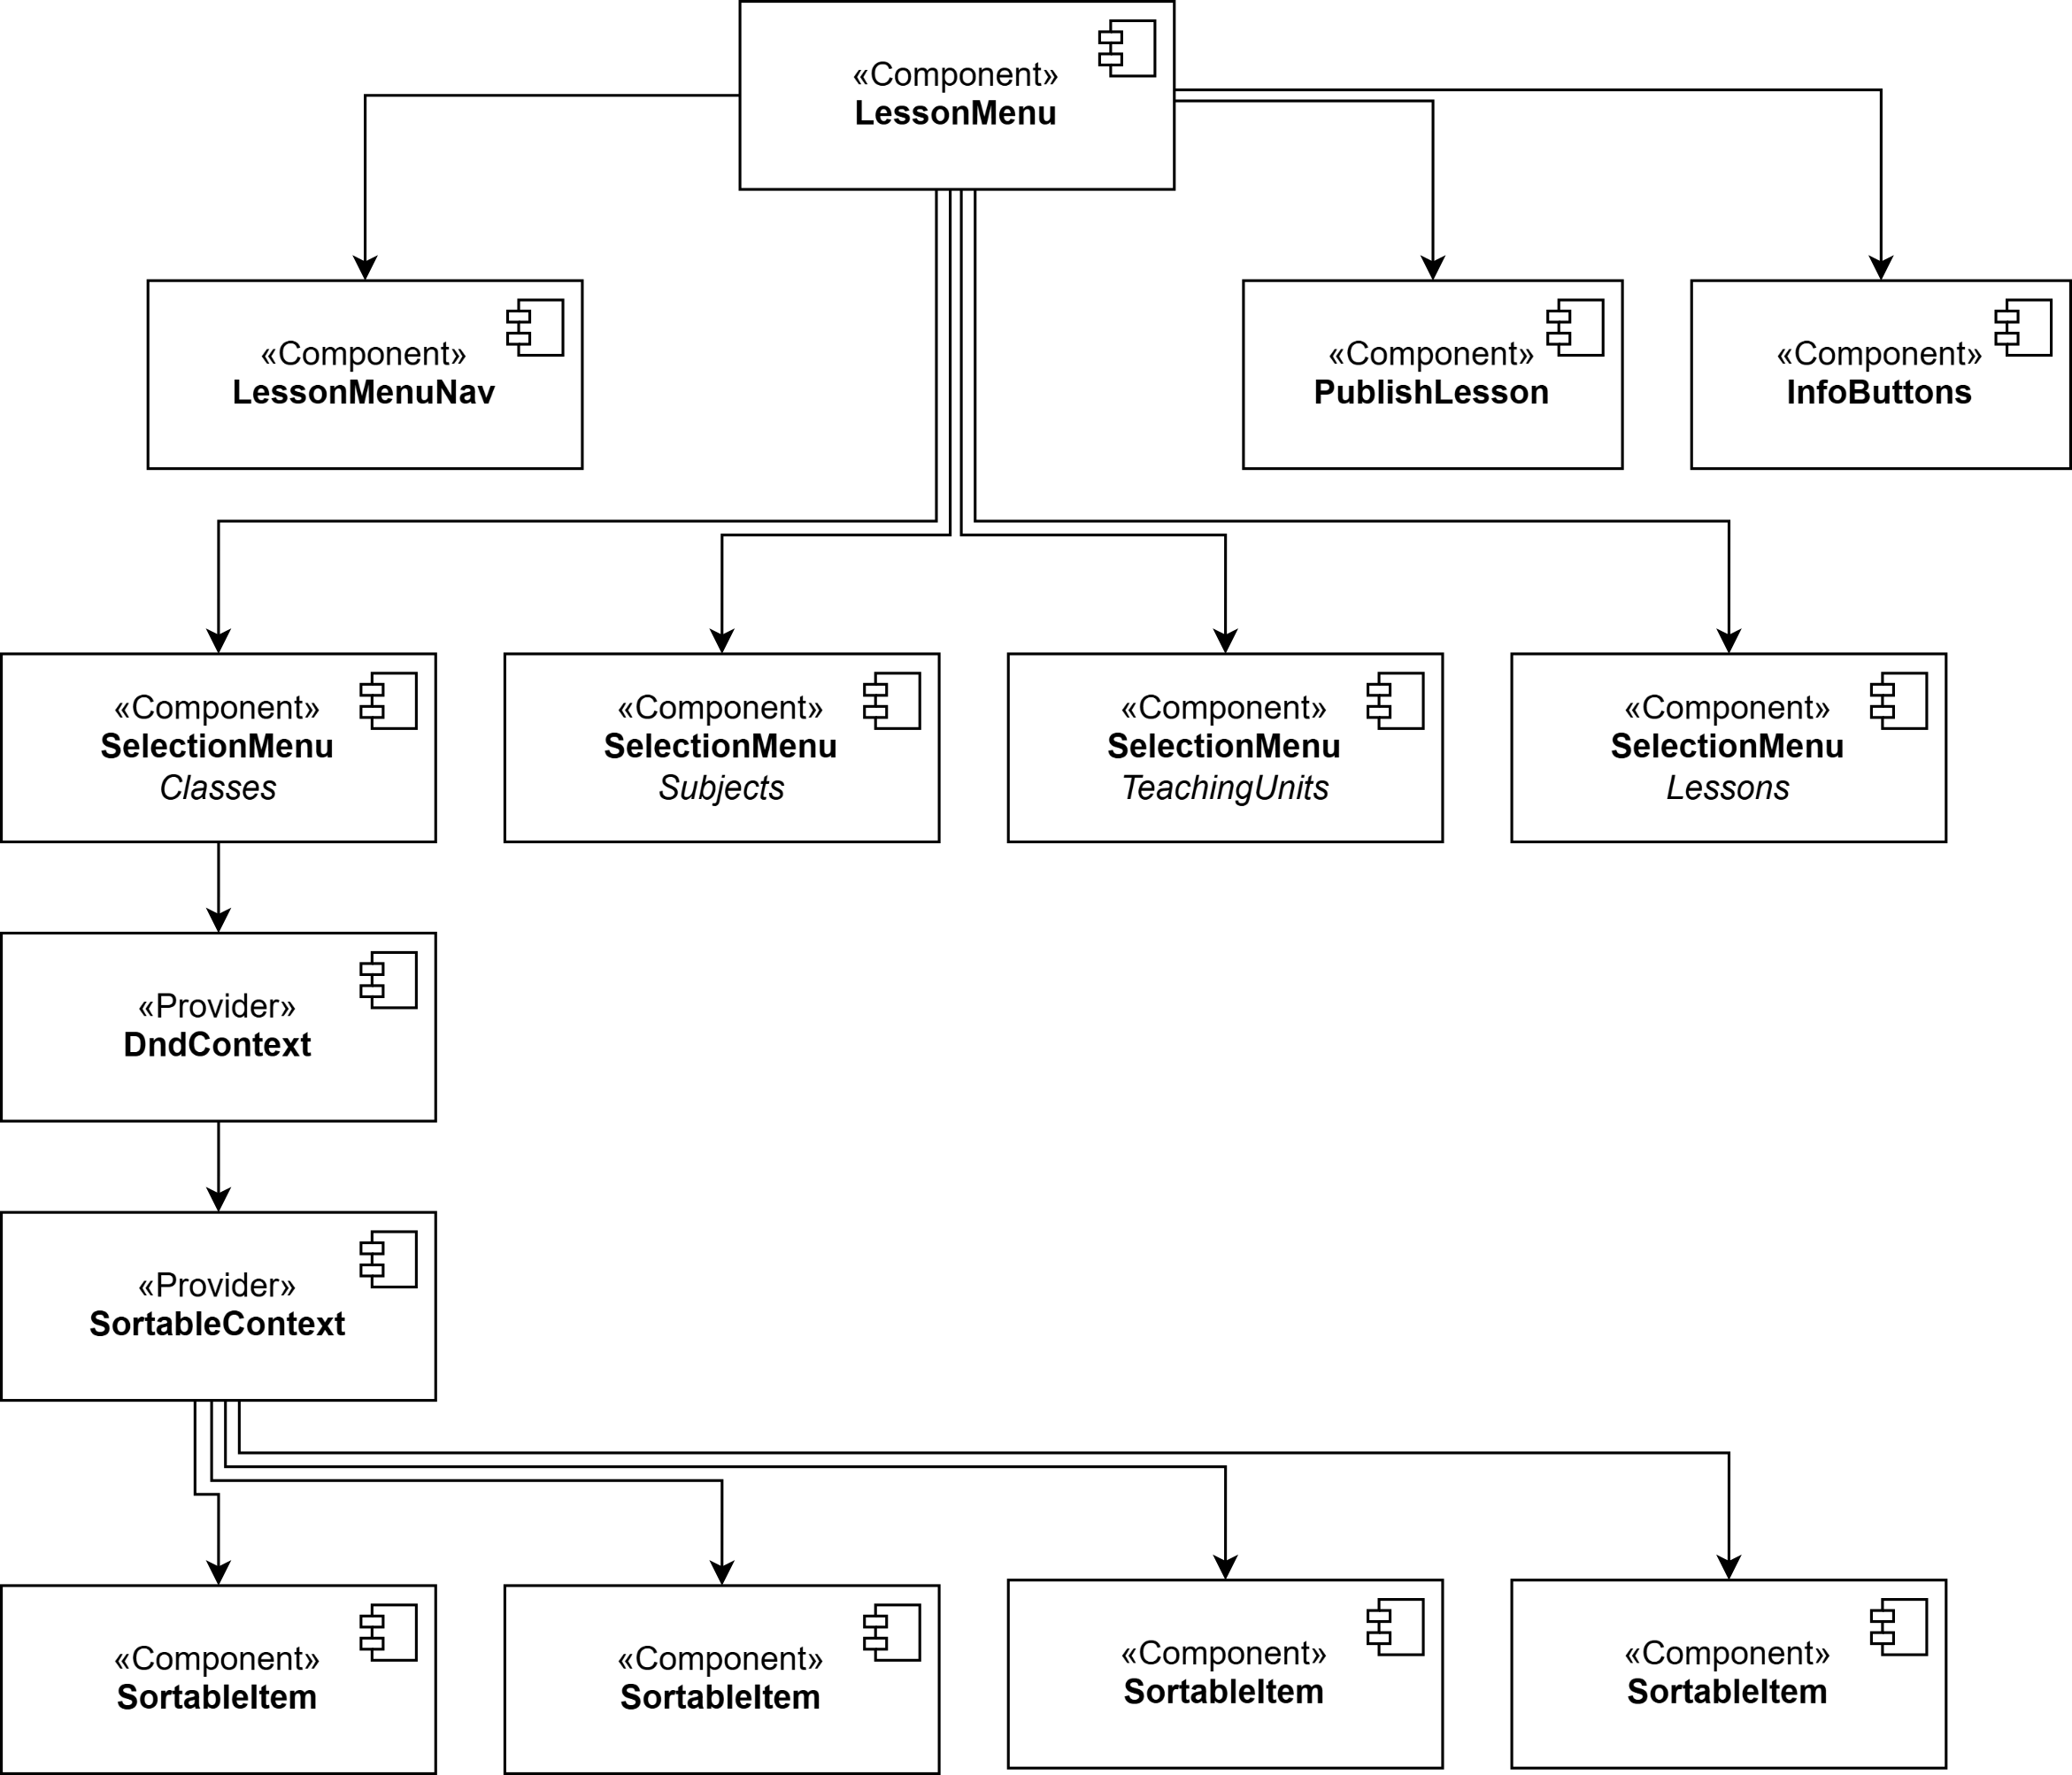
\includegraphics{component-diagram-react-2.png}}
	\caption{Komponentní diagram znázorňující strukturu React komponent v~uživatelském menu.}
	\label{fig:component-diagram-react-2}
\end{figure}

Tento komponentní diagram popisuje strukturu React komponent uživatelského menu v~aplikaci pro~správu výukových plánů. Hlavní komponentou je \texttt{LessonMenu}, která zastřešuje celé rozhraní pro~organizaci tříd, předmětů, výukových celků a~plánů.

Komponenta \texttt{LessonMenuNav} poskytuje navigační prvky pro~orientaci v~menu. \texttt{PublishLesson} umožňuje publikaci výukových plánů a~jejich zpřístupnění studentům. \texttt{InfoButtons} slouží k~zobrazení tlačítek pro~exportování nebo úpravu výukových plánů.

Struktura tříd, předmětů, výukových celků a~plánů je spravována pomocí komponent\break\texttt{SelectionMenu}, které jsou rozděleny podle jednotlivých kategorií (\texttt{Classes}, \texttt{Subjects},\break\texttt{TeachingUnits} a~\texttt{Lessons}). Tyto komponenty umožňují uživateli vybírat a~spravovat jednotlivé položky.

Pro~podporu drag and drop interakce byly do~menu integrovány providery \texttt{DndContext}\break a~\texttt{SortableContext}, které umožňují přetahování a~řazení prvků. Samotné přetahovatelné položky jsou reprezentovány komponentou \texttt{SortableItem}, která se~stará o~jejich správné zobrazení a~interaktivitu v~rámci menu.

% TODO: TADY ZMĚNIT KÓD JESTLI TO BUDE KÓD %
\begin{lstlisting}
const modalAddLessonCallback = async (oldValue: string) => {
 const value = oldValue.trim();
 if (!userData) return console.error("UserData are missing!");
 if (value === "") return openErrorSnackbar("Hodina musí mít název!");
 if (value.length > 63) return openErrorSnackbar("Název nesmí být delší než 63 znaků!");

 const newUserData: iUserData = JSON.parse(JSON.stringify(userData));
	
 const indexes = getActiveItemsIndexes();
 const lessons = newUserData
  .classes[indexes.activeClassIndex]
  .subjects[indexes. activeSubjectIndex]
  .teaching_units[indexes.activeTeachingUnitIndex]
  .lessons;
	
 if (lessons.find((item) => (item.name === value)))
  return openErrorSnackbar("Hodina se stejným názvem již existuje!");
	
 const newLesson: iMenuLesson = {
  _id: uuidv4(),
  name: value,
  published: false,
  days_of_usage: []
 };
 lessons.push(newLesson);

 await Promise.all([
  updateClasses(newUserData.classes),
  updateLesson(newLesson._id, newLesson.name)
 ]);
};
\end{lstlisting}

Tato funkce je určena k~vytvoření nového výukového plánu. Jejím parametrem je řetězec představující název nového plánu. Na začátku probíhá kontrola, zda zadaný název splňuje všechny potřebné podmínky, jako je prázdný název nebo překročení maximální délky. Následně se vytvoří kopie uživatelských dat, která je připravena pro další úpravy.

Funkce dále získá aktivní indexy, tedy index aktuálně vybrané třídy, předmětu a~výukového celku. Na základě těchto indexů se vytvoří reference na příslušné pole výukových plánů, kde bude nový výukový plán přidán. Před přidáním se zkontroluje, zda již v~datech neexistuje výukový plán se~stejným názvem, aby nedošlo k~duplicitě.

\newpage

Pokud je kontrola úspěšná, vytvoří se objekt nového výukového plánu s~unikátním identifikátorem, názvem a~výchozími hodnotami pro další vlastnosti. Tento objekt je následně přidán do~pole výukových plánů.

Na závěr funkce vytvoří \texttt{Promise} (JavaScriptový příslib), který zajistí paralelní odeslání dvou požadavků na backend. První požadavek aktualizuje uživatelská data v~databázi, zatímco druhý vytvoří novou instanci výukového plánu v~databázi. Tento postup zajišťuje synchronizaci mezi lokálními daty a~databází a~umožňuje správnou funkčnost aplikace.

\subsubsection{Uživatelské rozhraní studenta}

Uživatelské rozhraní studenta je navrženo tak, aby umožňovalo snadný přístup k~výukovým plánům a~organizaci výukových hodin. Studenti mají k~dispozici dvě hlavní zobrazení~--~\textbf{Kalendář} a~\textbf{Předměty}.

\begin{figure}[H]
	\centering
	\resizebox{10cm}{!}{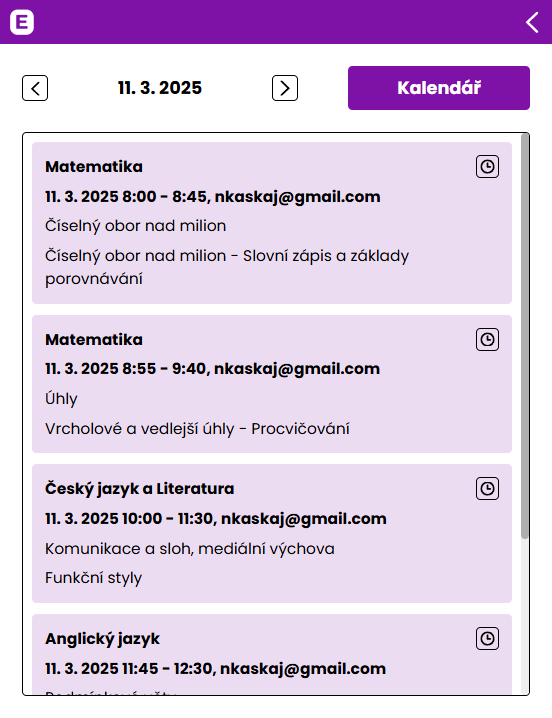
\includegraphics{edubo-5.png}}
	\caption{Mobilní zobrazení aplikace \textit{EDUBO} s~náhledem na~kalendář studenta.}
	\label{fig:edubo-5}
\end{figure}

\newpage

V~zobrazení \textbf{Kalendář} se zobrazují všechny naplánované výukové hodiny pro vybraný den. Každá hodina obsahuje informace o~předmětu, čase, vyučujícím a~tematickém zaměření výukové hodiny. Studenti si mohou přepínat mezi jednotlivými dny pomocí navigačních tlačítek nebo otevřít kalendář a~zvolit libovolné datum, pro které chtějí zobrazit výuku.

\begin{figure}[H]
	\centering
	\resizebox{10cm}{!}{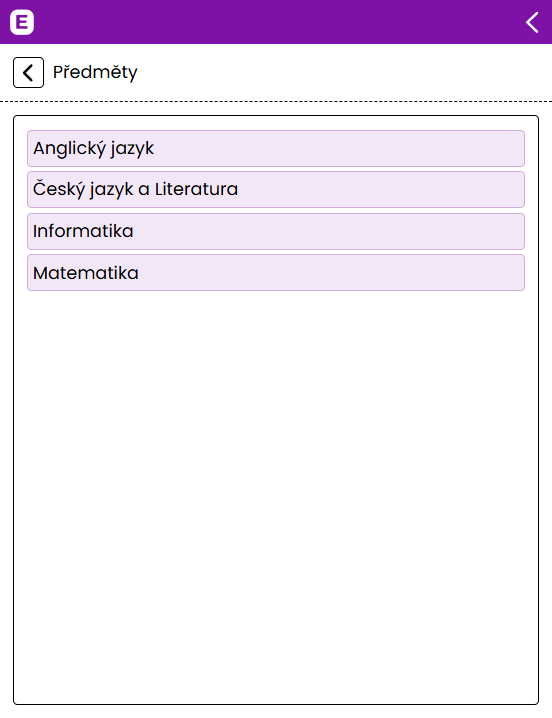
\includegraphics{edubo-6.png}}
	\caption{Mobilní zobrazení aplikace \textit{EDUBO} s~náhledem na~předměty studenta.}
	\label{fig:edubo-6}
\end{figure}

Zobrazení \textbf{Předměty} poskytuje přehled všech předmětů, ke~kterým má student přístup na~základě publikovaných výukových hodin. Po kliknutí na~konkrétní předmět se zobrazí výukové celky daného předmětu, které student může dále rozkliknout pro zobrazení jednotlivých výukových hodin.

\begin{figure}[H]
	\centering
	\resizebox{10cm}{!}{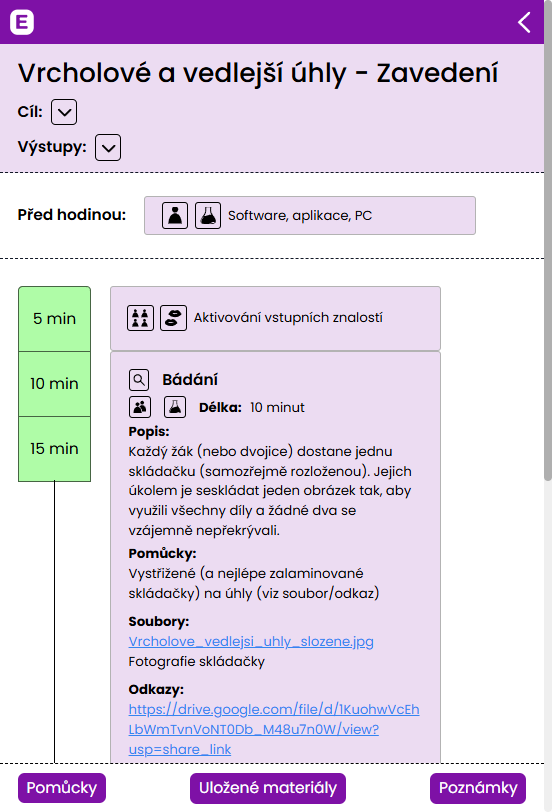
\includegraphics{edubo-7.png}}
	\caption{Mobilní zobrazení aplikace \textit{EDUBO} s~náhledem na~výukový plán.}
	\label{fig:edubo-7}
\end{figure}

Zobrazení výukové lekce poskytuje studentům přehledný a~interaktivní způsob, jak se seznámit s~výukovým plánem dané výukové lekce. V~horní části okna se nachází název výukové lekce, její cíle a~očekávané kurikulární výstupy. Tyto informace umožňují studentům pochopit hlavní zaměření výukové lekce a~to, co se očekává, že se během ní naučí.

Pod tímto úvodním blokem se nachází samotný časový plán výukové lekce. Struktura je rozdělena do~tří částí: \textbf{Před hodinou}, kde se nacházejí aktivity určené k~přípravě před výukou, \textbf{Samotná hodina}, obsahující všechny naplánované činnosti, a~\textbf{Po hodině}, která zahrnuje následné aktivity k~upevnění učiva. Aktivity jsou vizuálně rozděleny podle délky trvání a~po kliknutí na~konkrétní aktivitu se rozbalí její detailní popis, včetně pomůcek, přiložených souborů a~odkazů na~online zdroje.

Ve spodní části obrazovky se nachází tři hlavní tlačítka. \textbf{Pomůcky} zobrazí seznam všech potřebných pomůcek pro danou výukovou lekci. \textbf{Uložené materiály} umožní přístup ke~všem souborům a~odkazům, které jsou součástí výuky. \textbf{Poznámky} poskytují doplňující informace k~výukovému plánu, které mohou učitelé přidat pro lepší porozumění a~přípravu na~výukovou lekci.


\section{Implementace webového agregátoru výukových plánů}

Během vývoje webového agregátoru výukových plánů bylo nutné navrhnout a~implementovat platformu, která umožní učitelům efektivně sdílet své výukové plány vytvořené v~aplikaci \textit{EDUBO}. Hlavním cílem bylo vytvořit intuitivní webovou aplikaci, která nabídne pokročilé vyhledávání a~filtrování plánů podle různých kritérií, možnost jejich stažení a~hodnocení. Důležitou součástí systému bylo také umožnit učitelům přidávat alternativní či upravené verze výukových plánů a~tím podpořit spolupráci v~pedagogické komunitě. Vývoj probíhal ve~spolupráci se~společností Mr.~Cloud~s.r.o., která poskytla odborné konzultace a~podporu při návrhu architektury aplikace.

\subsection{Vývojový proces a týmová spolupráce}

Třetí iterace projektu byla zaměřena na~vývoj webového agregátoru výukových plánů, který umožňuje učitelům sdílet a~spravovat výukové materiály. Tato část vývoje probíhala pod vedením projektového manažera \textbf{Lukáše Polidara}, který měl na~starosti organizaci práce, komunikaci se~stakeholdery a~koordinaci vývojového týmu. Roli Scrum mastera jsem v~rámci týmu zastával já. Byl jsem zodpovědný za~efektivní fungování týmu podle agilní metodiky Scrum, vedení sprintů a~dohled nad~dodržováním vývojového postupu.

Hlavní frontendový vývoj vedl \textbf{Lukáš Priban}, který koordinoval práci na~uživatelském rozhraní aplikace. Spolu s~ním na~frontendu pracovali \textbf{Andrej Dunda}, \textbf{Vlasta Michalcová} a~\textbf{Tomáš Svoboda}, který měl zároveň na~starosti testování aplikace. Backendovou část vývoje měl na~starosti hlavní backend programátor \textbf{Jakub Kopecký}, který zodpovídal za~návrh a~implementaci aplikační logiky a~komunikaci s~databází. Na~rozdíl od~předchozích iterací nebyl UI/UX návrh (návrh uživatelského rozhraní a~uživatelského zážitku) zpracován interně, ale byl vytvořen UI/UX designérem společnosti Mr.~Cloud~s.r.o., který připravil návrh uživatelského rozhraní ve~Figma včetně funkčního prototypu.

Metodika vývoje, komunikace a~správa verzí zůstaly stejné jako v~předchozích iteracích. Hlavním nástrojem pro komunikaci byl Discord, kde probíhaly pravidelné stand-up meetingy, hodnotící pokrok a~plánující další kroky. Pro řízení úkolů a~sledování postupu práce byla využívána Kanban tabule v~ClickUpu. Verzování kódu probíhalo pomocí softwaru Git na~platformě GitHub, kde bylo dodržováno standardizované pojmenovávání větví, pull requesty a~code review.

\subsection{Návrh uživatelského rozhraní ve Figma}

Návrh uživatelského rozhraní ve~Figma byl klíčovým podkladem pro vývoj webového agregátoru výukových plánů. Byl nám předán na~začátku třetí iterace a~obsahoval funkční prototyp, což umožnilo interaktivní náhled na~plánovanou podobu aplikace. Díky této funkcionalitě si vývojáři mohli rozhraní předem proklikat a~otestovat, což pomohlo s~lepším pochopením způsobu, jakým uživatelé interagují s~aplikací, a~usnadnilo implementaci.

Kromě samotného prototypu obsahoval návrh kompletní dokumentaci designu, tedy definované barvy, fonty, tlačítka a~všechny potřebné UI komponenty. Tato strukturovaná dokumentace výrazně urychlila vývoj, protože umožnila nejdříve vytvořit základní vizuální komponenty a~styly, které bylo následně možné znovu využít v~celém projektu.

Přestože návrh ve~Figma tvořil pevný základ, výsledná aplikace není identická s~původním designem. Během vývoje se totiž objevily nové požadavky a~funkcionality, které bylo nutné přidat nebo upravit. Některé části návrhu bylo proto nutné rozšířit nebo modifikovat, aby odpovídaly reálným potřebám uživatelů.

\begin{figure}[H]
	\centering
	\resizebox{16cm}{!}{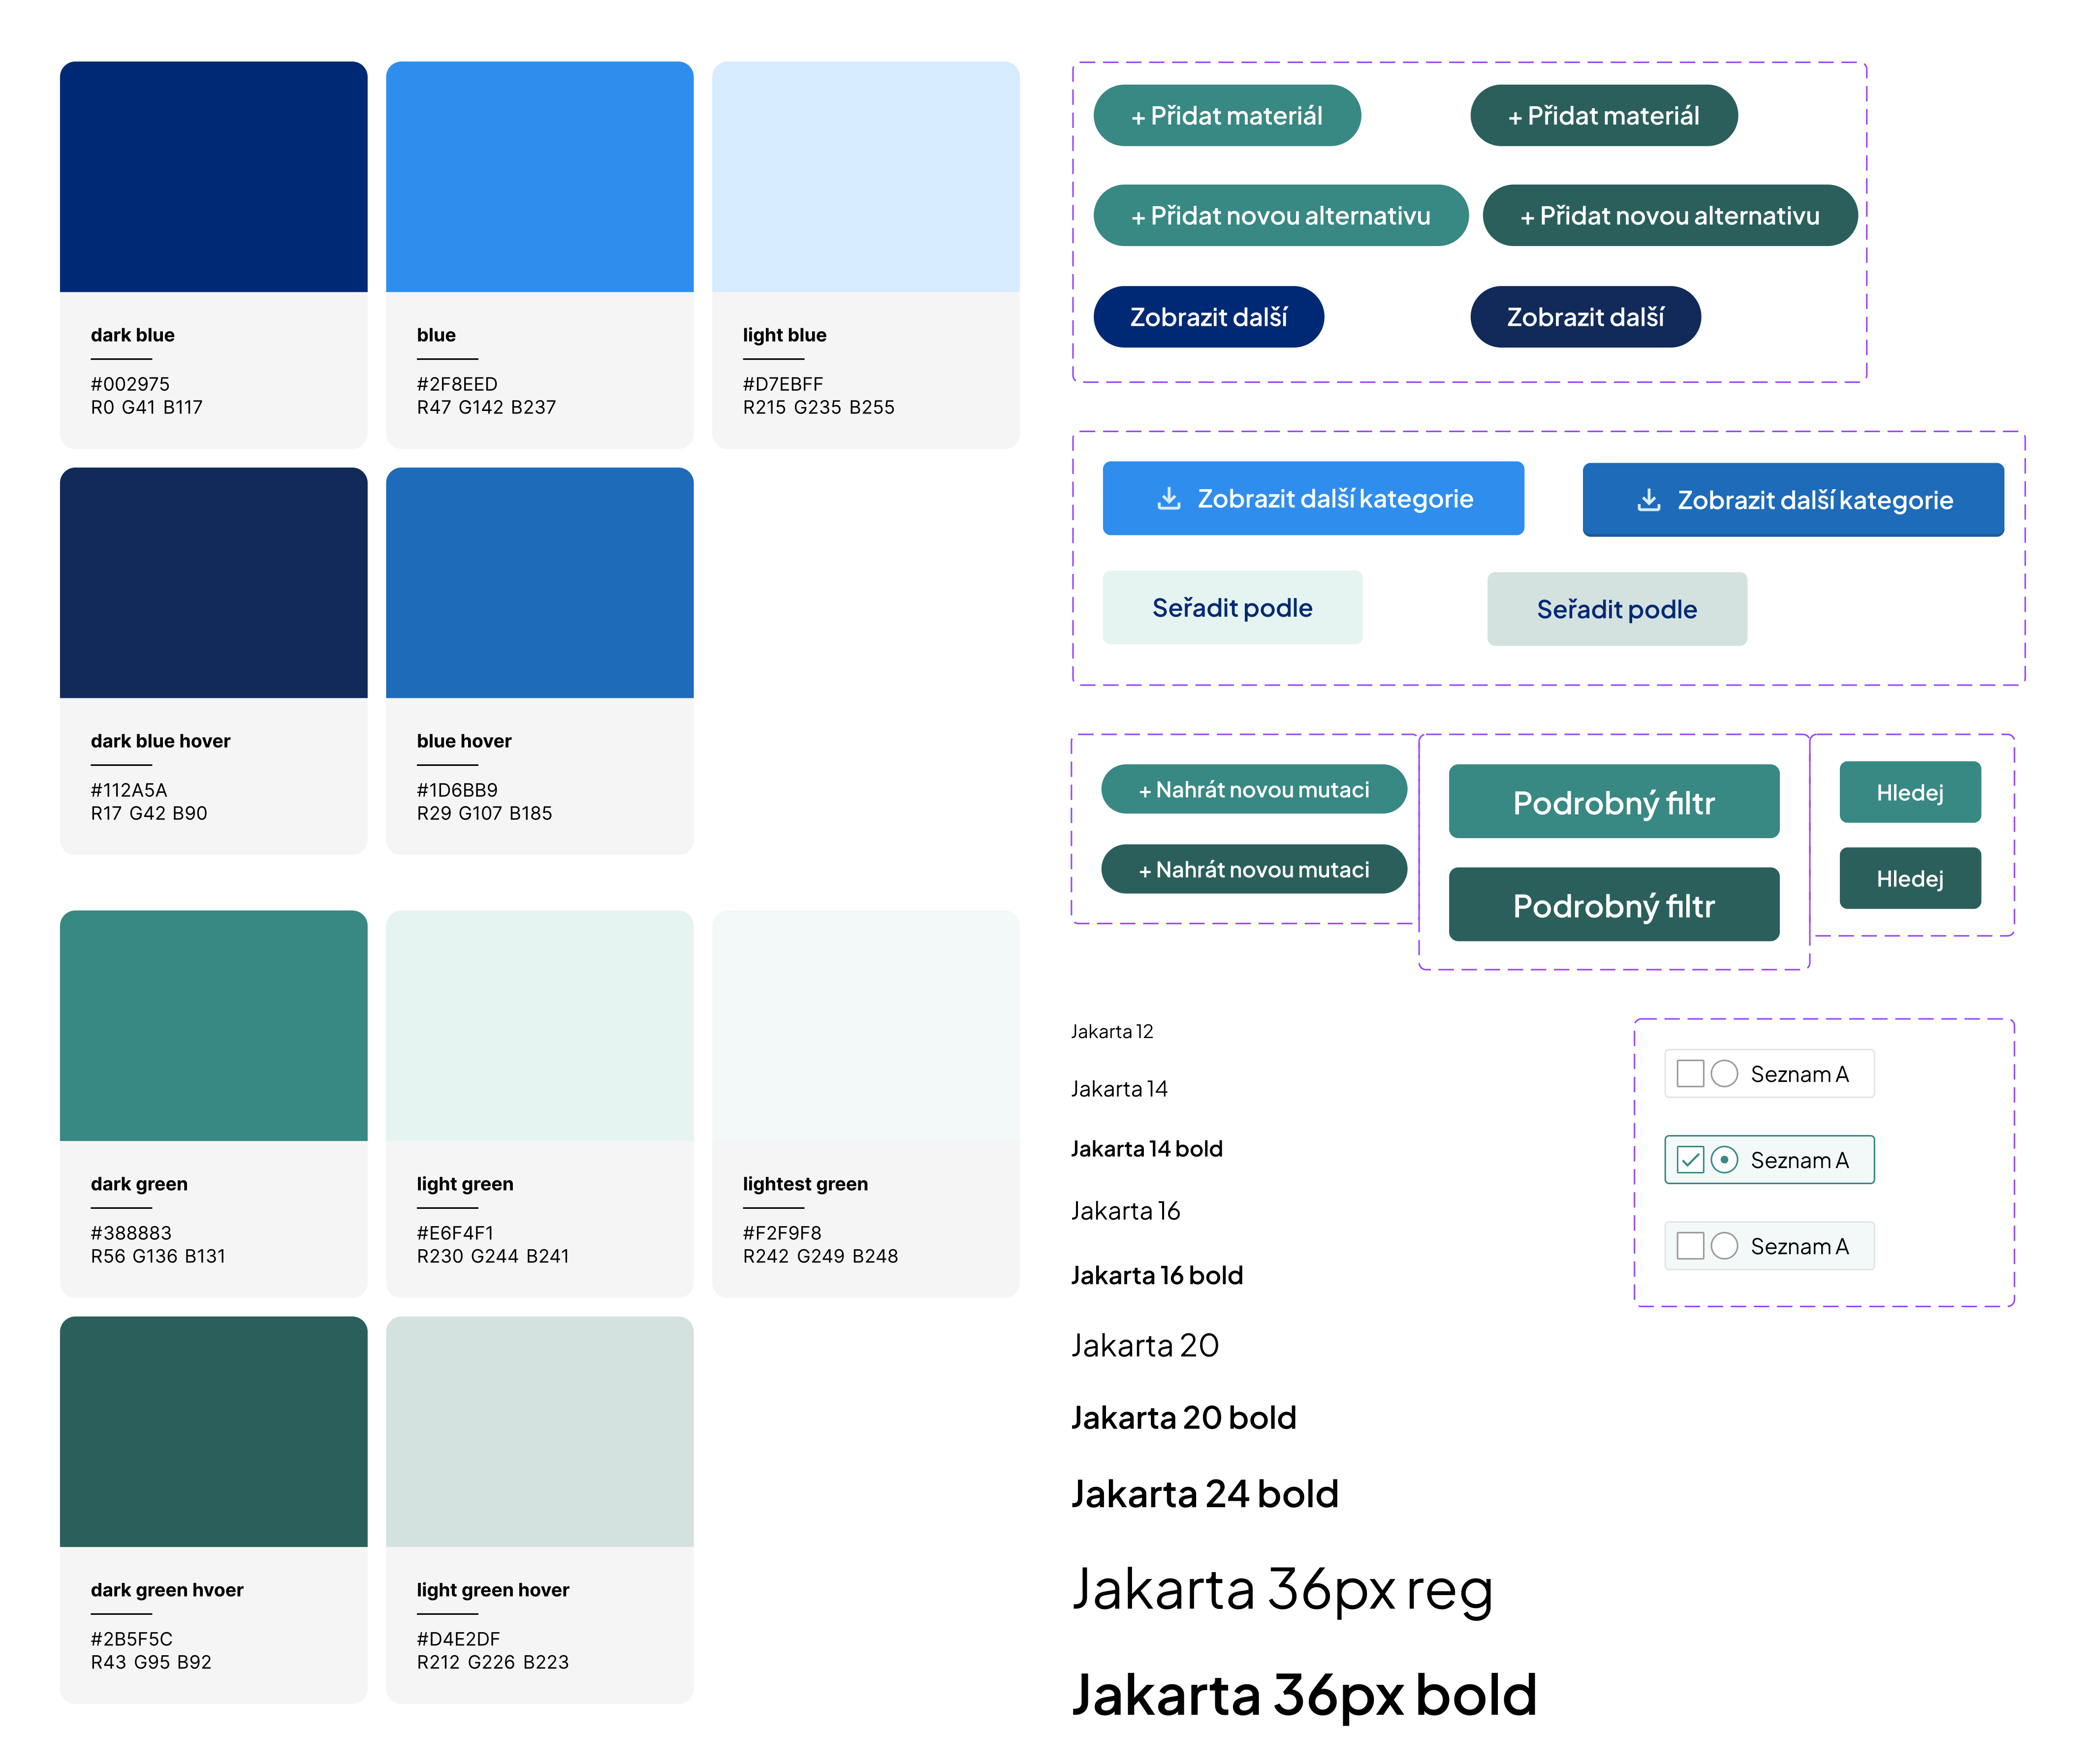
\includegraphics{eduklub-navrh-1.png}}
	\caption{Dokumentace návrhu uživatelského rozhraní v~aplikaci Figma\break pro~\textit{Eduklub~--~plány výuky}.}
	\label{fig:eduklub-navrh-1}
\end{figure}

\begin{figure}[H]
	\centering
	\resizebox{16cm}{!}{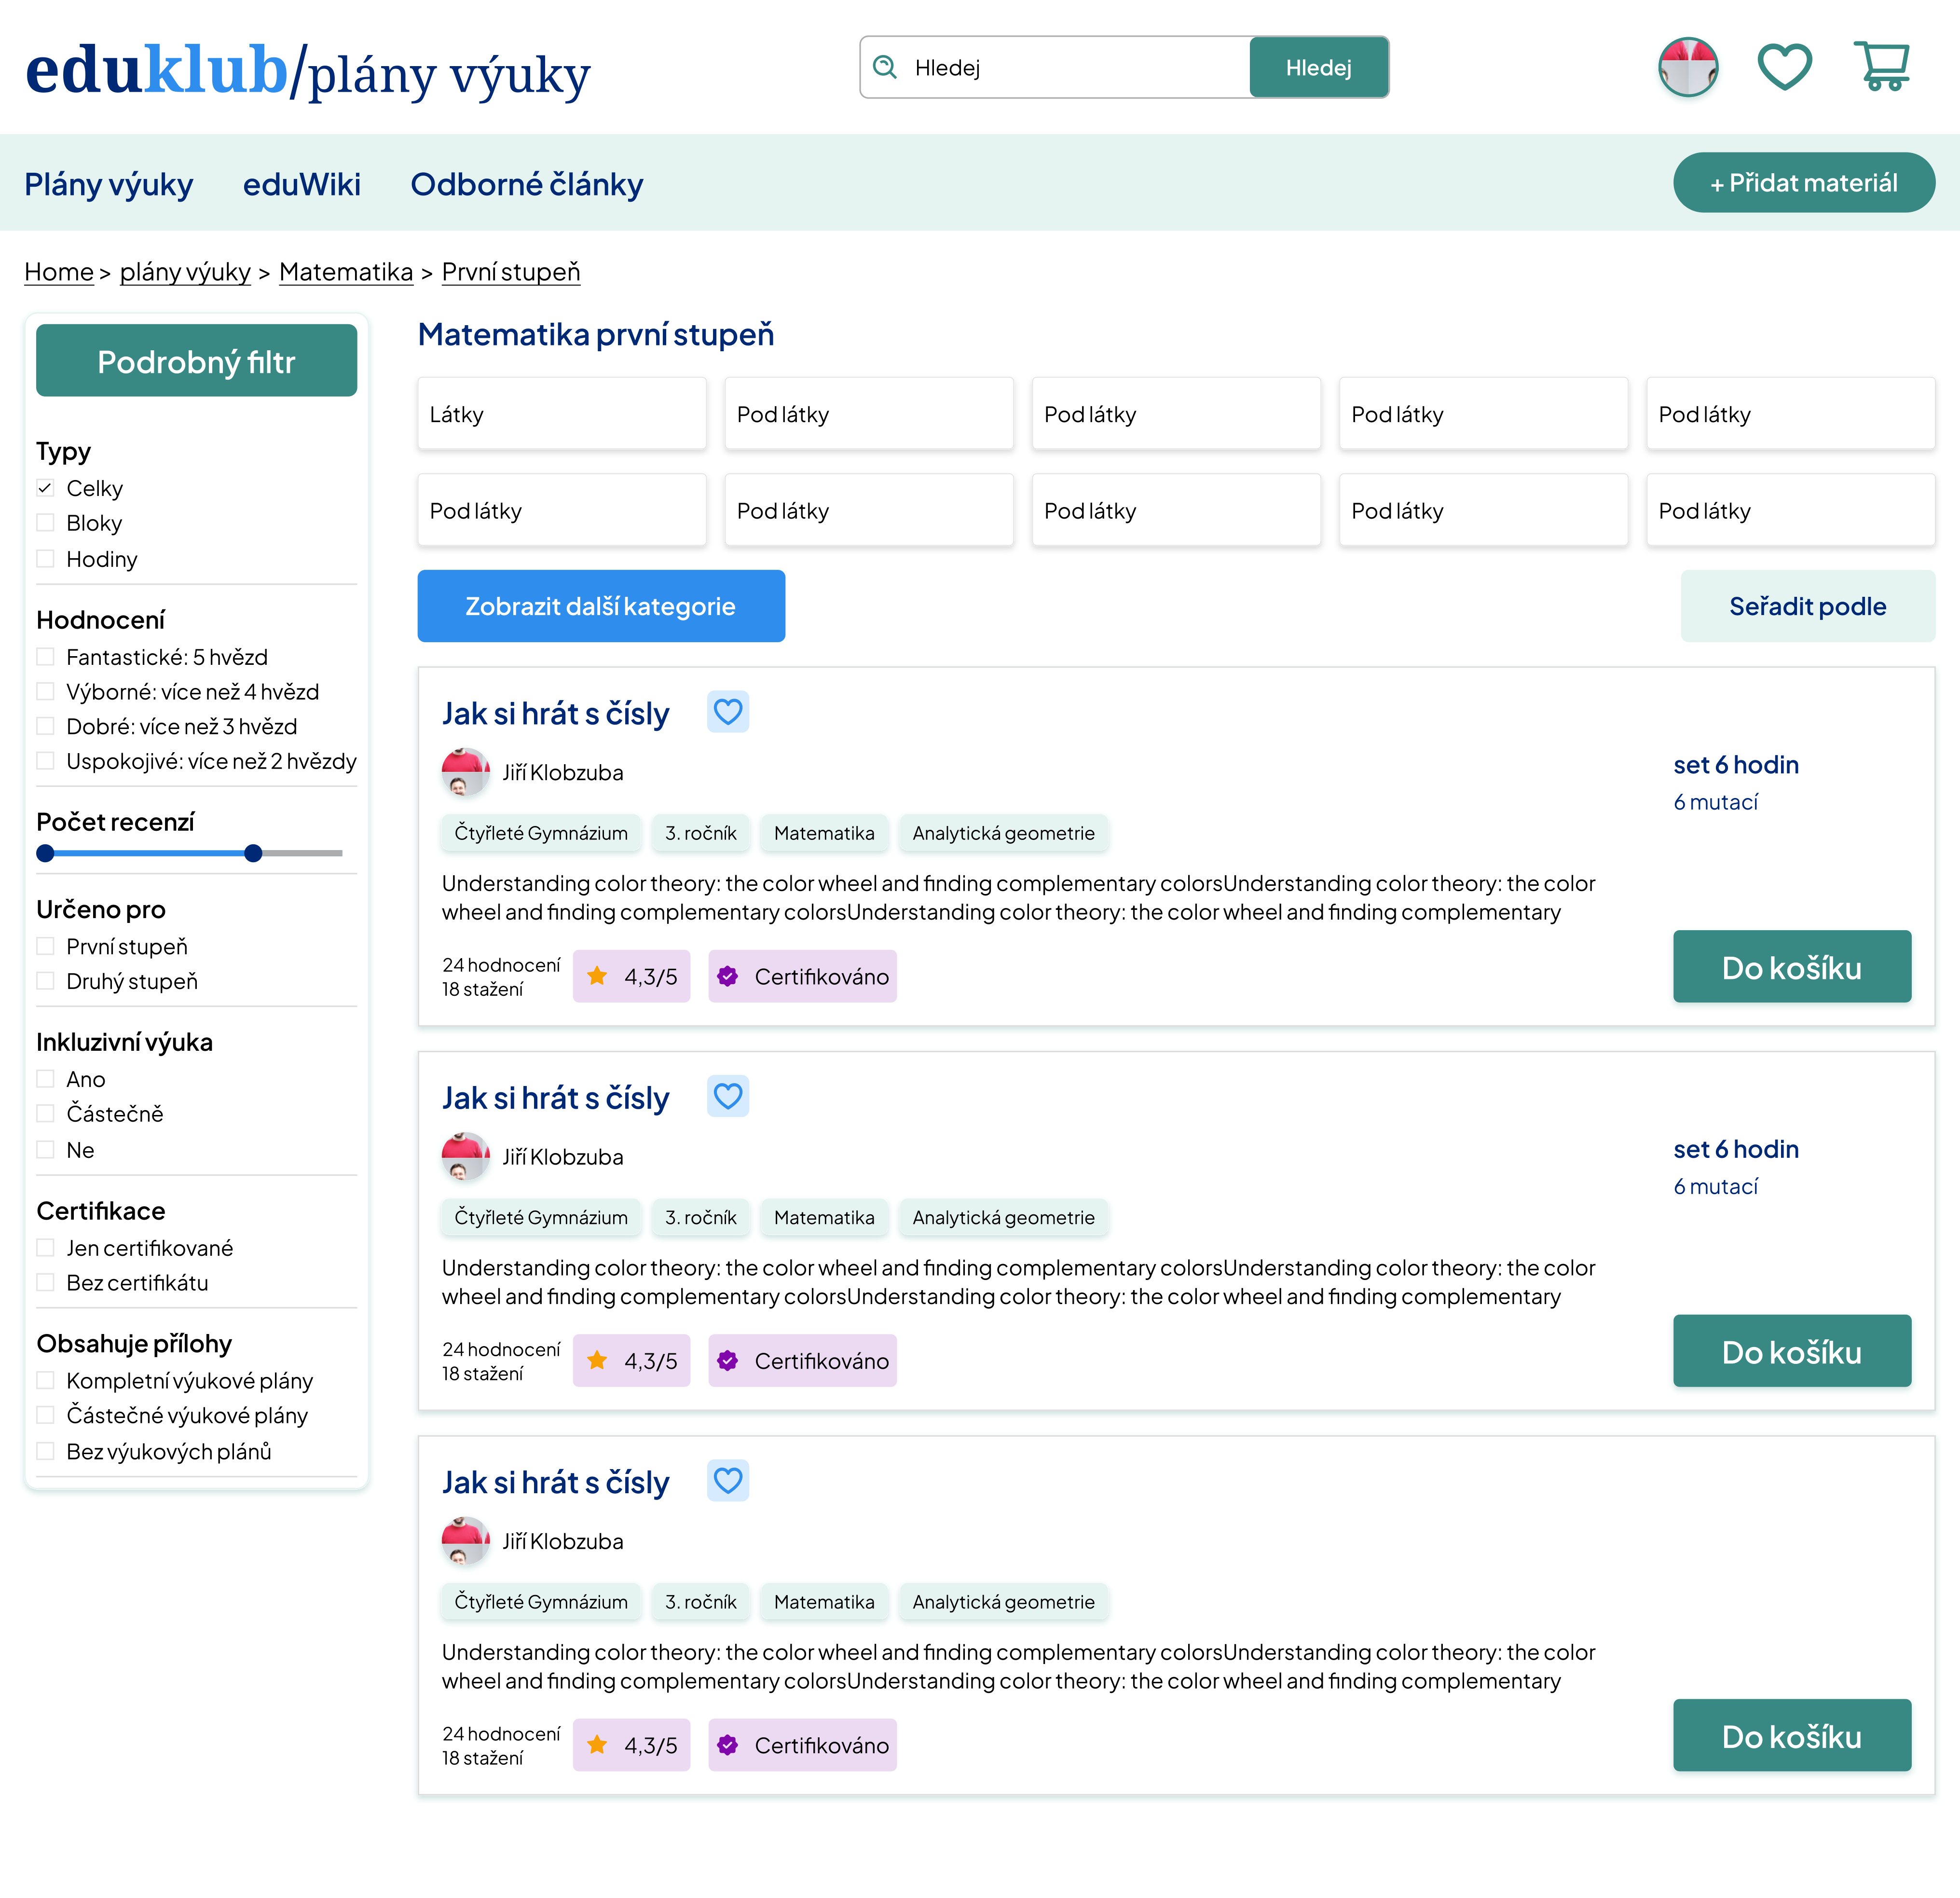
\includegraphics{eduklub-navrh-2.png}}
	\caption{Návrh uživatelského rozhraní vyhledávací stránky aplikace \textit{Eduklub~--~plány výuky}.}
	\label{fig:eduklub-navrh-2}
\end{figure}

\subsection{Domovská stránka webového agregátoru výukových plánů}

Domovská stránka webového agregátoru výukových plánů slouží jako hlavní rozcestník pro vyhledávání a~objevování výukových celků. Součástí stránky je vyhledávací pole, které umožňuje hledání podle klíčových slov a~usnadňuje orientaci mezi výukovými celky.

Pro zpřesnění hledání je k~dispozici několik filtrů, mezi které patří předmět, stupeň vzdělávání (1.~stupeň, 2.~stupeň, nižší gymnázium, vyšší gymnázium a~střední škola), ročník, jazyk, hodnocení (podle počtu hvězdiček 0--5) a~certifikace, která označuje výukové celky schválené pedagogy z~Univerzity Karlovy. Tyto filtry umožňují snadnější orientaci v~obsahu a~pomáhají uživatelům rychleji najít relevantní materiály.

\newpage

Pod vyhledávací sekcí se nachází oblast s~doporučenými výukovými celky. Administrátor má možnost ručně označit konkrétní výukový celek jako doporučený, čímž se zvyšuje jeho šance na~zobrazení na~domovské stránce. Tento systém umožňuje zdůraznit kvalitní materiály, které by mohly být pro uživatele nejvíce přínosné.

\begin{figure}[H]
	\centering
	\resizebox{16cm}{!}{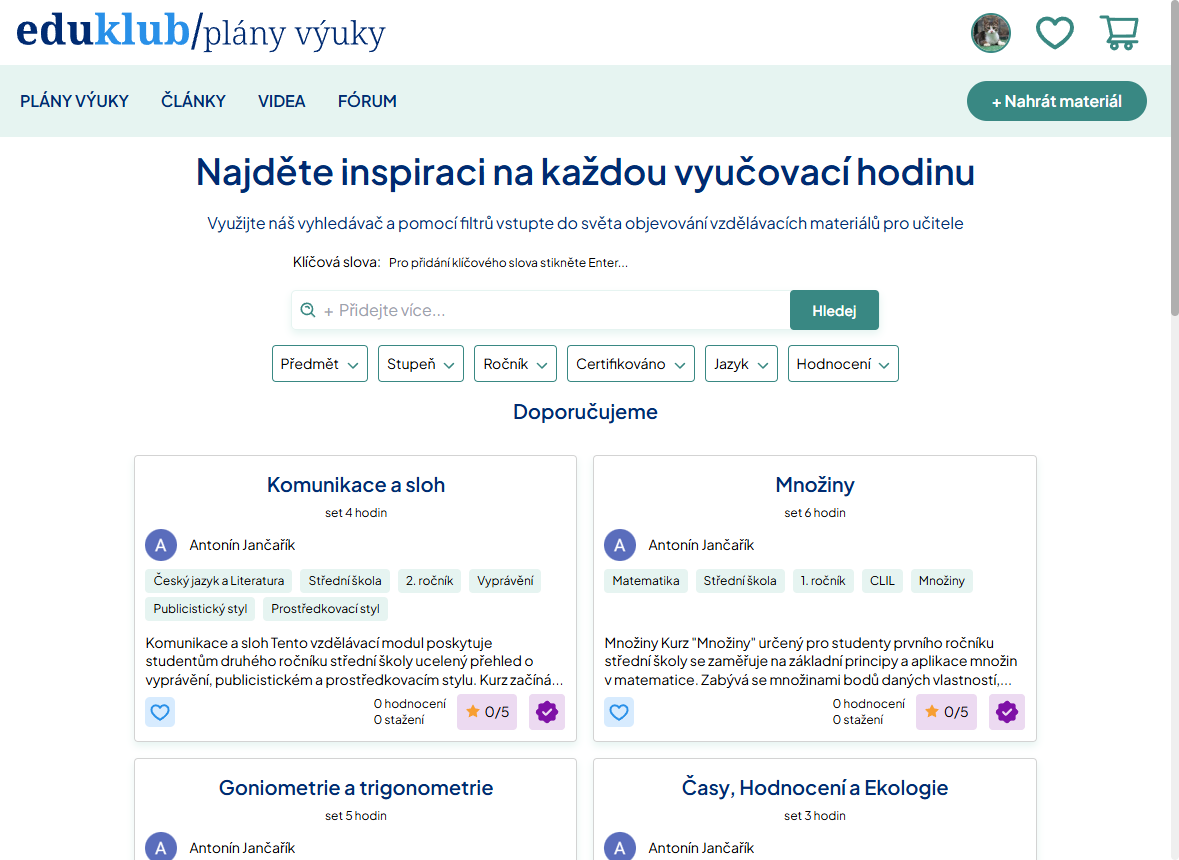
\includegraphics{eduklub-1.png}}
	\caption{Okno aplikace \textit{Eduklub~--~plány výuky} s~náhledem na~domovskou stránku.}
	\label{fig:eduklub-1}
\end{figure}

\subsection{Nahrání nového výukového plánu}

V~navigační liště se nachází tlačítko \quotedblbase Nahrát materiál``, které po~kliknutí otevře modální okno pro nahrání exportovaného výukového celku z~\textit{EDUBO}.

Po~výběru souboru je nutné zadat název a~popis, který lze upravovat pomocí WYSIWYG editoru. Předmět se automaticky nastaví podle názvu předmětu z~\textit{EDUBO}, ale lze jej upravit. Dále je třeba vybrat ročník, třídu, kategorii a~klíčová slova, která pomohou s~filtrováním obsahu. Uživatel má také možnost změnit jazyk výukového celku nebo přidat výstupy z~RVP, čímž zajistí přesnější zařazení materiálu do~vzdělávacího systému.

\begin{figure}[H]
	\centering
	\resizebox{13cm}{!}{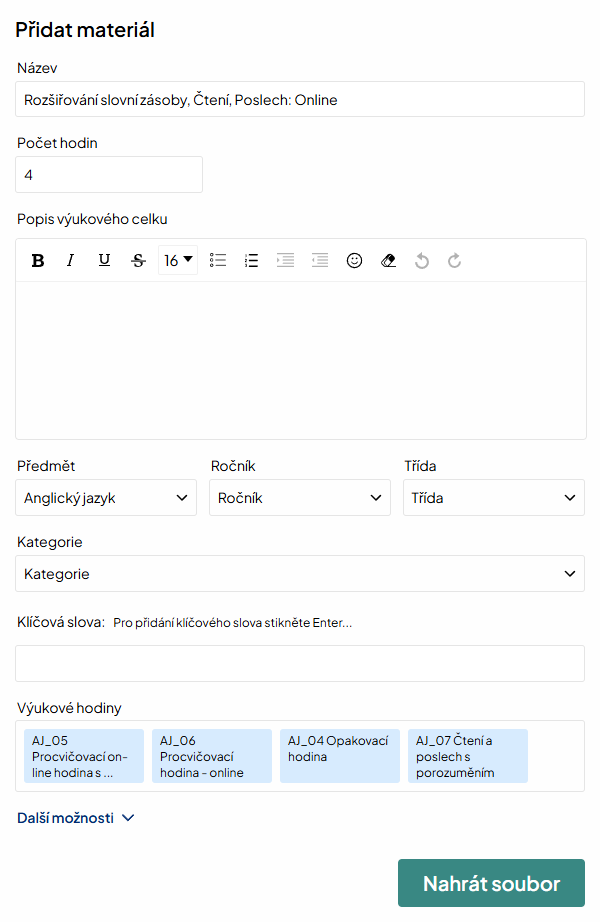
\includegraphics{eduklub-2.png}}
	\caption{Modální okno pro přidání nového výukového celku v~aplikaci\break\textit{Eduklub~--~plány výuky}.}
	\label{fig:eduklub-2}
\end{figure}

\newpage

\subsection{Vyhledávací stránka agregátoru výukových plánů}

Vyhledávací stránka poskytuje rozšířené možnosti filtrování a~umožňuje uživatelům najít výukové celky podle specifických kritérií. Kromě základních filtrů, které jsou dostupné i~na~domovské stránce, zde lze filtrovat výukové celky podle toho, zda se jedná o~mutace~--~tedy upravené verze existujících plánů.

Další možností je filtrování podle kategorií, které jsou přiřazeny ke~každému předmětu, což umožňuje přesnější vyhledávání. Výsledky lze také seřadit podle počtu stažení, hodnocení a~počtu výukových hodin, což usnadňuje nalezení nejpopulárnějších nebo nejlépe hodnocených výukových plánů.

\begin{figure}[H]
	\centering
	\resizebox{16cm}{!}{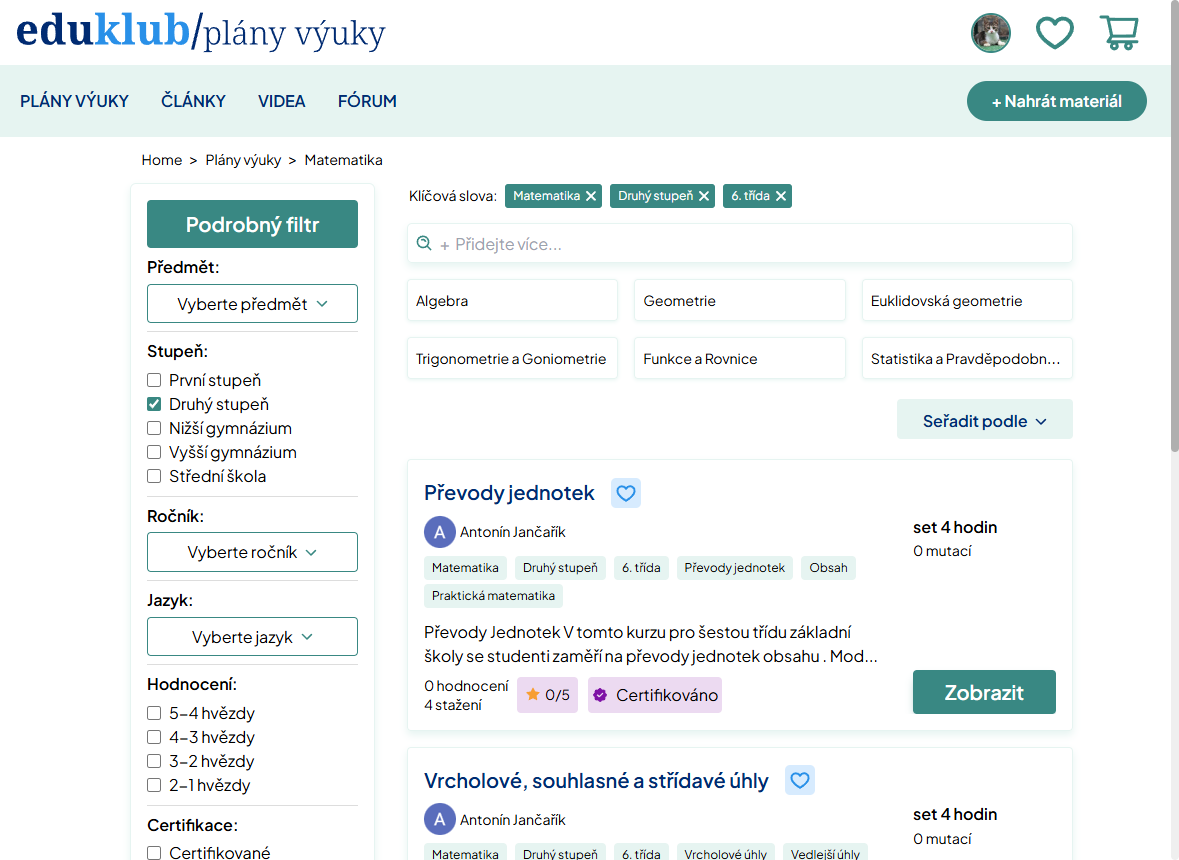
\includegraphics{eduklub-3.png}}
	\caption{Okno aplikace \textit{Eduklub~--~plány výuky} s~náhledem na~vyhledávací stránku.}
	\label{fig:eduklub-3}
\end{figure}

\begin{figure}[H]
	\centering
	\resizebox{16cm}{!}{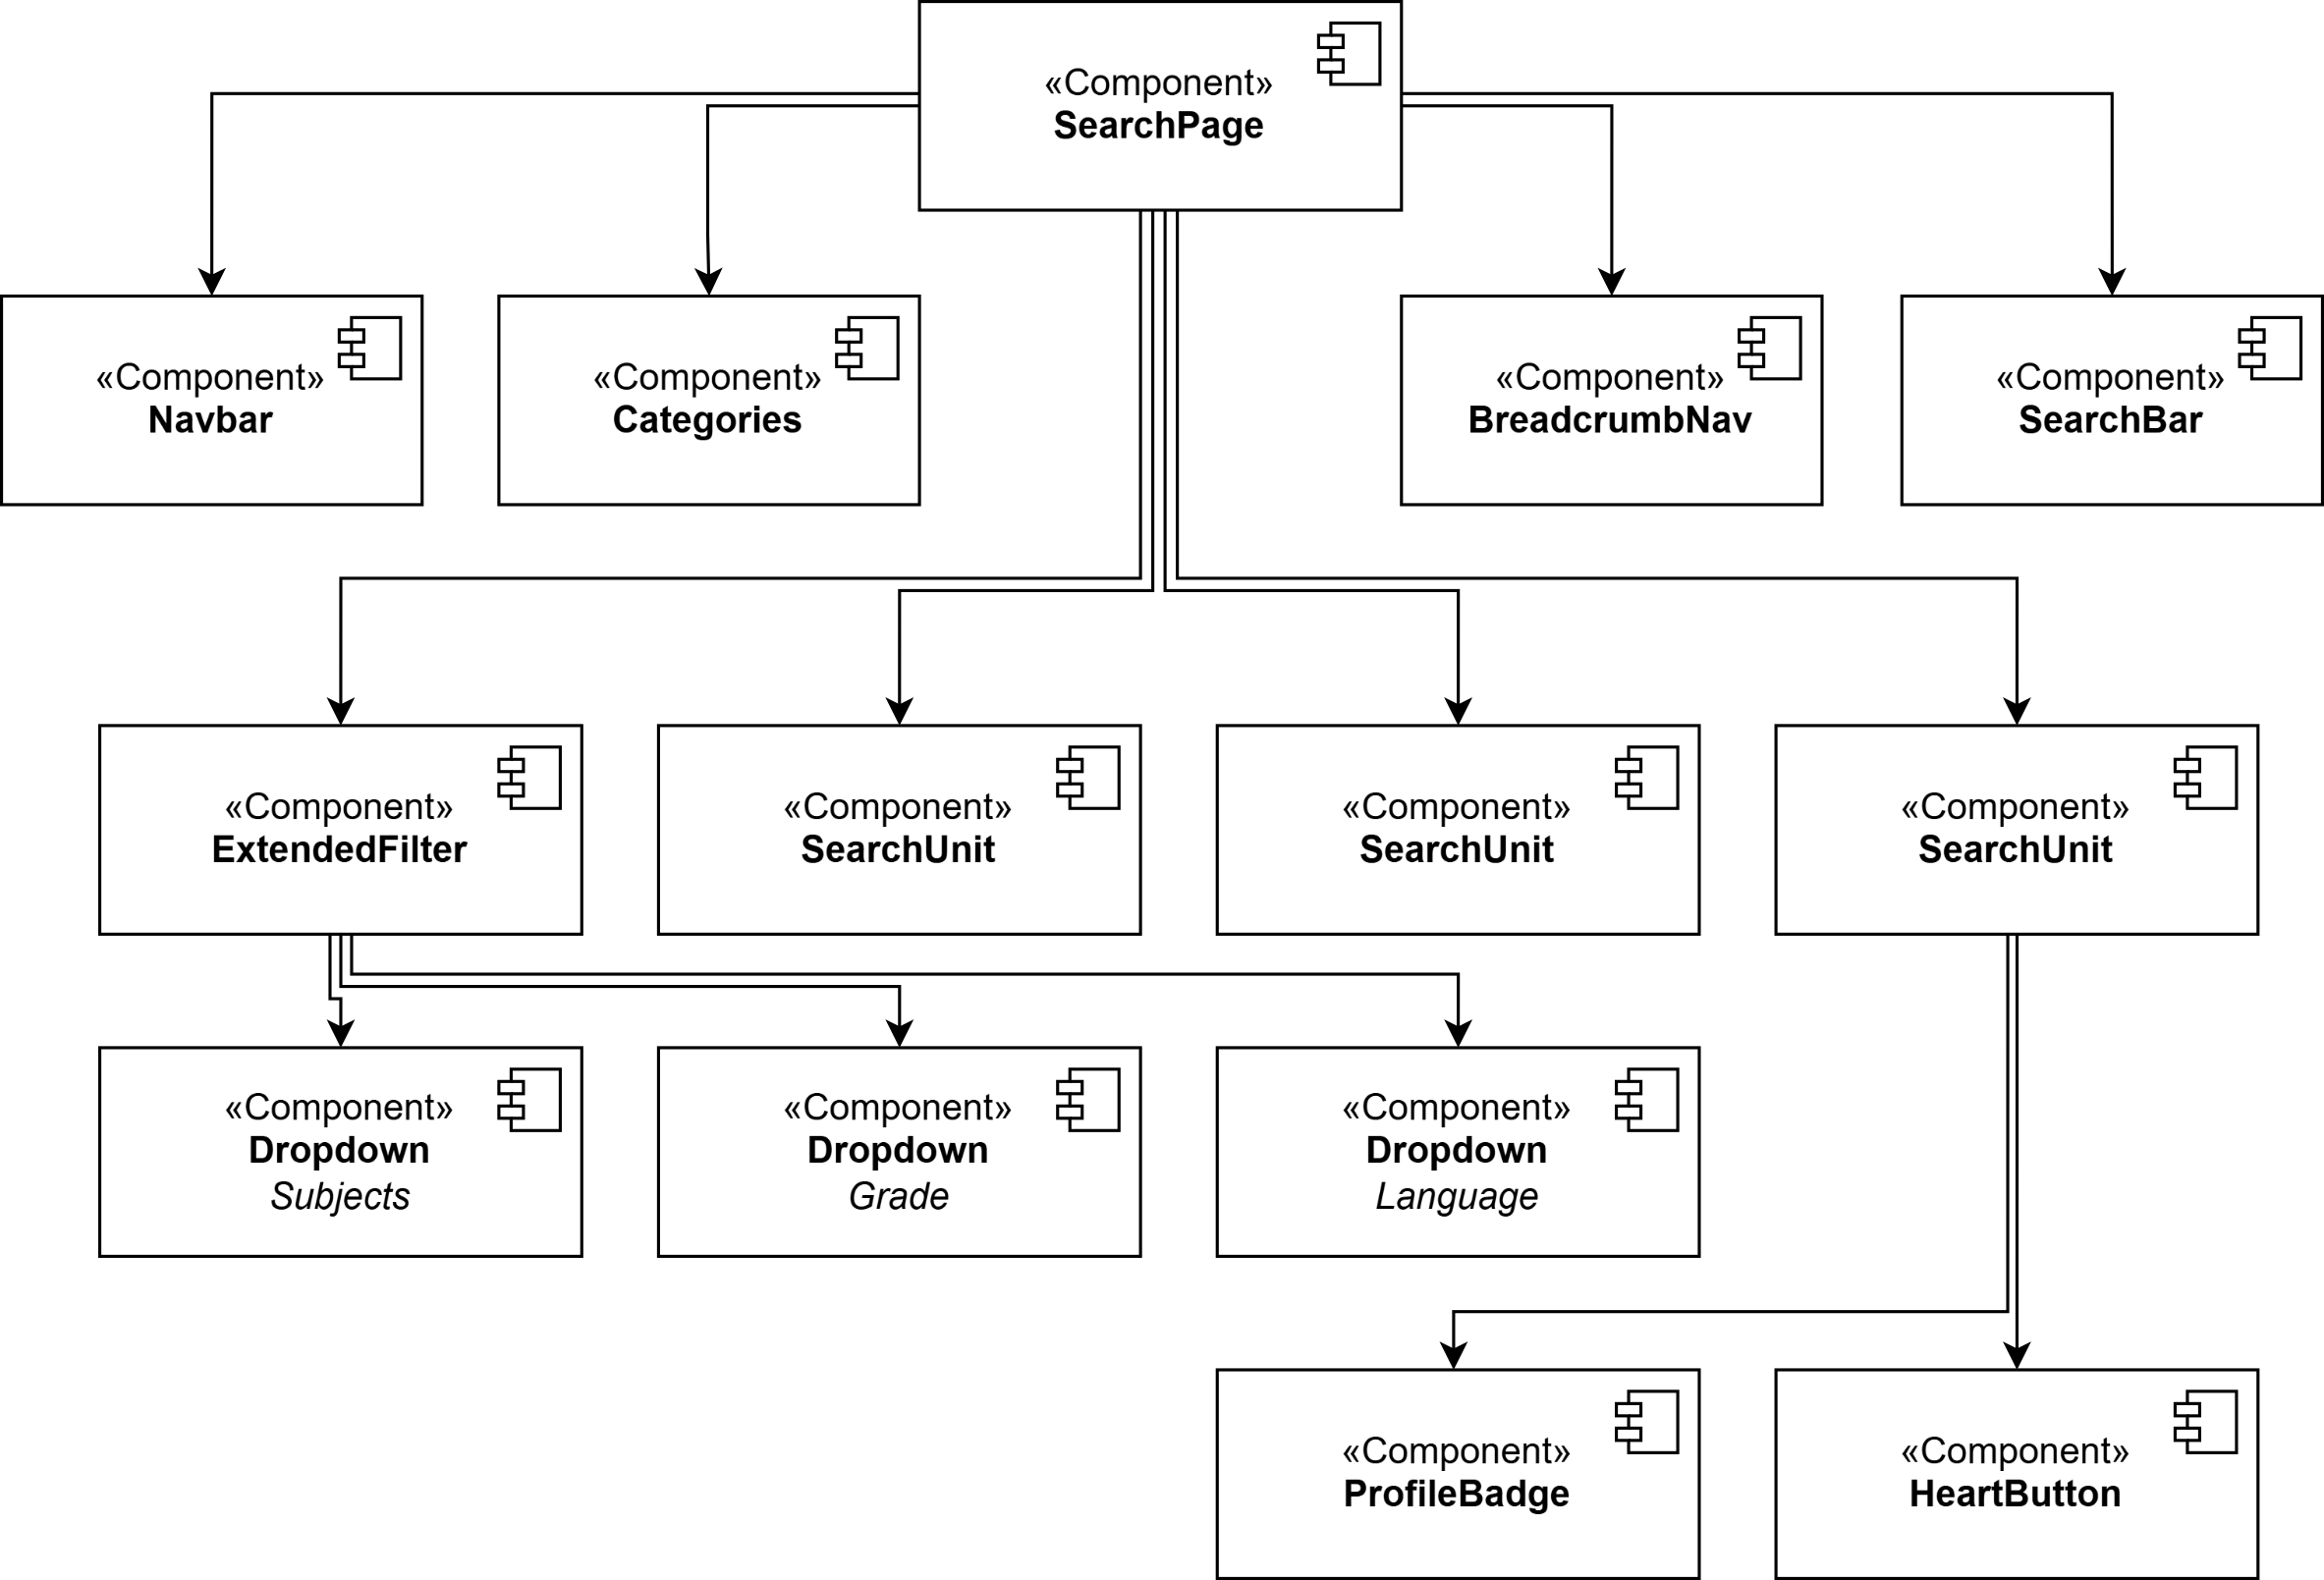
\includegraphics{component-diagram-react-3.png}}
	\caption{Komponentní diagram znázorňující strukturu React komponent na~vyhledávací stránce.}
	\label{fig:component-diagram-react-3}
\end{figure}

Tento komponentní diagram znázorňuje architekturu React komponent používaných na~stránce pro vyhledávání. Hlavní komponentou je \texttt{SearchPage}, která řídí zobrazování výsledků a~poskytuje přístup k~filtrům a~vyhledávání. Mezi klíčové komponenty patří \texttt{Navbar}, který slouží jako navigační lišta, \texttt{BreadcrumbNav}, jenž zobrazuje cestu mezi kategoriemi, a~\texttt{SearchBar}, který umožňuje hledání podle klíčových slov. Komponenta \texttt{Categories} umožňuje rychlý výběr z~předem definovaných kategorií.

Důležitou částí je komponenta \texttt{ExtendedFilter}, která nabízí pokročilé filtrování výukových plánů. Umožňuje uživatelům vybírat předměty, ročníky a~jazyky prostřednictvím rozbalovacích menu, reprezentovaných komponentami \texttt{Dropdown}. Samotné výsledky vyhledávání jsou reprezentovány komponentou \texttt{SearchUnit}, která zobrazuje jednotlivé výukové celky. Každá karta výukového plánu obsahuje komponentu \texttt{ProfileBadge}, jež zobrazuje informace o~autorovi a~\texttt{HeartButton}, který umožňuje přidat plán do~oblíbených.

% TODO: TADY ZMĚNIT KÓD JESTLI TO BUDE KÓD %
\begin{lstlisting}
export const getCachedCategories = async () => {
 const cachedObject = sessionStorage.getItem("categories");
 if (cachedObject) {
  const objects: TSubjectWithCategories[] = JSON.parse(cachedObject);
  if (objects) {
   return objects;
  }
 }

 const response = await axios.get("/api/categories/subjects");
 if (response.status === 404) {
  return [blankSubjectWithCategories];
 }
 const loadedObject: TSubjectWithCategories[] =
  response.data.sort((a:Category, b:Category) => a.id - b.id);

 sessionStorage.setItem("categories", JSON.stringify(loadedObject));
 if (loadedObject) {
  return loadedObject;
 }
 return [blankSubjectWithCategories];
};
\end{lstlisting}

Tato funkce \texttt{getCachedCategories} slouží k~efektivnímu načítání seznamu kategorií s~využitím mezipaměti (\texttt{sessionStorage}). Nejprve se pokusí načíst uložená data ze~\texttt{sessionStorage} pomocí klíče \texttt{categories}. Pokud jsou kategorie v~mezipaměti, převedou se zpět na~objekt a~ihned se vrátí, čímž se šetří volání na~server.

Pokud kategorie v~mezipaměti nejsou, provede se asynchronní požadavek na~backend. V~případě chyby \texttt{404} se vrátí výchozí prázdný objekt \texttt{blankSubjectWithCategories}. Jinak se získaná data seřadí podle \texttt{id} a~uloží do~\texttt{sessionStorage}, aby se při dalším volání funkce nemusel znovu kontaktovat backend. Poté se vrátí načtený a~uložený seznam kategorií.

\subsubsection{Stránka náhledu výukového celku}

Stránka náhledu výukového celku poskytuje podrobný přehled o~konkrétním výukovém celku a~jeho obsahu. Uživatel zde vidí základní informace, jako je název plánu, autor, klíčová slova a~další metadata. Struktura stránky je rozdělena do~několika záložek, které umožňují přístup k~různým detailům výukového celku.

Záložka \textbf{Popis} obsahuje textový přehled výukového plánu. Náhled plánu umožňuje prohlédnout PDF exporty všech výukových hodin, které výukový celek obsahuje. Sekce \textbf{Hodnocení} umožňuje uživatelům hodnotit výukový celek pomocí hvězdičkového systému (0--5 hvězdiček) a~přidávat plusy a~mínusy. \textbf{Výstupy RVP} zobrazují všechny kurikulární výstupy rámcového vzdělávacího programu, které jsou v~celku zahrnuty. Záložka \textbf{Poradna a~návody} obsahuje odkazy na~články v~Eduklubu, které mohou být užitečné pro danou výuku. V~sekci \textbf{Alternativy} může autor přidat výukové plány, které jsou tematicky podobné. V~sekci \textbf{Mutace} se zobrazují upravené varianty původního výukového plánu.

\begin{figure}[H]
	\centering
	\resizebox{16cm}{!}{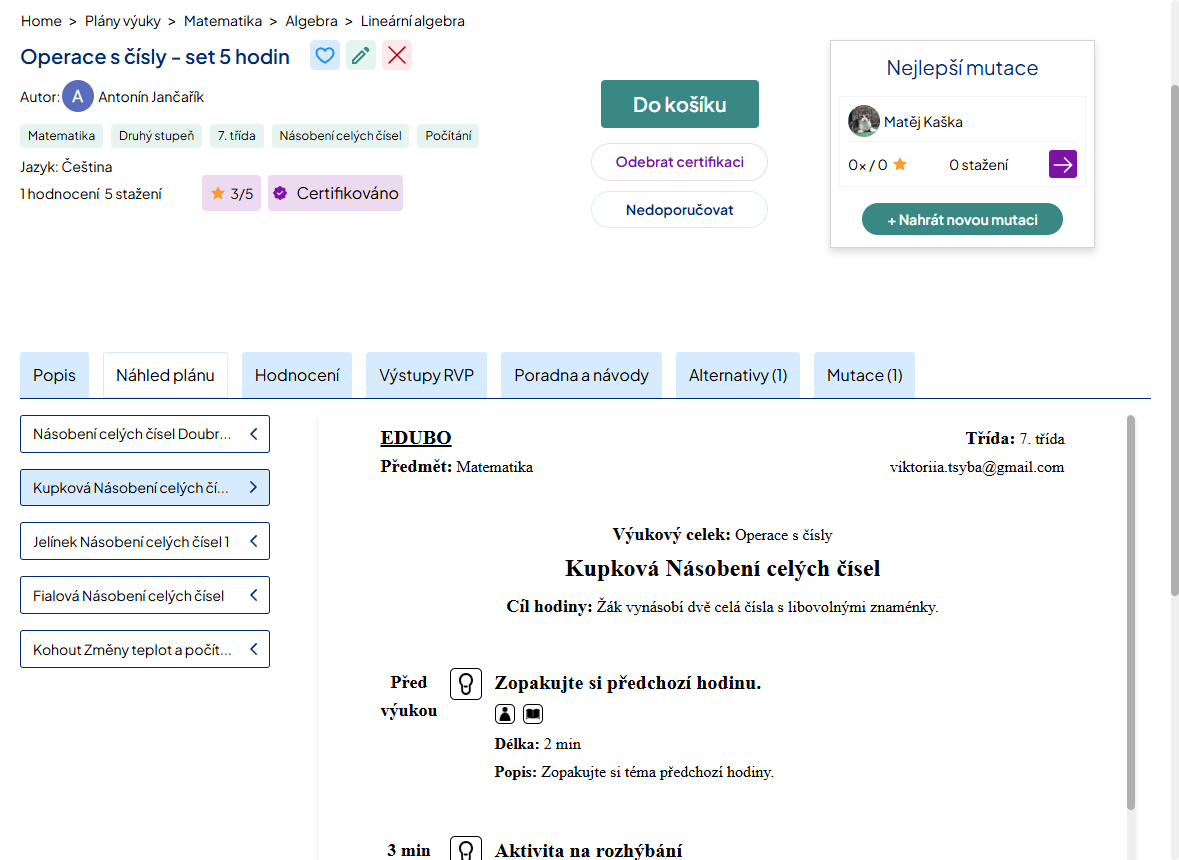
\includegraphics{eduklub-4.png}}
	\caption{Okno aplikace \textit{Eduklub~--~plány výuky} s~náhledem na~stránku náhledu výukového celku.}
	\label{fig:eduklub-4}
\end{figure}

\section{Uživatelský manuál}

V~této kapitole si představíme dva základní scénáře práce s~aplikací \textit{EDUBO} z~pohledu učitele a~žáka. Nejprve si krok za~krokem ukážeme proces registrace učitele, vytvoření třídy, předmětu, výukového celku, výukového plánu a~publikace výukové hodiny. Následně se zaměříme na~to, jak se do~systému přihlašuje žák, jaké prostředí ho po~přihlášení čeká a~jakým způsobem se dostane ke~své výukové hodině. Každý krok je podrobně popsán, aby byl snadno srozumitelný i~pro uživatele, kteří s~aplikací začínají.

\subsection{1.~scénář:~Prvotní registrace učitele, vytvoření výukového plánu a~vytvoření přístupových klíčů pro žáky}

\subsubsection{Krok~1:~Registrace učitele}
Aplikaci \textit{EDUBO} můžete otevřít v~testovacím prostředí na~adrese \url{https://app.eduklub.cz/}. Na~úvodní obrazovce \textit{EDUBO} klikněte na~tlačítko \quotedblbase Registrovat se``, které vás přesměruje na~registrační formulář. Zde vyplňte svůj e-mail, heslo a~registrační klíč. Tento klíč určuje vaše školní zařízení a~je poskytován školou. Na~testovacím nasazení je klíč \quotedblbase teacher``. Zaškrtněte souhlas se~zpracováním osobních údajů. Po~registraci se přihlaste do~\textit{EDUBO} se~svými novými přihlašovacími údaji.

\subsubsection{Krok~2:~Vytvoření třídy}
Po~přihlášení je potřeba vytvořit třídu, do~které budete přidávat žáky. Klikněte na~ikonu \quotedblbase plus`` v~sekci Třídy. Zde máte možnost buď přidat se do~již existující třídy nebo vytvořit třídu novou. Zadejte název třídy a~klikněte na~tlačítko pro vytvoření.

\subsubsection{Krok~3:~Vytvoření předmětu}
Po~vytvoření třídy přejděte na~sekci \quotedblbase Předměty``, kde klikněte na~tlačítko \quotedblbase plus``. Zadejte název předmětu, který bude v~rámci třídy vyučován. Můžete také přiřadit kurikulární výstupy kliknutím na~tlačítko \quotedblbase Přiřadit výstupy k~předmětu``, vyberte požadované kurikulární výstupy a~přiřaďte je k~předmětu.

\begin{figure}[H]
	\centering
	\resizebox{12cm}{!}{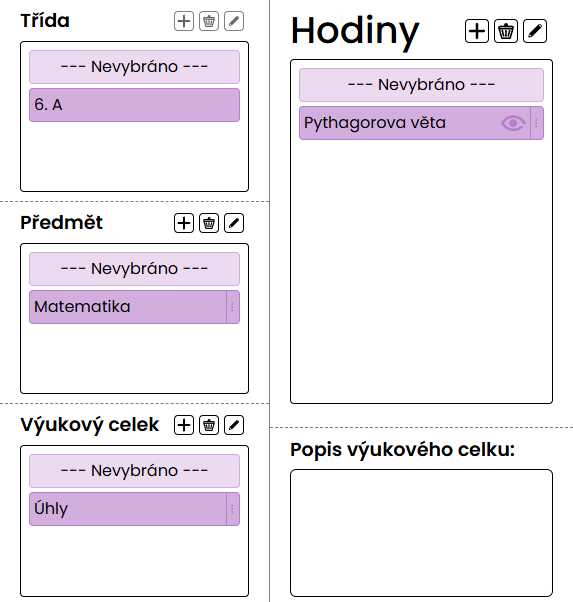
\includegraphics{manual-1.png}}
	\caption{Část uživatelského menu aplikace \textit{EDUBO}.}
	\label{fig:manual-1}
\end{figure}

\subsubsection{Krok~4:~Vytvoření výukového celku}
Následně vytvořte výukový celek kliknutím na~tlačítko \quotedblbase plus`` v~sekci \quotedblbase Výukové celky``. Zadejte název výukového celku a~potvrďte jeho vytvoření.

\subsubsection{Krok~5:~Vytvoření výukového plánu}
Nyní přejděte do~sekce \quotedblbase Hodiny`` a~klikněte na~tlačítko \quotedblbase plus`` pro vytvoření výukového plánu. Zadejte název plánu a~klikněte na~\quotedblbase Vytvořit``. V~pravém dolním rohu menu klikněte na~tlačítko \quotedblbase Editovat``, které vás přesměruje do~editoru výukového plánu.

\subsubsection{Krok~6:~Editace výukového plánu}
V~editoru výukového plánu můžete v~horní části změnit název, přidat cíl hodiny a~přiřadit kurikulární výstupy. V~pravém dolním rohu se nachází textové pole pro poznámky. V~levém sloupci můžete vybírat mezi různými typy aktivit a~přetáhnout je na~plátno pomocí drag and drop\break interakce. Pokud nevíte, jak využít konkrétní aktivitu, klikněte na~informační tlačítko u~dané aktivity, které otevře podrobné metodické materiály s~návody na~jejich efektivní využití ve~výuce.

Každou aktivitu můžete upravit kliknutím na~tlačítko tužky u~konkrétní aktivity. Zde můžete měnit název, popis, délku, pomůcky, soubory, odkazy, organizační formu a~formu činnosti.

\begin{figure}[H]
	\centering
	\resizebox{12cm}{!}{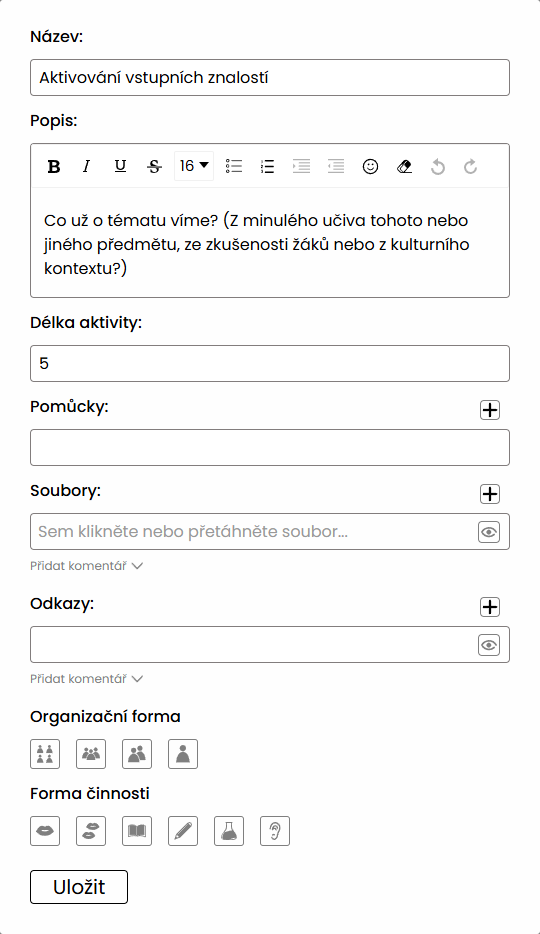
\includegraphics{manual-2.png}}
	\caption{Modální okno pro~úpravu aktivity v~aplikaci \textit{EDUBO}.}
	\label{fig:manual-2}
\end{figure}

\newpage

\subsubsection{Krok~7:~Uložení výukového plánu}
Po~vytvoření výukového plánu a~přidání všech aktivit, uložte svůj výukový plán pomocí navigační lišty: \textit{Soubor}~$\rightarrow$~\textit{Uložit výukovou hodinu}. Poté se vraťte zpět do~menu: \textit{Soubor}~$\rightarrow$~\textit{Zpět do menu}.

\begin{figure}[H]
	\centering
	\resizebox{8cm}{!}{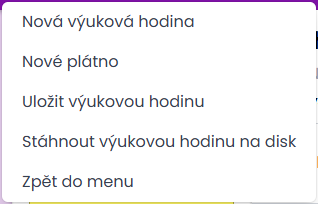
\includegraphics{manual-3.png}}
	\caption{Rozbalovací nabídka tlačítka \quotedblbase Soubor`` v~navigační liště v~aplikaci \textit{EDUBO}.}
	\label{fig:manual-3}
\end{figure}

\subsubsection{Krok 8:~Publikace výukového plánu}
Vyberte právě vytvořený výukový plán, nastavte datum a~čas konání hodiny v~pravém dolním rohu a~klikněte na~tlačítko \quotedblbase Publikovat``, aby byla hodina zveřejněna pro žáky.

\begin{figure}[H]
	\centering
	\resizebox{8cm}{!}{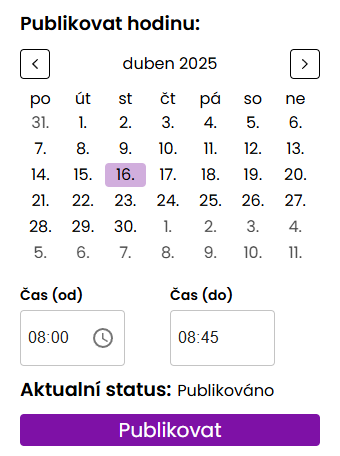
\includegraphics{manual-4.png}}
	\caption{Část uživatelského menu určeného pro~publikování výukového plánu v~aplikaci \textit{EDUBO}.}
	\label{fig:manual-4}
\end{figure}

\newpage

\subsubsection{Krok~9:~Generování registračních klíčů pro žáky}
Pro~vytvoření registračních klíčů pro~žáky vyberte svou třídu a~v~navigační liště klikněte na~tlačítko \quotedblbase Generovat klíče``. Zadejte požadovaný počet klíčů, které chcete vygenerovat. Po~zadání počtu se vygenerují klíče, které si můžete vytisknout a~předat žákům.

\begin{figure}[H]
	\centering
	\resizebox{12cm}{!}{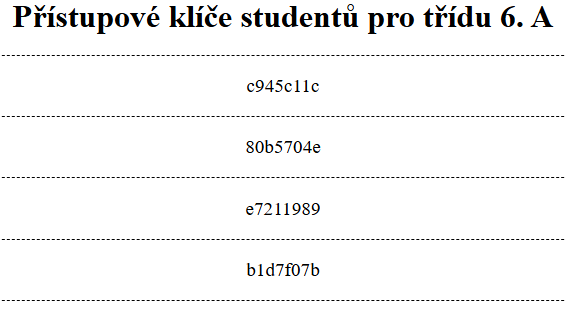
\includegraphics{manual-5.png}}
	\caption{Ukázka vygenerovaných přístupových klíčů studentů pro~třídu 6.~A připravených k~tisku.}
	\label{fig:manual-5}
\end{figure}

\subsection{2.~scénář:~Prvotní registrace žáka, zobrazení pohledů a~zobrazení výukové hodiny}

\subsubsection{Krok~1:~Registrace žáka}
Aplikaci \textit{EDUBO} můžete otevřít v~testovacím prostředí na~adrese \url{https://app.eduklub.cz/}. Na~úvodní obrazovce klikněte na~tlačítko \quotedblbase Registrovat se``, které vás přesměruje na~registrační formulář. Zadejte svůj e-mail, zvolte heslo a~vložte registrační klíč, který vám předal učitel. Na~testovacím nasazení si můžete klíč vygenerovat sami (viz~1.~scénář, krok~9). Nezapomeňte zaškrtnout souhlas se~zpracováním osobních údajů. Po~dokončení registrace se přihlaste do~\textit{EDUBO} pomocí zadaných údajů.

\newpage

\subsubsection{Krok~2:~Výběr pohledu}
Po~přihlášení si žák volí mezi dvěma pohledy~--~\textbf{Předměty} a~\textbf{Kalendář}.

\begin{figure}[H]
	\centering
	\resizebox{6cm}{!}{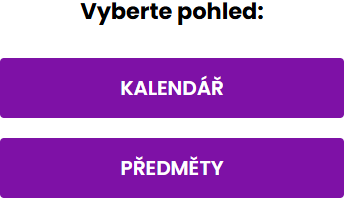
\includegraphics{manual-6.png}}
	\caption{Rozhraní pro výběr pohledu ve studentském menu.}
	\label{fig:manual-6}
\end{figure}

\subsubsection{Pohled Předměty}
Pohled Předměty nabízí přehled všech předmětů vyučovaných ve~třídě. Po~kliknutí na~konkrétní předmět se zobrazí výukové celky, a~následně i~publikované hodiny. V~dolní části obrazovky žák najde materiály k~hodině~--~přílohy, odkazy, pomůcky a~možnost hodnocení pomocí smajlíků. Vpravo jsou zobrazeny informace o~hodině.

\begin{figure}[H]
	\centering
	\resizebox{6cm}{!}{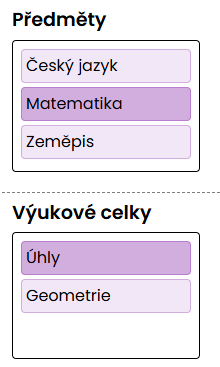
\includegraphics{manual-7.png}}
	\caption{Navigace předmětů a~výukových celků v~pohledu předměty.}
	\label{fig:manual-7}
\end{figure}

\begin{figure}[H]
	\centering
	\resizebox{14cm}{!}{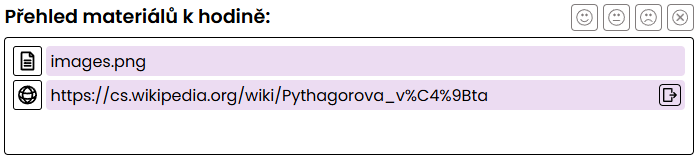
\includegraphics{manual-8.png}}
	\caption{Rozhraní přehledu materiálů ve~vybraném výukovém plánu.}
	\label{fig:manual-8}
\end{figure}

\subsubsection{Pohled Kalendář}
Pohled Kalendář zobrazuje v~levé části měsíční kalendář. Po~výběru konkrétního dne se ve~střední části zobrazí zkrácený přehled hodin publikovaných v~daný den. Ten připomíná PDF export hodiny. I~zde je ve~spodní části seznam všech materiálů a~v~pravé části podrobný popis hodiny.

\begin{figure}[H]
	\centering
	\resizebox{8cm}{!}{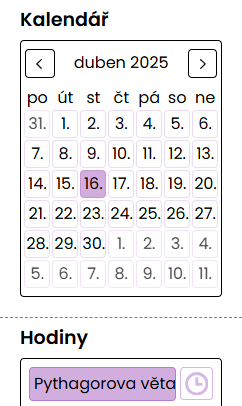
\includegraphics{manual-9.png}}
	\caption{Navigace hodin a~kalendář v~pohledu kalendář.}
	\label{fig:manual-9}
\end{figure}

\begin{figure}[H]
	\centering
	\resizebox{14cm}{!}{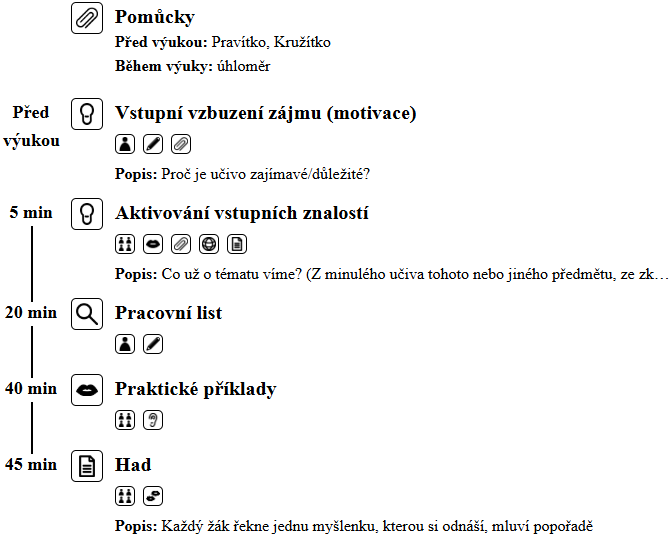
\includegraphics{manual-10.png}}
	\caption{Zkrácený přehled výukového plánu v~pohledu kalendář.}
	\label{fig:manual-10}
\end{figure}

\subsubsection{Krok~3:~Zobrazení výukového plánu}
Pomocí tlačítka \quotedblbase Otevřít`` vpravo dole se žák dostane k~podrobné struktuře výukového plánu. Zde si může zobrazit samotné plátno s~aktivitami~--~každá aktivita se dá rozkliknout a~zobrazí se její popis, délka, potřebné pomůcky, odkazy či přiložené soubory.

\begin{figure}[H]
	\centering
	\resizebox{14cm}{!}{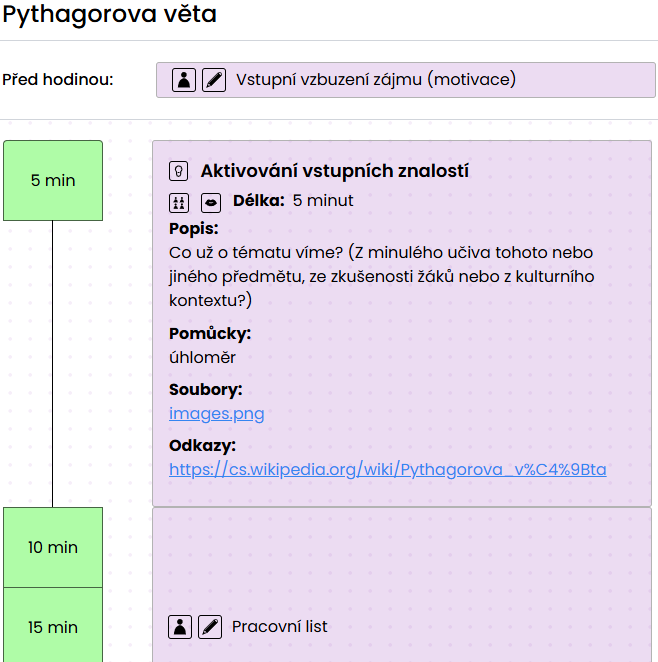
\includegraphics{manual-11.png}}
	\caption{Zobrazení výukového plánu ve~studentském rozhraní.}
	\label{fig:manual-11}
\end{figure}


\chapter{Testování softwaru uživateli}

Aplikace \textit{EDUBO} byla testována průběžně během celého vývoje. V~počáteční fázi jsme testovali aplikaci interně. Zaměřovali jsme se na~ověření základní funkčnosti jako registrace, přihlašování, vytváření výukových plánů a~přetahování aktivit v~plátně. První iterace sloužila především k~technickému ověření základních scénářů a~stabilitě editoru.

Od~druhé iterace jsme začali zapojovat skutečné uživatele~--~pedagogy z~Pedagogické fakulty Univerzity Karlovy, kteří začali v~\textit{EDUBO} vytvářet své výukové plány, které se později publikovali na~webu \textit{Eduklub~--~plány výuky}. Tím se ukázala silná stránka nástroje jako podpory pro reálnou pedagogickou činnost, ale současně vyvstala i~řada nedostatků. Mezi nejvýznamnější patřilo špatné vykreslování názvu výukového plánu~--~při delším názvu nebyl text zcela viditelný, dále padání aplikace při vkládání rovnic z~Microsoft Word nebo nemožnost posouvat modální okno při úpravě aktivity na~touchpadech gestem. Všechny tyto chyby byly postupně identifikovány, zaznamenány a~odstraněny.

V~roce 2024 se \textit{EDUBO} stalo nástrojem i~pro výuku studentů Pedagogické fakulty Univerzity J.~E.~Purkyně. Přibližně 250 studentů mělo za~úkol vytvořit vlastní výukový plán. Jejich zpětná vazba byla velmi cenná~--~většina z~nich hodnotila aplikaci pozitivně, chválili intuitivní ovládání, přehlednost a~celkový přínos při strukturování hodiny. Objevila se však také závažná technická chyba: pokud uživatel přetáhl aktivitu do~plátna a~v~rychlém sledu chytil jinou, aplikace spadla. Jednalo se o~problém v~knihovně \texttt{react-beautiful-dnd}, která zajišťuje přetahování prvků a~od~roku 2022 nebyla aktualizována. Vzhledem k~tomu bylo nutné implementovat vlastní řešení~--~uživatel může nyní pracovat vždy pouze s~jednou aktivitou najednou, čímž se problém eliminoval. Potěšující bylo, že i~po~skončení kurzu někteří studenti pokračovali v~používání \textit{EDUBO} a~kontaktovali mě s~dotazy ohledně dalšího vývoje aplikace, což potvrzuje její využitelnost i~v~praxi.

V~roce 2025 proběhla rozsáhlá technická revize kódu. Došlo k~aktualizaci používaných balíčků, refaktoringu struktury aplikace, opravě mnoha drobných stylových chyb a~přidání nových animací. Zároveň došlo k~významnému zrychlení načítání aplikace~--~velikost přenášených dat se snížila z~původních 8~MB na~0{,}8~MB, což se pozitivně projevilo na~výkonu i~použitelnosti aplikace při slabším připojení.

Na~rozdíl od~\textit{EDUBO} nebyla aplikace \textit{Eduklub~--~plány výuky} zatím reálně otestována cílovými uživateli. Ačkoli je její technická příprava dokončena, čeká se na~rozhodnutí o~dalším směřování projektu. Věříme však, že i~tato platforma má potenciál stát se užitečným nástrojem pro sdílení inspirativních výukových plánů mezi pedagogy.

Celkově lze říci, že \textit{EDUBO} se díky intenzivní zpětné vazbě a~opakovanému testování v~reálném provozu stalo stabilním a~prakticky využívaným nástrojem. Zkušenosti učitelů i~studentů se výrazně promítly do~vývoje a~pomohly aplikaci přiblížit jejím uživatelům.


\chapter{Diskuse a výsledky}

Vývoj softwaru \textit{EDUBO} byl technicky i~organizačně náročným, ale zároveň velmi přínosným procesem. V~rámci hlavního vývoje bylo do~repozitáře \textit{EDUBO} odevzdáno přes 1500 commitů (příspěvků kódu), přičemž hlavní vývoj trval 11~měsíců. Následná fáze údržby pokračuje dodnes, kdy jsou prováděny menší opravy, aktualizace a~úpravy dle zpětné vazby uživatelů. V~případě doplňkové aplikace \textit{Eduklub~--~plány výuky} šlo o~více než 600~commitů a~vývoj trval přibližně čtyři měsíce, přičemž také tato část je i~nadále udržována.

Technologicky šlo o~náročný projekt, jehož největší výzvou byl bezesporu vlastní \textit{drag and drop} editor výukových plánů. Právě jeho vývoj byl velmi náročný zejména kvůli původnímu rozhodnutí použít knihovnu, která se již dlouho neudržovala a~obsahovala množství chyb. To vedlo ke~komplikacím, které se musely řešit implementací oprav, čímž se zvýšila udržitelnost a~stabilita této klíčové části systému.

Aplikace \textit{EDUBO} je v~současnosti nasazena na~serverech společnosti Mironet.cz a.s., kde funguje stabilně a~je dostupná pro každého, kdo si ji chce vyzkoušet. Ve~fázi testování byla aplikace využívána pedagogy Pedagogické fakulty Univerzity Karlovy, kteří v~ní vytvořili přes 200~výukových plánů a~studenty Pedagogické fakulty Univerzity Jana Evangelisty Purkyně, kteří v~ní vytvořili přes 250~výukových plánů. Přestože v~tuto chvíli není aplikace využívána plošně, základ je připraven a~existuje potenciál pro širší nasazení.

V~rámci vývoje se ukázalo několik oblastí, které by bylo vhodné dále rozpracovat. Hlavní prioritou je přepsání backendu \textit{EDUBO} z~Flasku na~Django a~přechod z~databáze MongoDB na~PostgreSQL, což by do~budoucna výrazně zjednodušilo údržbu i~rozšiřování systému. Mezi další rozvojové oblasti patří například vytvoření správy tříd a~jejich organizace, vytvoření jednoduššího instalačního skriptu pro nasazení vlastních verzí \textit{EDUBO} a~vylepšení UI/UX studentského pohledu, aby byl pro žáky přehlednější a~atraktivnější.

\chapter{Závěr}

Vytvoření softwaru \textit{EDUBO} pro mě představovalo zásadní milník~--~nejen po~technické, ale i~osobní stránce. Šlo o~první velký projekt, který jsem vedl jako leader týmu a~který měl zároveň dopad na~vzdělávání. Ačkoliv jsem původně do~projektu vstupoval jako programátor, postupně jsem převzal i~zodpovědnost za~organizaci celého vývoje, komunikaci s~týmem a~pedagogickými pracovníky a~koordinaci jednotlivých etap práce.

V~této roli jsem získal zkušenosti, které bych jinde získával mnohem déle. Musel jsem vést pravidelné stand-upy, řešit krizové situace, ale zároveň i~pomáhat méně zkušeným kolegům a~přispívat k~učení v~týmu. Například na~konci první iterace, kdy se spojoval frontend s~backendem a~došlo ke~kolapsu funkcionalit, jsem trávil celé dny opravami a~uvědomil si, že bez lepší metodiky a~kontroly nelze takto velký projekt efektivně řídit. I~proto jsem se ujal vedení vývoje a~nastavoval standardy, které do~té doby chyběly.

Nejvíce mě naplňovala kombinace samotného programování a~podpory ostatních. Měl jsem možnost se učit nové technologie jako React a~Django od~kolegů a~zároveň předávat své zkušenosti dál. Díky tomu se rozvinulo nejen moje technické porozumění, ale i~schopnost předávat informace jiným.

Projekt \textit{EDUBO} získal mnohem pozitivnější odezvu, než jsem očekával. Studenti, kteří s~ním pracovali, ho označili za~užitečný nástroj a~využili ho k~tvorbě desítek výukových plánů. Někteří dokonce projevili zájem pokračovat v~jeho používání a~zajímali se o~další vývoj. Přestože zatím čekáme, zda se projekt posune směrem k~širšímu nasazení do~škol, věřím, že má skutečný potenciál a~stojí za~to na~něm dále pracovat.

Tato závěrečná práce tak není jen popisem vývoje softwaru, ale především dokumentem\break o~růstu~--~jak profesním, tak osobním. Ať už se budoucnost \textit{EDUBO} vyvine jakkoliv, pro~mě byl tento projekt zásadní kapitolou mého studia i~kariéry.


% TODO: Add .bib %
\sloppy
\printbibliography[title=Seznam použitých zdrojů]

\chapter{Externí přílohy}

Externí přílohy této bakalářské práce jsou umístěny na adrese:\\ \url{https://github.com/matej-kaska/thesis_ki_ujep}.

V~GitHub repozitáři se nachází tyto externí přílohy:

\begin{longtable}{ll}
	\hline
	ki-thesis.pdf & text práce v~PDF \\
	ki-thesis.tex & zdrojový kód práce v~\LaTeX{}u \\
	kitheses.cls & definice třídy dokumentů (rozšířená třída \texttt{scrbook})\\
	thesis.bib & bibliografická databáze \\
	images & složka se všemi použitými obrázky \\
	codes & zdrojové kódy použité v~této práci \\
	diagrams\_svg & diagramy ve~formátu SVG \\
	\hline
\end{longtable}

Všechny tyto soubory jsou potřeba pro překlad dokumentu.























\chapter{Citace}

Citace tvoří jeden ze základních pilířů závěrečné práce. Platí zde základní pravidlo: pokud použijete 
jakoukoliv zdroj informací, pak je nutné tento zdroj citovat, tj. uvést příslušný zdroj.

Zdrojem je ve většině případů text, ale může to být i obrázek, audiovizuální materiál či ve speciálních případech i ústní sdělení. V případě informatických prací je častým zdrojem u zdrojový kód.

Informaci ze zdroje můžete použít dvěma různými způsoby:

\begin{itemize}
\item přímo převzít (u textů je to známé Ctrl-C, Ctrl-V)
\item použít jako základ vlastního intelektuálního výtvoru (textu, grafiky, programu, apod.), tj. použijete jen informaci, ale její formu změníte.
\end{itemize}

Prví druh tzv. přímé citace by měli mít v informatických závěrečných prací jen velmi omezený rozsah (méně než stránka), neboť jejich přínos pro hodnocení práce je diskutabilní. Přesto jsou však případy, kdy jsou vhodné:

\begin{enumerate}
\item matematické definice a tvrzení (věty, axiomy)
\item definice termínů z neinformatických oborů (např. společenských věd)
\item citace norem resp. standardů
\end{enumerate} 

Citace mají tři základní cíle:
\begin{enumerate}
\item určují, co je váš vlastní intelektuální přínos a co jste pouze převzali
\item pomáhají určovat primárního autora (resp. autory)
\item definují kontext vaší práce resp. mohou usnadňovat nalezení dalších souvisejících informací
\end{enumerate}

Jakákoliv vědecká práce nevzniká na zelené louce a tak jsou citace její nezbytnou součástí. V rámci práce běžně navazujeme na existující výzkumy, projekty, technologie apod. Stejně tak se můžeme odkazovat na autority či s nimi polemizovat.

První dva cíle také úzce souvisejí s plagiátorstvím. Pokud v práci použijete myšlenku či údaj bez citování je vaše práce plagiátem. I když se to v obecném mínění vztahuje jen na přímé kopírování, není tomu tak. Přímé kopírování se jen snadněji vyhledává a prokazuje. Je také obtížnější jej kvantifikovat.

V případě přímého kopírování, jež není označeno jako přímá citace, postačuje i relativně malý rozsah (například věta, jeden obrázek, jedna procedura), aby byla práce označena jako plagiát. Plagiát není možno obhájit a v případě většího rozsahu hrozí i vyloučení ze studia. Za přímé kopírování se považují i případy, kde je změna jen formální (změna slovosledu, náhrada synonym, zkrácení, vložení textové výplně, změna barvy či afinní transformace obrázku).

V případě převzetí myšlenky jde o zjevné plagiování, pokud je tato myšlenka důležitou částí práce (podílí se na splnění cílů). 

To, že není plagiátorství odhaleno před obhajobou práce, není důkazem, že se nejedná o plagiát. Pokud je plagiátorství zjištěno později, může vám být odebrán titul i zpětně (a jak jste si jistě všimli, plagiátorství je běžně využíváno v politickém boji).

V každém případě si uvědomte, že plagiátorství je druh krádeže a že ani vy nechcete, aby někdo vaše myšlenky nebo dokonce váš text vydával za vlastní.

\section{Označování citací}

Označování citace má dvě části. Za prvé je nutno označit, jaká část práce je citací (rozsah) a jaký je původní zdroj. 

Zdroj je vždy určen odkazem na bibliografický záznam, které jsou v případě bakalářské práce uvedeny v kapitole \textit{Použité zdroje} na konci práce. Odkaz může mít různý tvar, ale preferovaný styl je uvedení čísla záznamu v hranatých závorkách. V případě použití našeho latexovského stylu stačí použít příkaz \verb!\cite{id-zaznamu}!. V případě potřeby lze zdroj zpřesnit uvedením např. stránky či kapitoly, jež se uvádí za číslem záznamu (po čárce a ještě před uzavírající hranatou závorkou). V \LaTeX u lze využít nepovinný parametr příkazu \verb!cite!.

Označení rozsahu se poněkud liší u přímých a nepřímých citací.

U přímých citací je označení rozsahu kritické. V případě citací, které jsou kratší než odstavec je nutné text vyznačit kurzívou a zahrnout do uvozovek. Odkaz musí následovat hned za označným textem.

U citací v rozsahu odstavce či více odstavců se využívá zvětšení okrajů na levé i pravé straně odstavců (viditelné na první pohled). V \LaTeX u lze použít prostředí \verb!quote! nebo \verb!quotation!. Text by měl být navíc v uvozovkách. Kurzíva je možná, ale u rozsáhlejších citací není příliš vhodná. Odkaz se umisťuje na konec posledního převzatého odstavce.

Speciální případ je možný v případě matematických definic a vět. Pokud jsou v rámci kapitoly převzaty jen z jediného zdroje, lze na počátku kapitoly uvést hromadný odkaz například v podobě věty: Všechny definice a věty uvedené v této kapitole jsou převzaty z [X].

V případě převzatých obrázků se odkaz umisťuje na konec popisku. Aby však bylo zřejmé, že se jedná o přímé převzetí (kurzívu ani uvozovky nelze použít) je nutné explicitně vyjádřit, že obrázek byl převzat ze zdroje bez podstatných změn například: (převzato z [X]) nebo (překresleno z [X]).

U nepřímých citací je vyznačování rozsahu volnější. Nejjednodušší je uvádění holé citace na konci vět (před tečkou) nebo konci odstavce (za poslední tečkou). V mnoha případech je ale možné citace
uvádět explicitněji a stylistiky je provázet s okolním textem.

příklady:

\begin{itemize}
\item zajímavá alternativa je popsána v [x]
\item údaj je je převzat z [x]
\item použití návrhového vzoru poprvé popsal N.N v [x]
\item volně přeloženo z [x]
\item řešení bylo navrženo uživatelem N v [x] (vhodné např. pro stackoverflow a podobné zdroje)
\end{itemize}

Explicitnější vyjádření je nutno použít i v případě, že rozsah citace přesahuje odstavec.

\begin{itemize}
\item následující příklad je převzat z [x]
\item výčet vychází z [x] je však doplněn o ...
\end{itemize}

Teoreticky lze podobné řešení využít i u celých sekcí či kapitol (kapitola je zpracována na základě [x]). V tomto případě je však nutné předpokládat, že v dané kapitole není žádná autorská myšlenka, a že autor se nesnažil najít alternativní pohledy či zdroje (a hodnotit tak, lze pouze autorovu schopnost výběru informací či stylistiky).

Výjimečně lze uvádět i několik citací se shodným či překrývajícím se rozsahem např. \textit{následující specifikace je převzata z [x] a [y]}. To je však tolerovatelné jen v případě, v kdy by oddělení oddělení zdrojů bylo obtížné nebo nepřehledné a spojení nepřináší problémy s intelektuálním vlastnictvím (mají stejného autora či copyright). Zcela nepoužitelné jsou v případě většího rozsahu citace (např. na úrovni sekcí či kapitol)!


V případě obrázků je vhodné uvést explicitnější specifikaci, jak byl originální obrázek pozměněn resp, rozšířen.

Příklad:

\begin{itemize}
\item (převzato z [x] a doplněno)
\item (převzato z [x], přeloženo)
\item (upraveno z [x] pro novou verzi technologie ...)
\item (inspirováno diagramem [x])
\item (viz také [x] pro data X)
\end{itemize}


\section{Bibliografický záznam}

Biblografický záznam je datová struktura, jenž má dvě základní funkce:

\begin{enumerate}
\item jednoznačné identifikování zdroje
\item určení primární odpovědnosti (typicky je to autor resp. autoři, u webových zdrojů to však často bývá korporace).
\end{enumerate}

Pro každý typ zdrojového dokumentu (zdroje) existuje množina klíčových atributů, které by měly být specifikovány (ne zcela vhodně označované jako povinné) a další, které hrají jen pomocnou roli.

V praxi však může nastat situace, kdy není zřejmé, jaký typ dokumentu pro daný zdroj zvolit resp.  nelze zjistit hodnoty klíčových atributů. V tomto případě je nutné improvizovat a snažit se, aby záznam plnil v maximální míře obě funkce.

Struktura bibliografického záznamu je v zásadě dána těmito dimenzemi:

\begin{description}
\item[médium] -- základní dělení je na tištěné dokumenty a online dokumenty (dokumenty na elektronických nosičích tvoří jakási přechod mezi oběma typy dokumentů)
\item[samostatnost] -- zdroj může být samostatný nebo součást rozsáhlejšího zdroje
\item[periodičnost] -- periodický dokument vychází po jednotlivých částech, přičemž počet částí není předem znám (např. časopis).  
\end{description}

\subsection{Tištěné samostatné dokumenty neperiodické}

Typickým příkladem samostatného tištěného dokumentu je kniha či monografie.

Základním zdrojem informací pro bibliografický záznam u knih je tzv. tiráž, tj. soupis vydavatelských údajů uvedený na konci knihy či na stránce za titulem. Využít lze i další zdroje (např. katalogy knihoven či knižní e-shopy, bibliografické záznamy v jiných dokumentech), ale v tomto případě je nutné provádět kontrolu, neboť tyto sekundární zdroje často obsahují chyby.

\textbf{klíčové atributy:}

\begin{description}
\item[ISBN]: ISBN je celosvětový jedinečný identifikátor neperiodických tištěných dokumentů. Pokud ho kniha má, pak je dokument jednoznačně identifikován (a další identifikace už hraje jen sekundární roli). Pomlčky v ISBN nejsou součástí identifikátoru a lze je vynechávat (i když občas se jedno ISBN přiděluje více svazkům). Navíc existují ve dvou podobách ISBN-10 s deseti číslicemi a ISBN-13 s třinácti. Pokud jsou k dispozici oba je vhodnější uvídět ISBN-13 (i když ISBN-10 lze snadno mapovat na ISBN-13).
\item[název]: název knihy je povinný údaj a měl by být vždy vyplněn. Použit by měl být vždy originální název bez úprav. Jedinou přípustnou úpravou je změna velkých písmen (verzálek) na malá, které by mělo odpovídat pravidlům příslušného jazyka.
\item[podnázev]: některé knihy mají i podnázev Někdy je těžké rozeznat, co je název a podnázev. Zde platí pravidlo, že název by neměl obsahovat dvojtečku, tečku, středník apod. Od podnázvu je potřeba odlišit název edice. Podnázev je nepovinný (doporučuji uvádět pokud obsahuje klíčové informace).
\item[autoři]: v bibliografickém záznamu by měli být uvedeni všichni primární autoři (tj. není potřeba uvádět překladatele, ilustrátory, apod.)
\item[vydání]: označení konkrétního vydání. Je důležité především tehdy, když není známo ISBN a existuje více odlišných vydání (s různým obsahem)
\item[nakladatel]: uvádí se jméno nakladatelství, a to především z důvodů odpovědnosti
\item[místo vydání]: uvádí se jméno města, popřípadě stát, především tehdy pokud není jednoznačné (např. Cambridge) a to ve stručné podobě (např. stačí \textit{United Kingdom}).  Podobně stručný by měl být název nakladatelství (tj. bez označení typy společnosti, apod., rodičovské společnosti, apod.)
V dnešní době globalizace je tento údaj v mnoha případech nevýznamný (tj. ho lze vynechat, především tehdy pokud je nakladatelství neznámé).
\item[rok vydání]: rok vydání přesněji identifikuje dokument. Pokud ho nelze zjistit, lze jej nahradit rokem copyrightu (v tomto případě je uvozen znakem \verb!c! např. \verb!c2022!)
\item[edice]: kniha může být vydána v rámci edice. Edici doporučuji neuvádět, výjimkou jsou edice, které jsou všeobecně známé.
\item[URL]: uvádí se pouze v případě, že je kniha dostupná onlině a to oficiálně a bez poplatků. Uvedení URL v tomto případě usnadňuje její získání (v tomto případě je ale často lepší citovat ji jako elektronickou knihu).
\end{description}

\textbf{příklad:}

Následující biblografický záznam byl získán z katalogu systému knihovny UJEP (volba Citace Pro v dolní části výpis záznamu).

RASCHKA, Sebastian a Vahid MIRJALILI. \textit{Python machine learning: machine learning and deep learning with Python, scikit-learn, and TensorFlow.} Second edition. Birmingham: Packt, 2017. Expert insight. ISBN 978-1-78712-593-3.

Tento záznam splňuje základní požadavky, neboť obsahuje údaje týkající se odpovědnosti i jednoznačnou identifikaci dokumentu (a to jak ISBN tak přesným určením vydání).  Zahrnutí podnázvu
je vhodné, neboť obsahuje dodatečné informace (jména frameworků).
Nakladatelství je uvedeno ve stručné podobě (tj. \textit{Packt}) je uvedeno ve stručné podobě. Nadbytečné je jen uvedení edice (\textit{Expert insight}).

\subsection{Online samostatné dokumenty neperiodické}

Typickým příkladem je online PDF dokument (včetně elektronické knihy). Dalším příkladem je webové sídlo (\textit{web site}) tj. typicky hierarchický systém více stránek (nikoliv tedy jedna konkrétní web stran).

\begin{description}
\item[medium]: u online zdrojů se jako médium uvádí slovo \texttt{online}.
\item[URL]: klíčový údaj pro online zdroje. Některé systémy (např. Wikipedia) poskytují tj. fixní URL, které odkazují na konkrétní verzi dokumentu, resp. stránek. I když jsou tato URL obecně delší, je nutné jim dát přednost, neboť zaručují jedinečnost.
\item[název]: název nelze vynechat i když ne vždy je jasné, co je hlavním názvem. V tomto případě je možné využít obsahu elementu title v hlavičce HTML (pokud je zdroj v HTML) nebo jiná metadata (například jak je zdroj pojmenován v odkazu).
\item[autoři]: autor nebývá u mnoha online dokumentů dohledatelný (a v tomto případě je nutné ho vynechat). Rozhodně však věnujte čas zjištění autorství (může být uvedeno i mimo dokument). 
\item[odpovědná korporace]: typicky je to držitel intelektuálních práv (copyrightu). Důležitý je přdevším v případě, že není znám autor, ale uvádějte ho ve všech případech, kdy je dohledatelný. Většina bibliografických stylů tento atribut nepodporuje resp. ho běžně nezobrazuje. Proto je vhodné pro tento účel využívat atribut \textit{nakladatel} (i když to není totéž).
\item[verze/čas poslední aktualizace]: nahrazuje rok vydání. V případě, že není použit fixní odkaz, je klíčovým zdrojem informací, jaká z verzí dokumentu byla použita jako zdroj. Online dokumenty se mění často, a tak je vhodné uvádět, co nejpřesnější specifikaci (číslo verze, čas poslední aktualizace). Jen v případě, že dokument není verzován a nelze zjistit přesnější čas poslední modifikace, lze využít vročení (stejně jako u knih může být odhadnuto z copyrightu).
\item[datum použití]: je to povinný údaj i když důležitý je jen v případě, kdy nelze určit přesnější verzi. Měl by být v ISO formátu tj. ve tvaru RRRR-MM-DD. Toto datum běžně generuje editor bibliografických citací podle data vytvoření záznamu. V každém případě by mělo ležet v časovém intervalu od poslední modifikace zdroje (je-li uvedeno) do data odevzdání závěrečné práce. 
\end{description}

\textbf{příklad:}

\subsection{Dílčí tištěné dokumenty}

U dílčích tištěných dokumentů je typické, že kromě identifikace dílčí části obsahují i identifikaci dokumentu jako celku.

Klasickým příkladem jsou články ve sborníku nebo vědeckém časopise. Kapitoly v knize (monografii) se citují, jen případě, že každou z nich vytvořil jiný autor (či kolektiv autorů)

V zásadě platí tato pravidla:

\begin{itemize}
\item uvádí se jen autoři dílčí časti, nikoliv například editoři sborníku nebo časopisu
\item uvádí se pozice části v celém dokumentu nejlépe pomocí rozsahu stránek
\item pokud má dílčí část vlastní jednoznačný identifikátor (například DOI), není potřeba uvádět identifikátor knihy nebo periodika.
\end{itemize}


\subsection{Dílčí online dokumenty}

Tento typ citací se používá pro webové stránky, jež jsou součástí webového sídla například pro
konkrétní stránky s dokumentací nebo dokumenty uložené na GitHubu. Pro jiné elektronické dokumenty, pokud nejsou výslovně součástí webového sídla (např. elektronického sborníku) je vhodnější použít 
záznam samostatného dokumentu (viz výše).

Název stránky je doplněn jménem webového sídla (to je typicky uvedeno v záhlaví každé stránky resp. na hlavní stránce webového sídla. Autoři se vztahují ke stránce zatímco korporátní odpovědnost je typicky vztažena k celému sídlu (pokud jsou známy autoři i korporátní odpovědnost je vhodné uvést oba údaje, vždy však musí být uveden alespoň jeden z těchto údajů). Všechy ostatní atributy se vztahují 

\textbf{příklady:}

What’s New In Python 3.9: Summary – Release highlights. \textit{Python 3.9.0 documentation [online]}. Python Software Foundation, October 14, 2020 [cit. 2020-10-15]. Dostupné z: https://docs.python.org/3/whatsnew/3.9.html

Záznam obsahuje název dílčí části a také název celého webového sídla (v kurzívě). Odpovědná organizace je uvedena na místě nakladatele (autor není uveden a tak je tato informace klíčová). Verze je určena datem poslední modifikace (je uvedeno přímo ve tvaru použitém na stránce). Datum citování je povinné, ale v tomto případě nenese žádnou přidanou informaci (jen to, že citace byla vytvořena jen den po poslední modifikaci. Poslední součástí je URL.


Python nonlocal statement. \textit{Stack Overflow} [online]. Stack Exchange, 2022-03 [cit. 2022-07-27]. Dostupné z: https://stackoverflow.com/questions/1261875/python-nonlocal-statement

Struktura záznamu je stejná. Čas poslední modifikace byl určen z informace, že poslední modifikace proběhla před čtyřmi měsíci (je uvedena v ISO formátu, ale odpovídající by byl i údaj například ve tvaru \textit{březen 2022} nebo \textit{March 2022}).


\section{Často kladené otázky}

\subsection{Co není potřeba citovat?}

Obecně platí, že citovat není potřeba znalosti, které jste získali v průběhu studia a to jak při výuce tak i z učebních materiálů (opor, skript). Citovat není potřeba ani zdroj formálních údajů (např. významu zkratek), pokud je lze snadno získat (například na Wikipedii).

To jest není nutné uvádět citaci při uvedení zkratky HTTP (zkratka je všeobecně známá a běžně využívána v mnoha kurzech). Podobně není nutné odkazovat pojmy jako Internet, počítačová síť, programovací jazyk, procesor, apod.

Běžně se také necitují (původní) myšlenky vedoucího práce, pokud si vedoucí práce nevyžádá jinak. Pokud vám zprostředkuje nepůvodní myšlenku, měl by vám pomoci najít originální zdroj (který uvedete v citaci).

Citování není možné v případě, kdy není znám původní zdroj, resp. je v podobě, kterou není možné citovat (lidová řčení, apod.) Pravděpodobnost výskytu takových textů v informatické bakalářské práci je však velmi nízká.

\subsection{Jak citovat informace z (podnikových) školení}

Pokud se jedná o evidentní výtvor školitele, můžete odkazovat příslušný
výukový materiál (i když je neveřejný). Pokud je informace nepůvodní, pak je vhodné citovat primární resp. alespoň dostatečně autoritativní zdroj.

\subsection{Jak citovat ústní sdělení?}

Ústní sdělení je potřeba citovat jen tehdy, když je od autoritativní osoby v oblasti její odbornosti. Pokud například píšete práci o nasazení databáze, pak je autoritativní osobou například
správce databázového systému (který vám sdělí například zkušenosti s nasazením).

Jak je uvedeno výše, ve většině případů se necitují ústní sdělení učitelů, školitelů, vedoucího práce a dalších sekundárních zdrojů.

Pokud citujete ústní sdělení je vhodné s tím danou osobu seznámit či získat alespoň neformální souhlas, neboť sdělené informace nemusí být veřejné.

Navzdory důležitosti ústních sdělení v některých typech prakticky zaměřených prací, není citace ústních sdělení standardizována. Jednoduchý návod nabízí například blog na citace.com [XXX].

Ústí sdělení je však neověřitelné a nelze ho jednoznačně identifikovat. Proto je lepší pokud se sdělení děje například e-mailem. Citace e-mailové komunikace i dalších netradičních zdrojů shrnuje
dokument [XXX].

\subsection{Je možno citovat Wikipedii?}

Citování Wikipedie se obecně nedoporučuje, neboť se jedná o terciární zdroj (encyklopedia vytvořená na základě druhotných informací) a její kvalita je značně kolísavá.

Na druhou stranu Wikipedia (především v anglické verzi) často obsahuje i hodnotný a jinak jen obtížně dostupný materiál, a tak nelze citování z Wikipedie striktně zakázat.

Základní doporučení pro citování z Wikipedie:

\begin{itemize}
\item citujte jen tehdy, pokud nemáte k dispozici primární zdroje (ty jsou často odkazovány přímo
z Wikipedie)
\item  citujte jen kvalitní články (které nejsou označeny jako problematické), které se v oblasti
informatiky a matematiky objevují spíše na anglické Wkipedii
\item citace z Wikipedie by měli tvořit jen malou část zdrojů (typicky méně než 10%)
\end{itemize}

Z Wikipedie rozhodně necitujte články věnované běžně známým technologiím a poznatkům, které jsou běžnou součástí kurzů. 

\end{document}

